%!TEX root = ../thesis.tex
%*******************************************************************************
%****************************** Third Chapter **********************************
%*******************************************************************************
\chapter{Measurement of the Top Quark Pair Production Cross Section}

In general the cross section can be measured according to Equation \ref{eq:CaC}. Here $N_{top}$ denotes the number of selected events containing a top quark pair, $A$ denotes the acceptance of the selection,
$\varepsilon$ denotes the efficiency of the selection and $\mathcal{L}$ denotes the luminosity.


\begin{equation}
\sttbar = \frac{N_{top}}{A \cdot \varepsilon \cdot \mathcal{L}}
\label{eq:CaC}
\end{equation} 

In general the efficiency and the acceptance can also be calculated from simulation, where
the acceptance is defined as the ratio of the number of simulated \ttbar events within the visible phase space and the total number of simulated \ttbar events.
The efficiency is then defined as the ratio of selected \ttbar events in simulation devided by the number of simulated \ttbar events in the visible phase space.
The visible phase space refers to the part of the phase space that is accessible for the measurement and it is usually defined by the kinematic selection requirements.

This selection of the events to be used in the measurement is described in Section \ref{sec:xsec_sel}.

As described above information from the simulation is relevant to the measurement of the \ttbar cross section, for example for the determination of acceptance and efficiency.
The agreement between data and simulation needs to be verified for the phase space selected for the measurement.
Based on the selection the simulation is compared to assure this agreement between simulation and measurement in Section \ref{sec:xsec_datamc}.

Since the selected sample does not only contain top quark pair events the amount of background needs to be determined.
This is done here by fitting template predictions for all relevant background processes and \ttbar to the data.
The principle components of this template based fit are described in Section \ref{sec:xsec_fit}.

The templates mentioned above need to be chosen to increase the separation between signal and background and also maximize the overall precision of the analysis.
This choice and the templates themselfes are described in Section \ref{sec:xsec_templates}.

The details on the function that is chosen to be minimized and the parameters involved are given in Section \ref{sec:xsec_stat}.
This includes a discussion of the statistics model and the inclusion of nuisance parameters to account for the systematic uncertainties.

The cross section is first measured in the visible phase space with the template fit. It is finally extrapolated to the full phase space as described in Section \ref{sec:xsec_extraction}.

\section{Event Selection}
\label{sec:xsec_sel}

As written above the aim of the selection is to determin a dataset that is dominated by signal events. At the same time it also defines the acceptance and with it the visible phase space, which should be as broad as possible to limit the impact of theoretical assumptions made in the simulation.
This can partially be solved by exploiting the different backgrounds contributing to the dileptonic \ttbar decay channels. 
Since the \emu decay channel contains less background events, looser requirements can be applied and the principle of lepton universality can be used for the extrapolation.

In order to be part of the dataset used in this analysis all events need to fullfill the trigger selection described in detail in Section \ref{sec:Triggersel}.

In the dilepton channel events further need two isolated and well defined leptons \todo{Link to reconstruction chapter}.
Both leptons also need to be within the coverage of the tracker fullfilling the condition of $|\eta| < 2.4$.
For electrons the gap region of the electronic calorimeter $1.4442<|\eta|<1.566$ is vetoed as well.
The decay channel is then defined according to the two leptons leading in \pt requiring the leading lepton to have $\pt > 25 \GeV$
and the sub leading lepton to have $\pt > 20 \GeV$. 
According to these two leptons the events are then classified into the \emu,\ee and \mumu channels.

The mass of the dilepton system is required to have $\mll > 20 \GeV$ to avoid contamination from low mass DY events.
In the same-flavor channels the window of the Z-mass resonance $76 \GeV < \mll <106 \GeV$ is vetoed to reduce the dominant background of 
resonant Drell-Yan production.

Jets are required to have $\pt > 30 \GeV$ and $|\eta|<2.4$. In order to identify b-tagged jets a tight working point is chosen, selecting only a small amount of fake b-jets.

In the same flavor channels events are required to contain one b-tagged jets, while in the \emu channel does not include any requirement on the jets.

The visible phase space is defined according to the cuts in the \emu channel as it has the highest acceptance:
The leading lepton is required to have $\pt > 25 \GeV$ and the sub leading lepton is required to have $\pt > 20 \GeV$ with the dilepton system
fullfilling $\mll > 20 \GeV$. The principle of lepton universality allows to assume that the regions of the phase space that are cut in the 
same flavor channels can be covered by assuming the same behaviour as in the \emu channel.
The acceptance is then defined as the fraction of the visible and the full phase space. \todo{Maybe give a number ?}



\subsection{Comparison of Simulation and Data}
\label{sec:xsec_datamc}

The events passing the event selection described in Section \ref{sec:xsec_sel} are shown in Figures \ref{fig:xsec_emu_ctrplots},\ref{fig:xsec_mumu_ctrplots} and \ref{fig:xsec_ee_ctrplots} for the \emu, \mumu and \ee decay channel respectively. Multiple variables related to the basic physics objects like leptons and jets are shown, which are also used to select the events themselves. The plots show that the simulation can reproduce the overall  behaviour of the data. 
There is a disagreement between data and simulation for a high number of jets in the \emu and \mumu channels. This is a well known issue in the simulation of \ttbar events and as shown in the plots its well covered by the systematic variations \todo{some ref to specific systematics}. 

Overall agreement between observation and prediction is especially important in this measurement, since the templates that are later used to determine the cross section in a template fit are taken from simulation.

The comparison between data and simulation also show that the events after the selection are dominated by \ttbar events. The influence of the background processes and their uncertainties can be assumed to be small.
Further separating signal and background is possible by further splitting the events into categories. Especially variables related to jets and b-tagged jets provide discrimination between signal and background as shown in the lower row of Figures 
\ref{fig:xsec_emu_ctrplots},\ref{fig:xsec_mumu_ctrplots} and \ref{fig:xsec_ee_ctrplots}.


\begin{figure}[htbp!]
  \begin{center}
    \resizebox{0.48 \textwidth}{!}{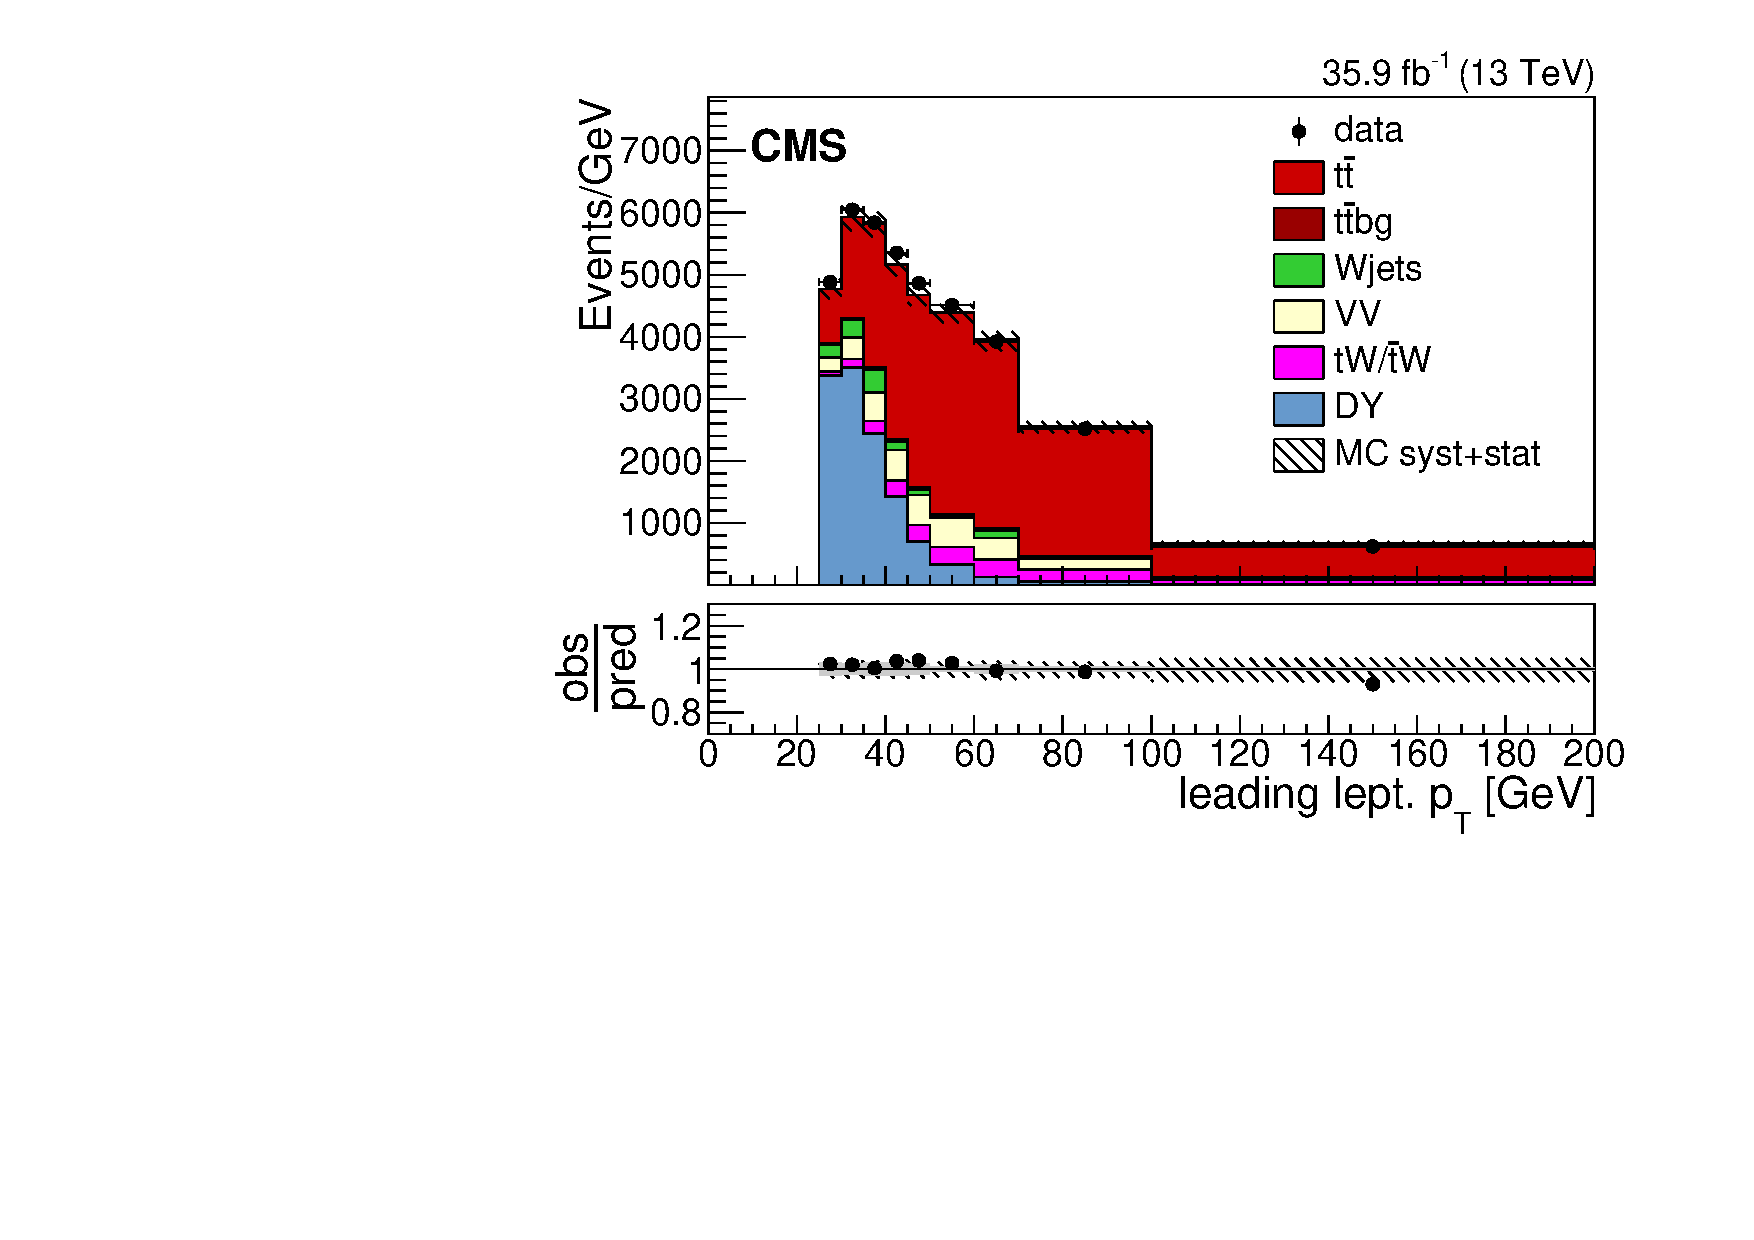
\includegraphics{CrossSection/Figures/ControlPlots/emu_sysnom/lead_lepton_pt_step_8.pdf}}
    \resizebox{0.48 \textwidth}{!}{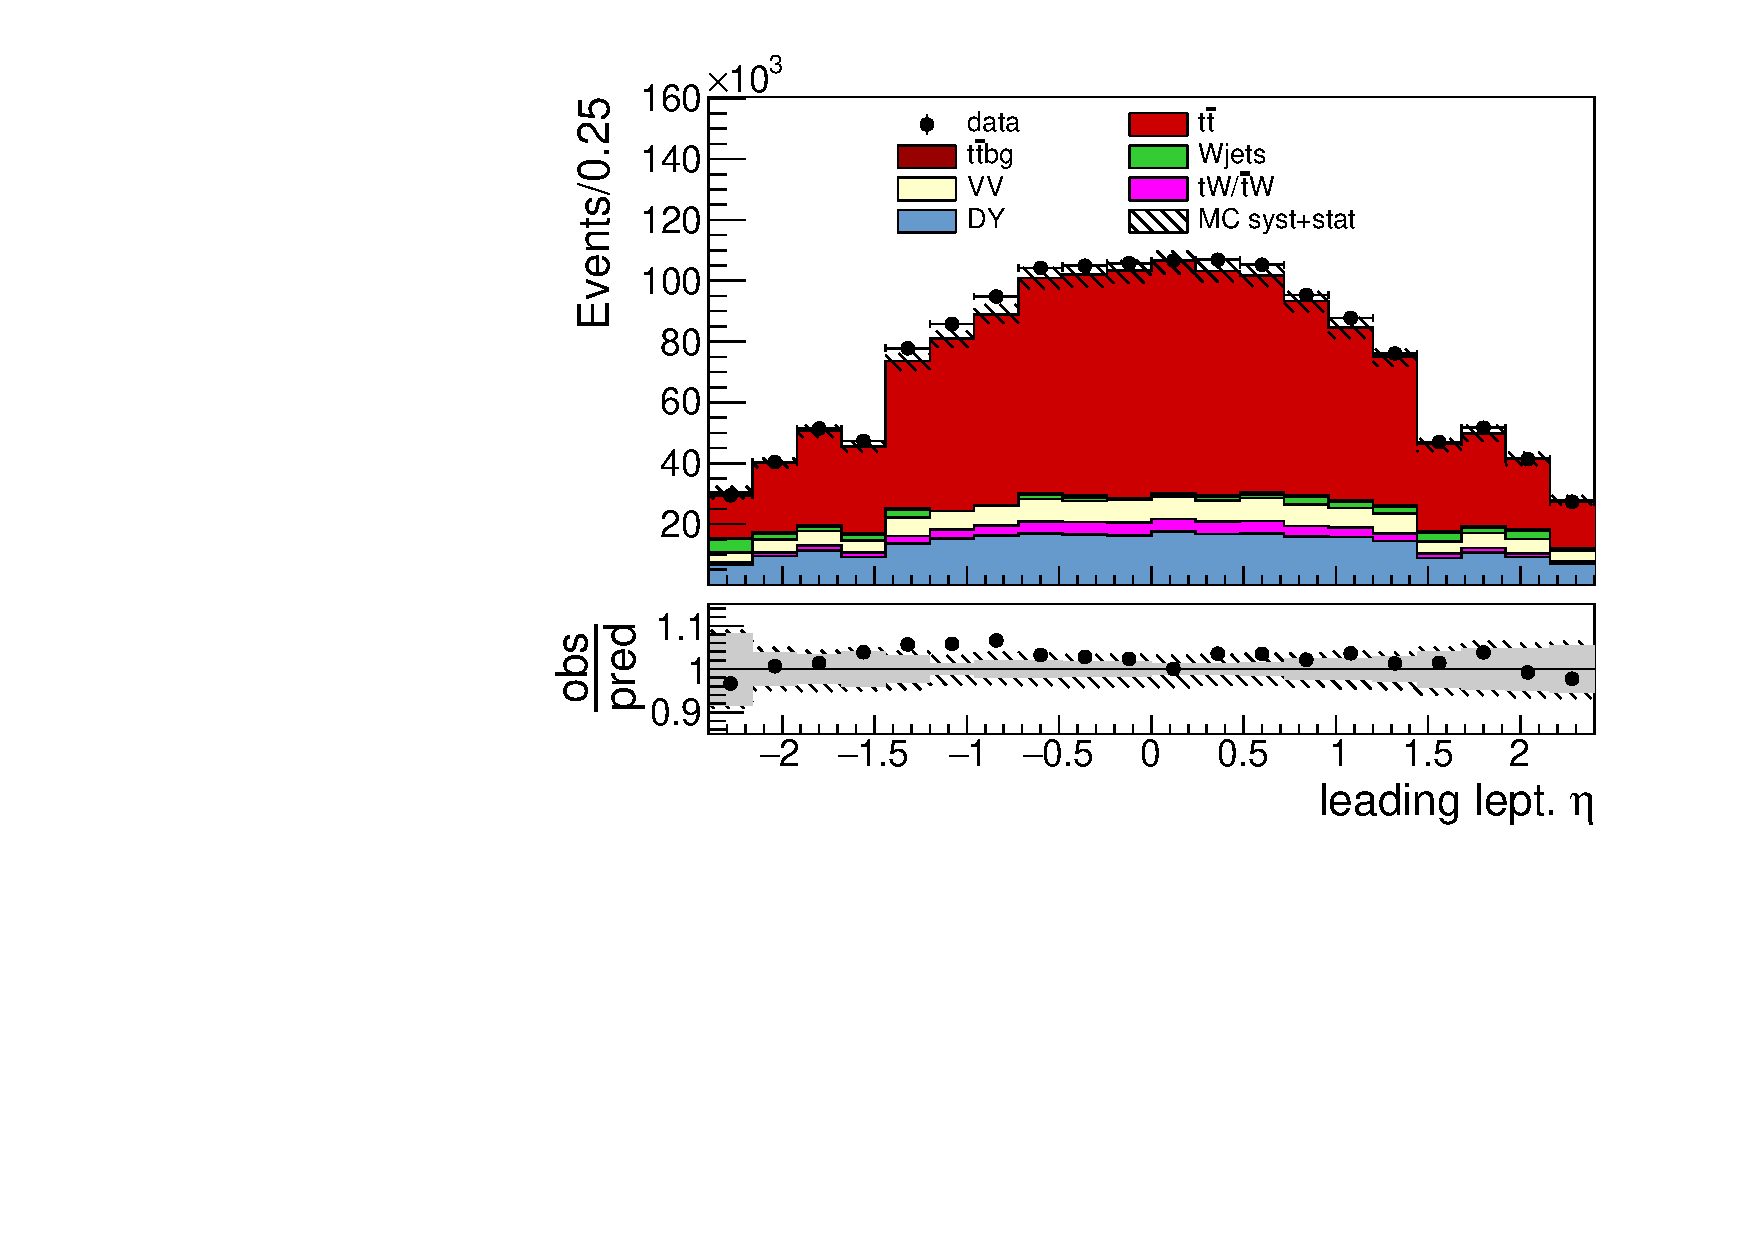
\includegraphics{CrossSection/Figures/ControlPlots/emu_sysnom/lead_lepton_eta_step_8.pdf}}
    \resizebox{0.48 \textwidth}{!}{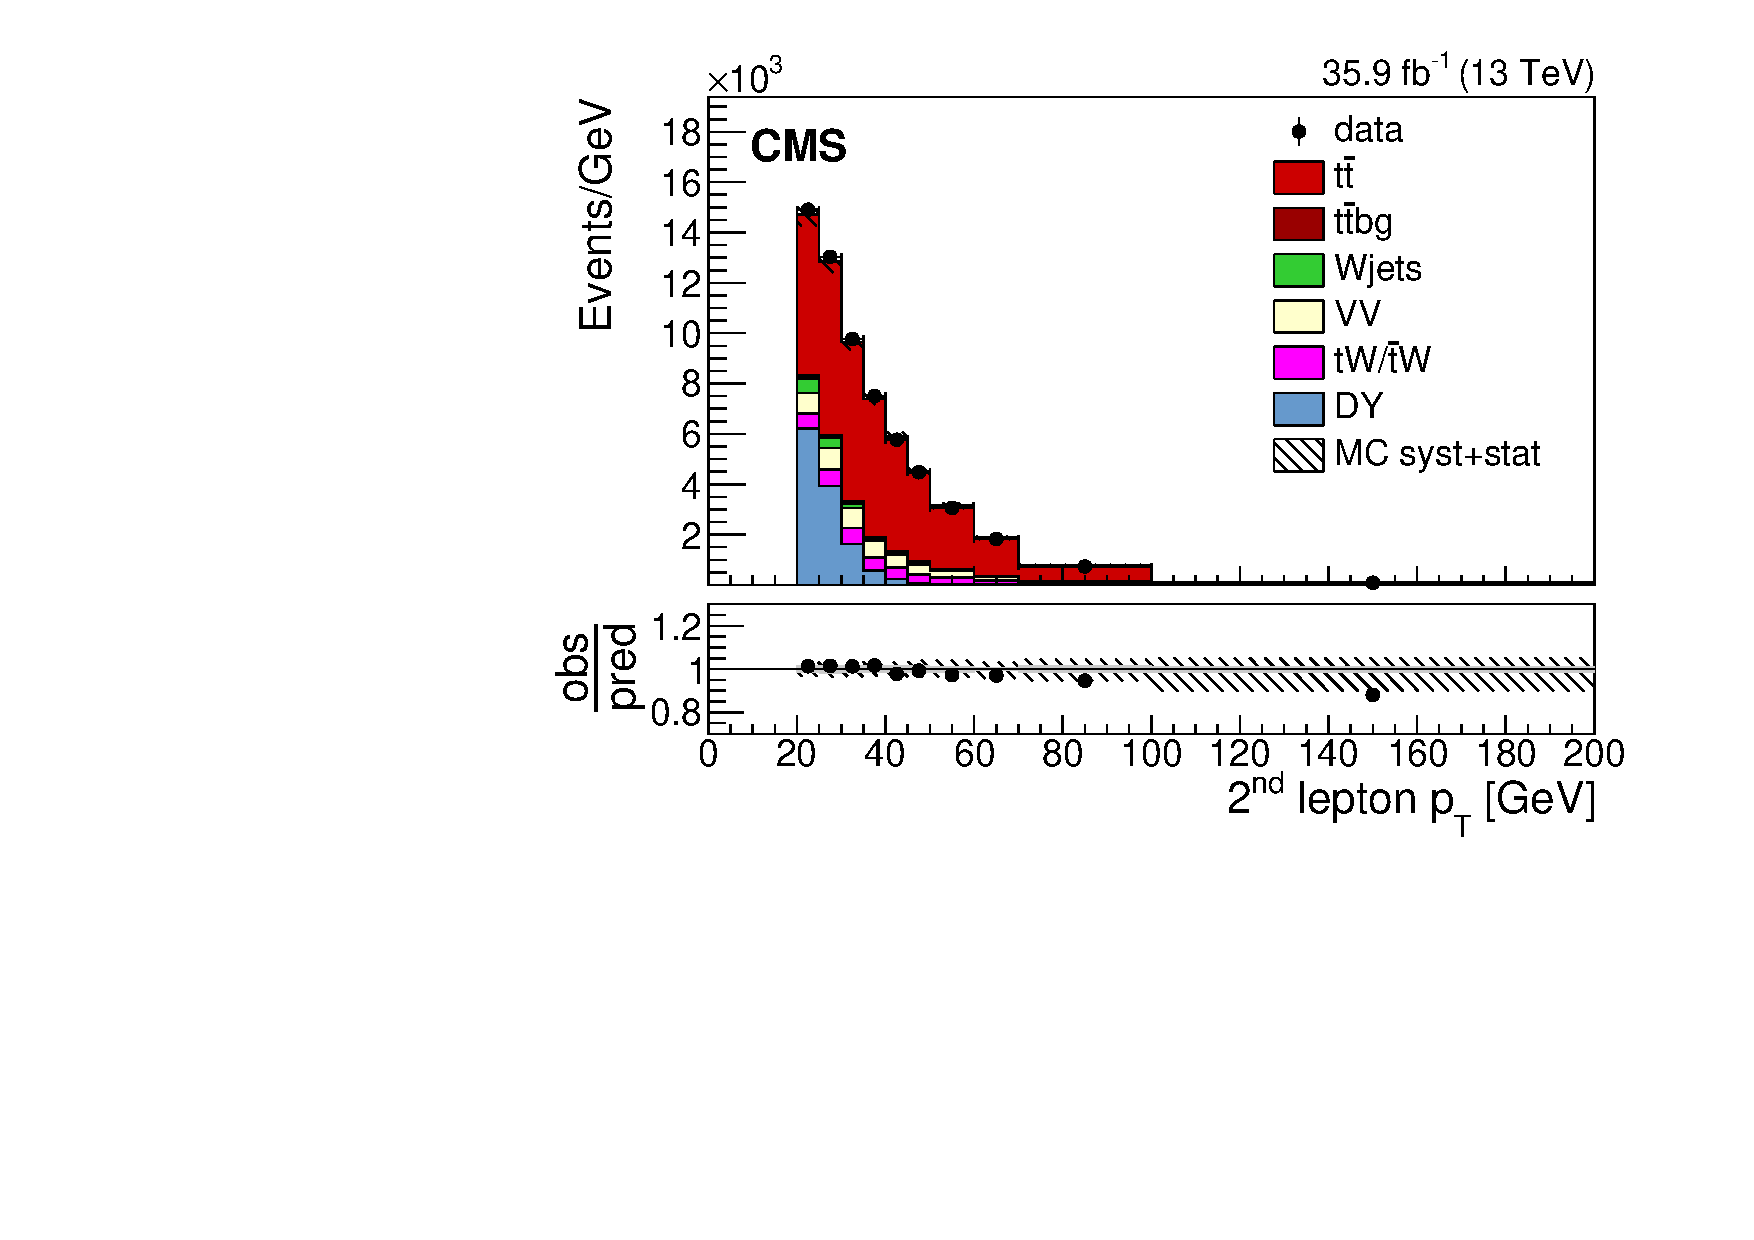
\includegraphics{CrossSection/Figures/ControlPlots/emu_sysnom/seclead_lepton_pt_step_8.pdf}}
    \resizebox{0.48 \textwidth}{!}{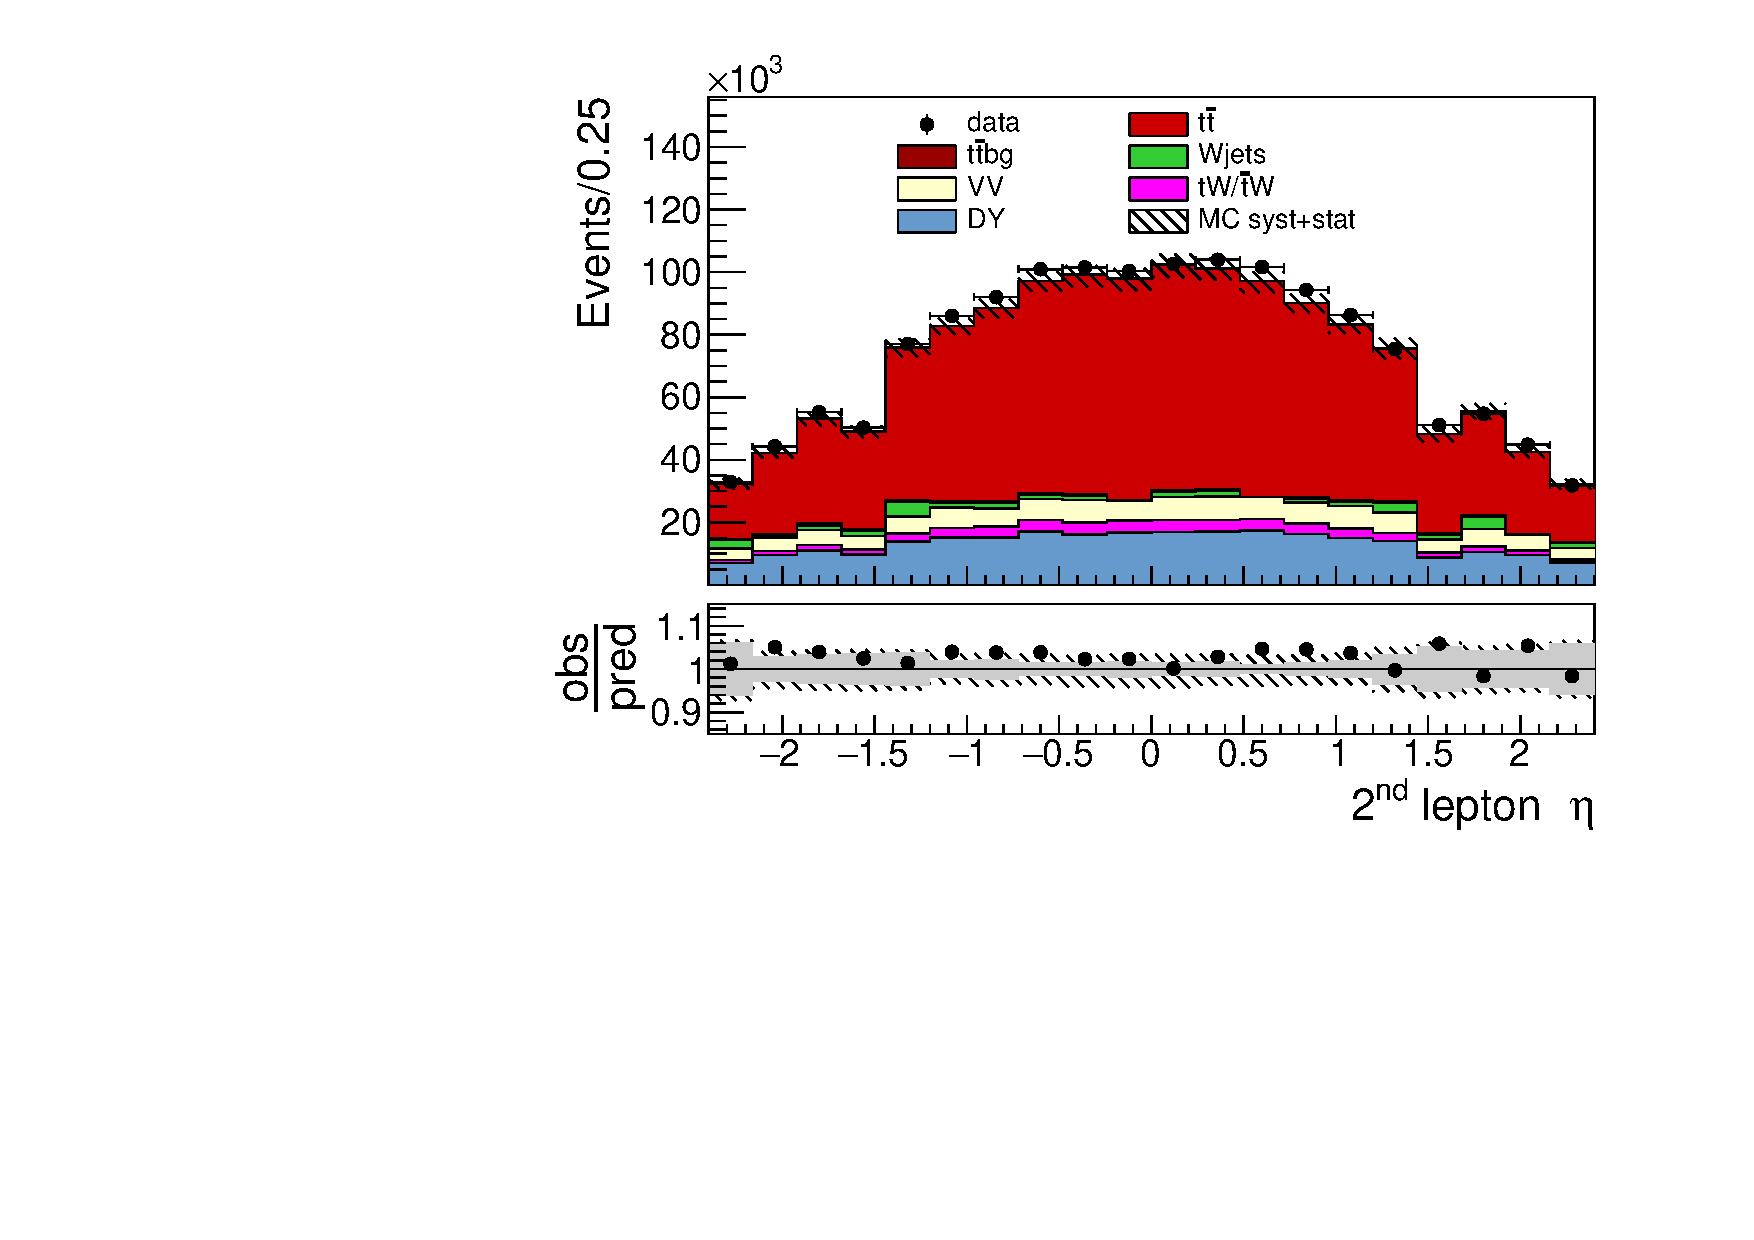
\includegraphics{CrossSection/Figures/ControlPlots/emu_sysnom/seclead_lepton_eta_step_8.pdf}}
    \resizebox{0.48 \textwidth}{!}{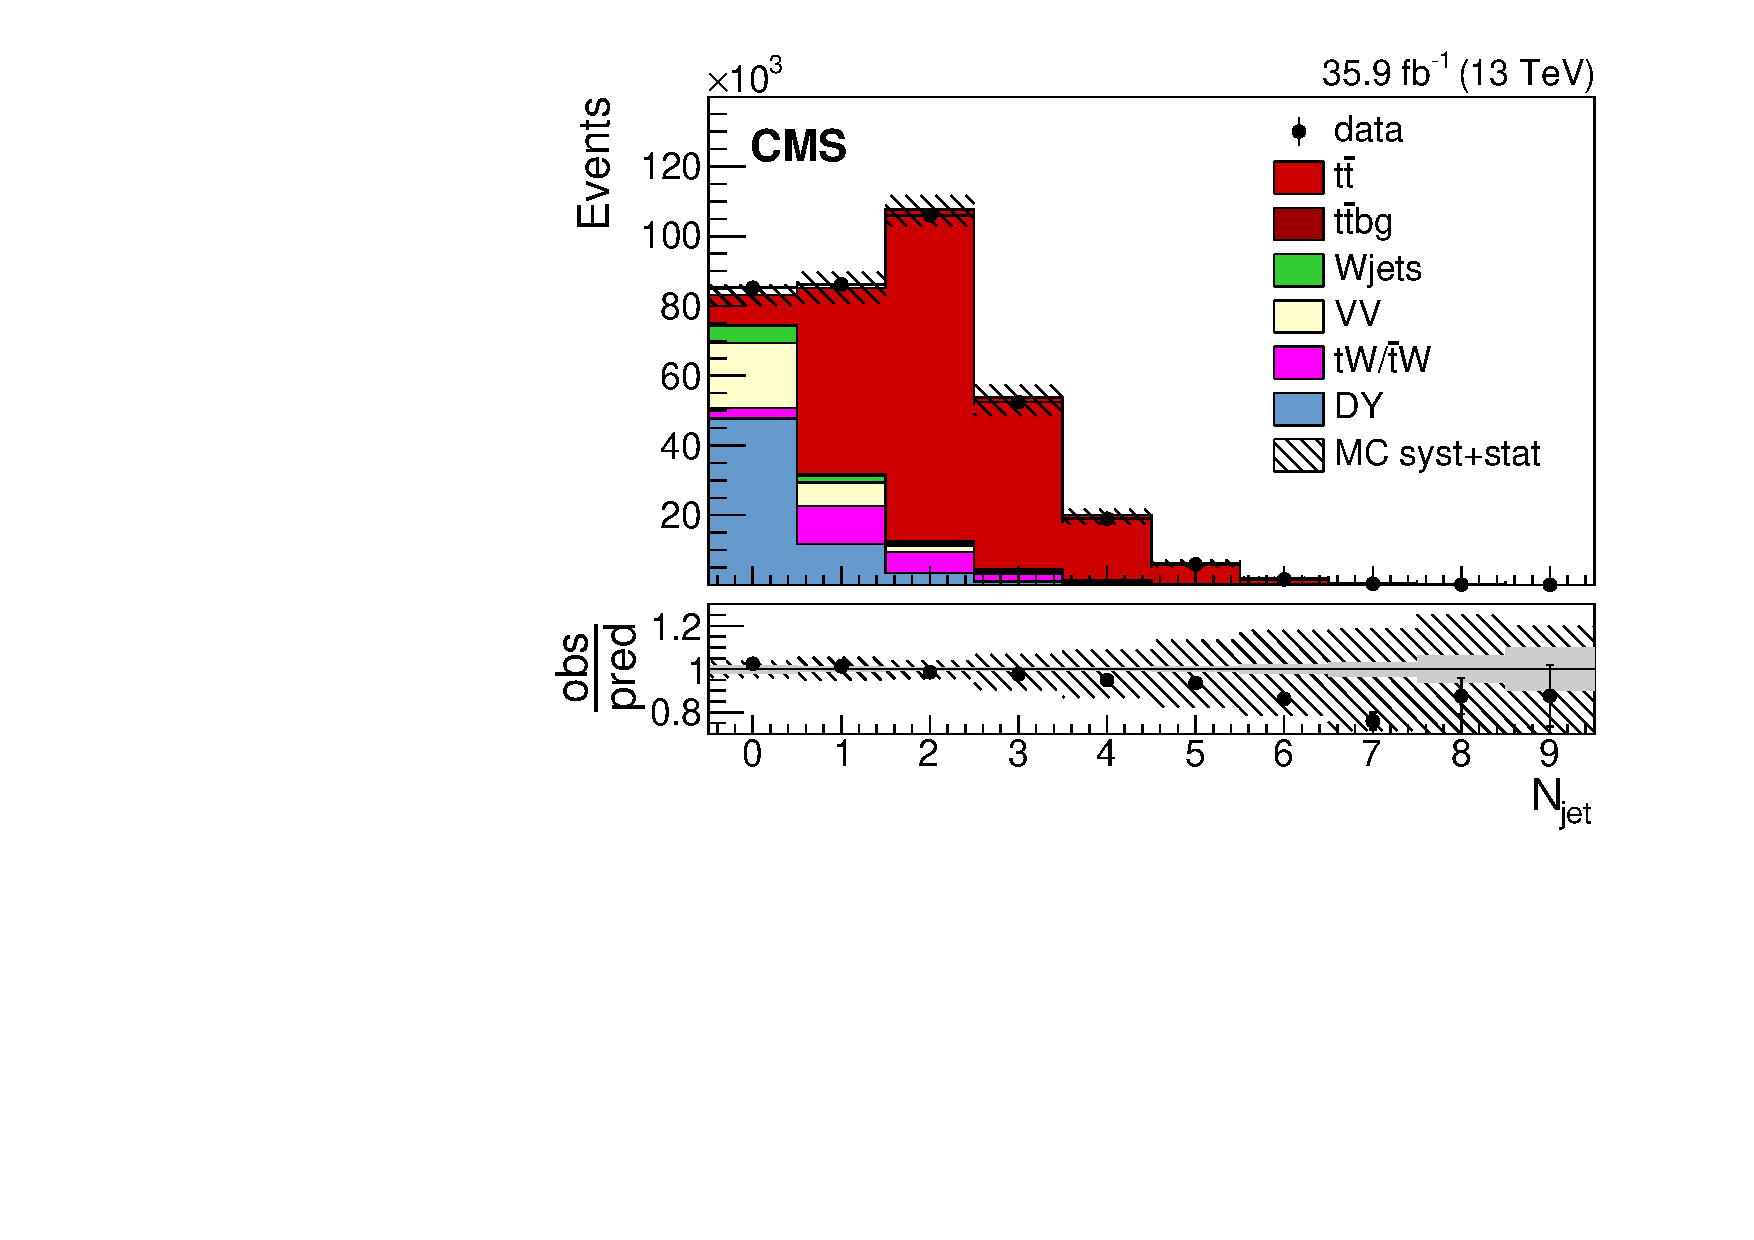
\includegraphics{CrossSection/Figures/ControlPlots/emu_sysnom/selected_jets_multi_step_8.pdf}}
    \resizebox{0.48 \textwidth}{!}{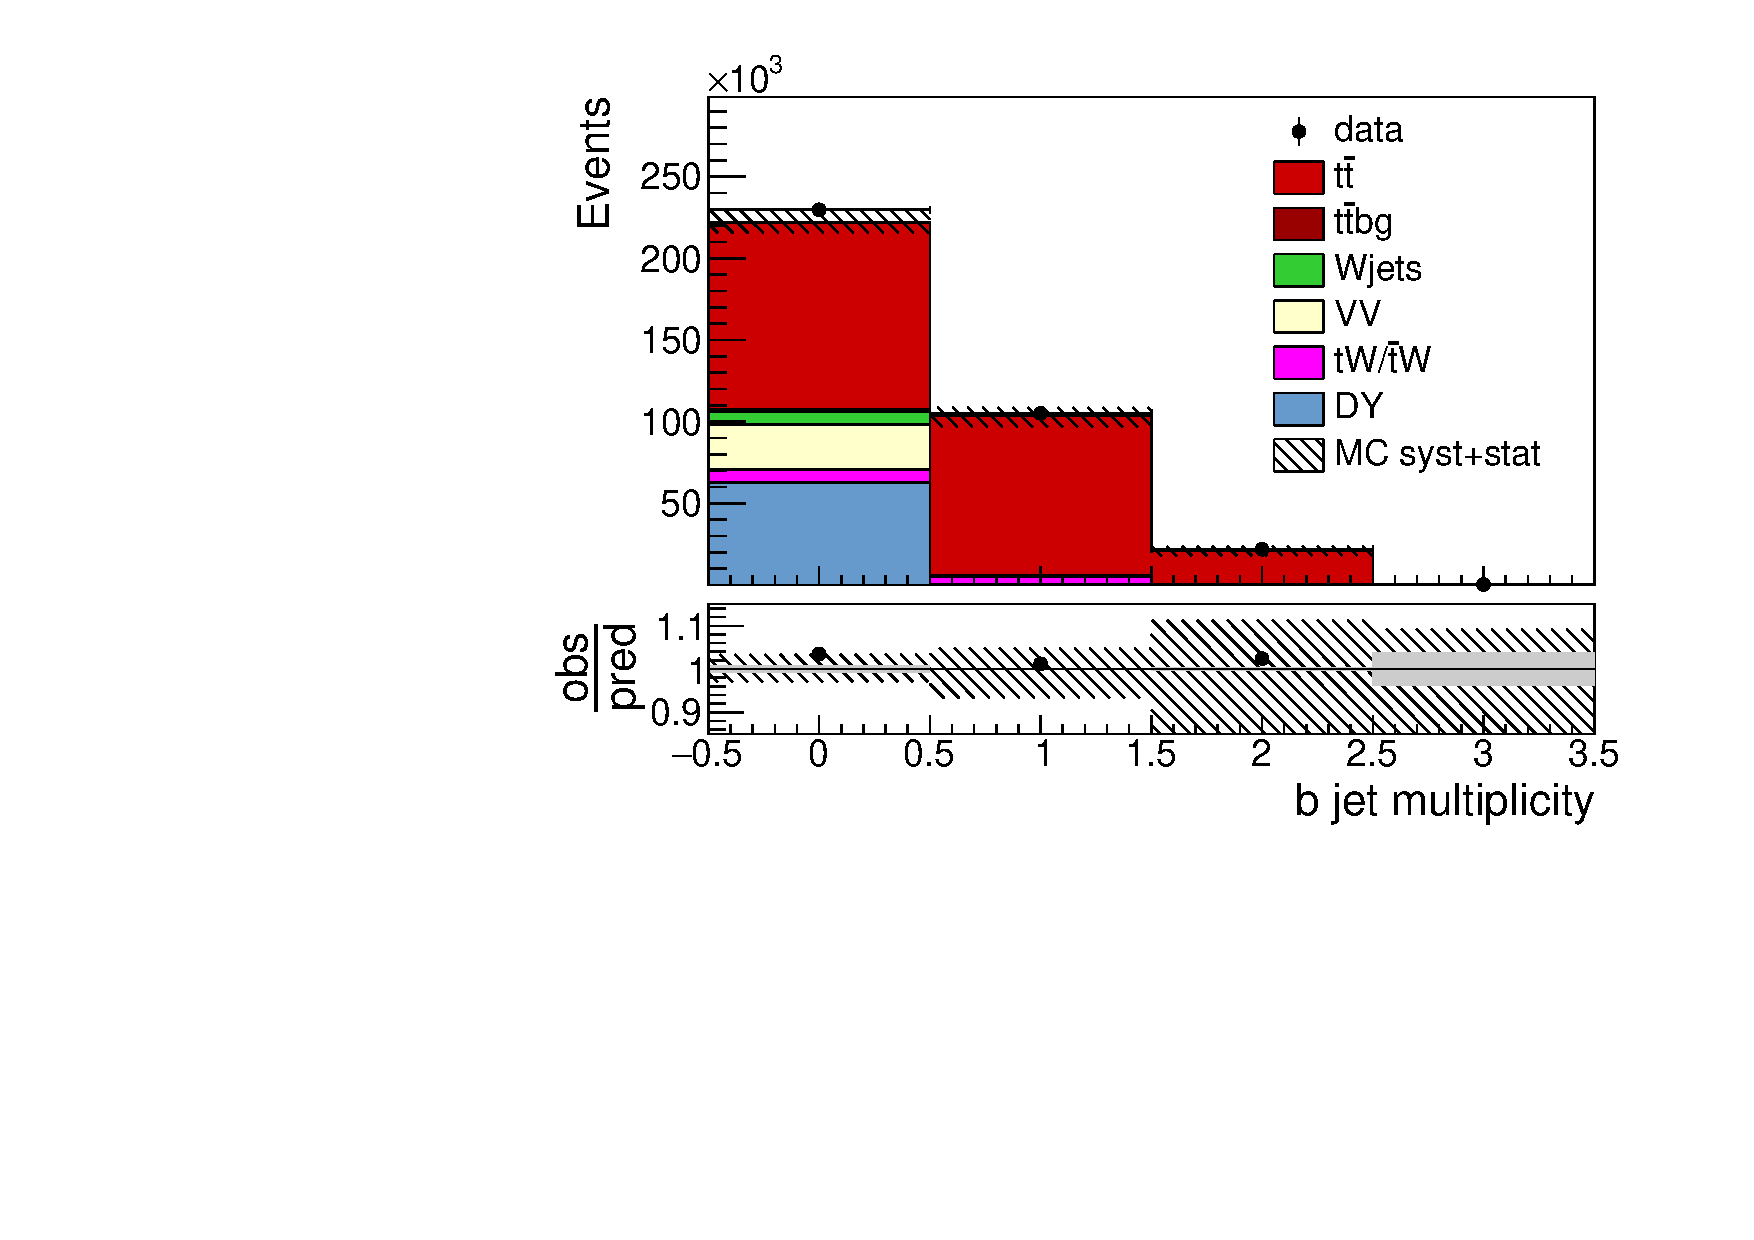
\includegraphics{CrossSection/Figures/ControlPlots/emu_sysnom/selected_b-jet_multi_step_8.pdf}}
      \caption{Transverse momentum (left) and pseudorapidity (right)
        of leading (first row) and second-leading (second row) lepton in the \emu channel after the
        event selection required by the \ttbar cross section
        extraction technique based on a simultaneous fit.
        Jet and b-jet multiplicity after the same selection steps are
        shown in the third row. The hatched
        bands correspond to the total uncertainty on the sum of the
        predicted yields. 
        %agrohsje , excluding luminosity and background
        %normalization uncertainties. 
        The ratios of data to the sum of the predicted yields are
        shown at the bottom of each plot. Here, the solid gray band
        represents the contribution of the statistical uncertainty.}  
       \label{fig:xsec_emu_ctrplots}
  \end{center}
\end{figure}

\begin{figure}[htbp!]
  \begin{center}
    \resizebox{0.48 \textwidth}{!}{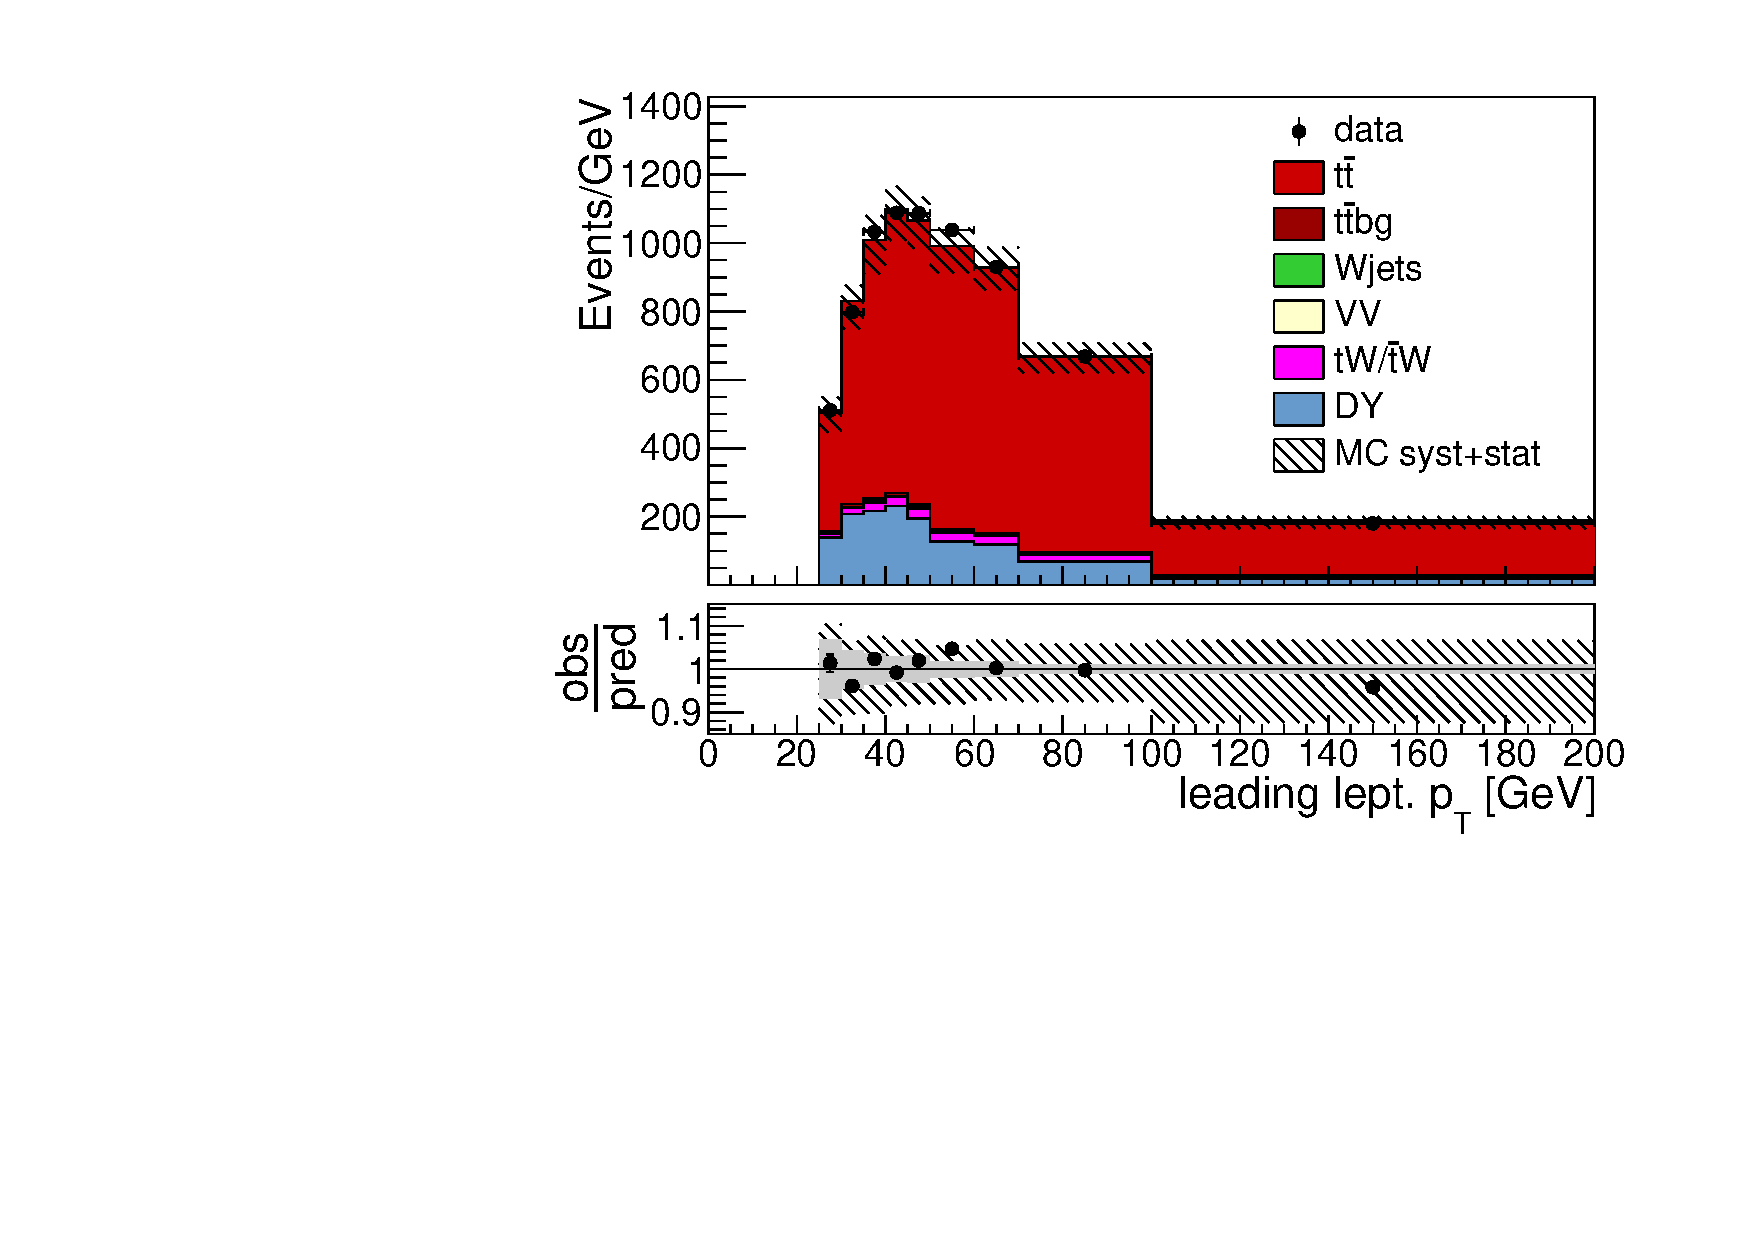
\includegraphics{CrossSection/Figures/ControlPlots/mumu_sysnom/lead_lepton_pt_step_8.pdf}}
    \resizebox{0.48 \textwidth}{!}{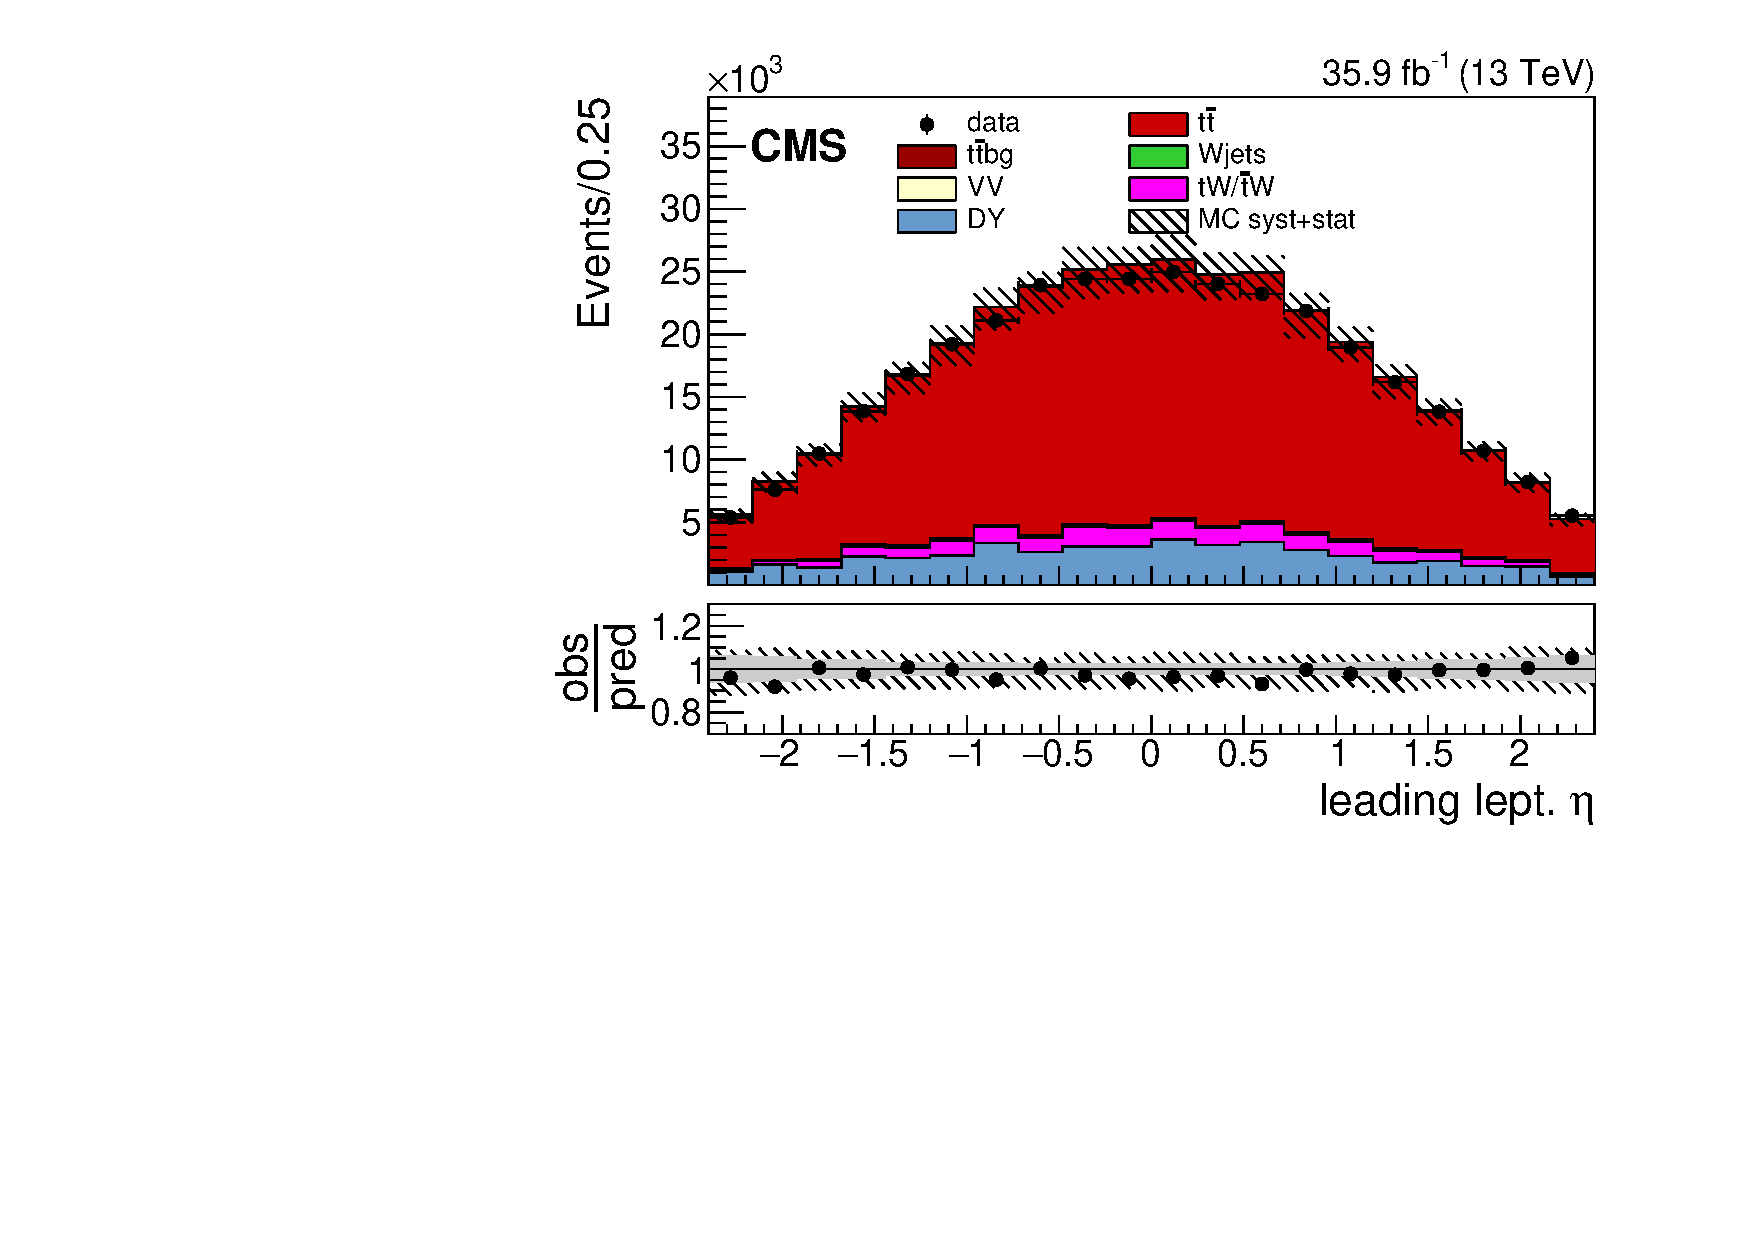
\includegraphics{CrossSection/Figures/ControlPlots/mumu_sysnom/lead_lepton_eta_step_8.pdf}}
    \resizebox{0.48 \textwidth}{!}{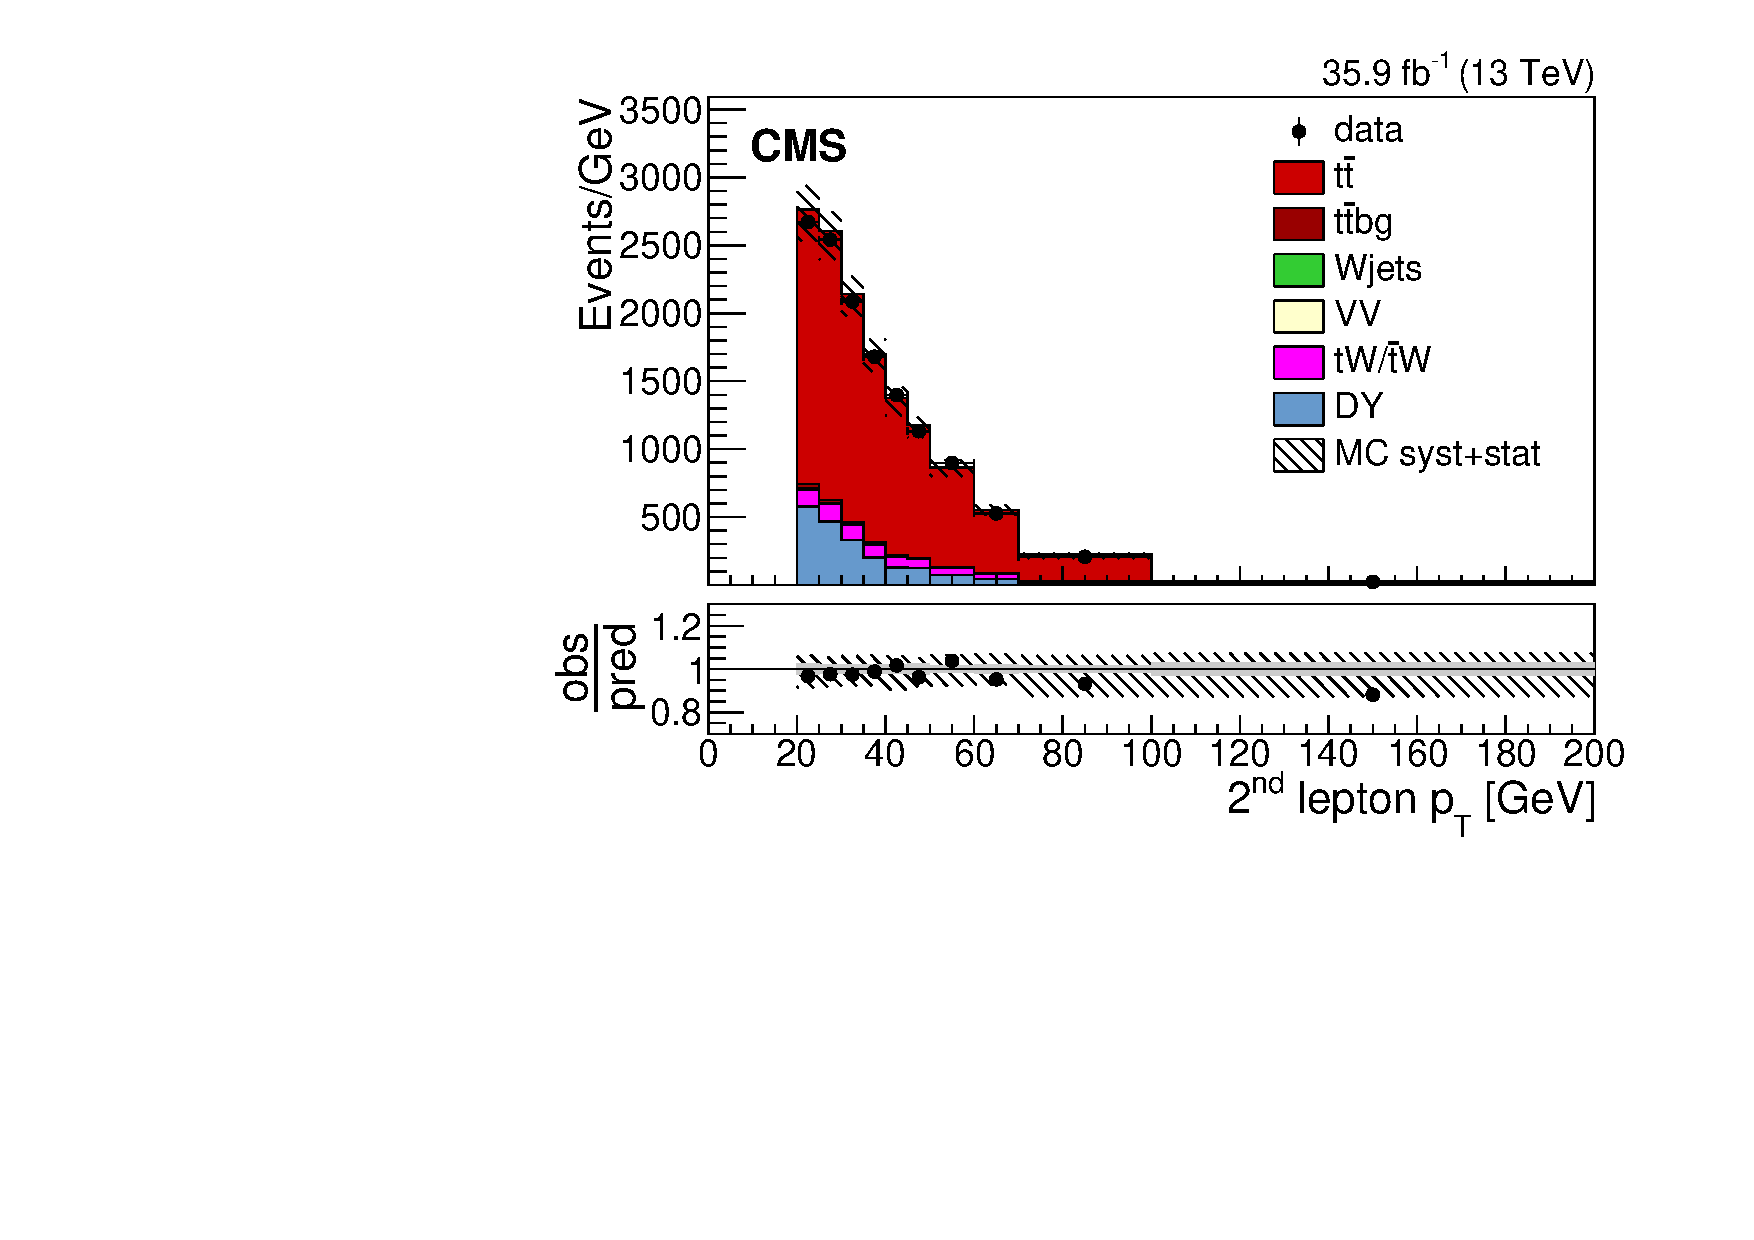
\includegraphics{CrossSection/Figures/ControlPlots/mumu_sysnom/seclead_lepton_pt_step_8.pdf}}
    \resizebox{0.48 \textwidth}{!}{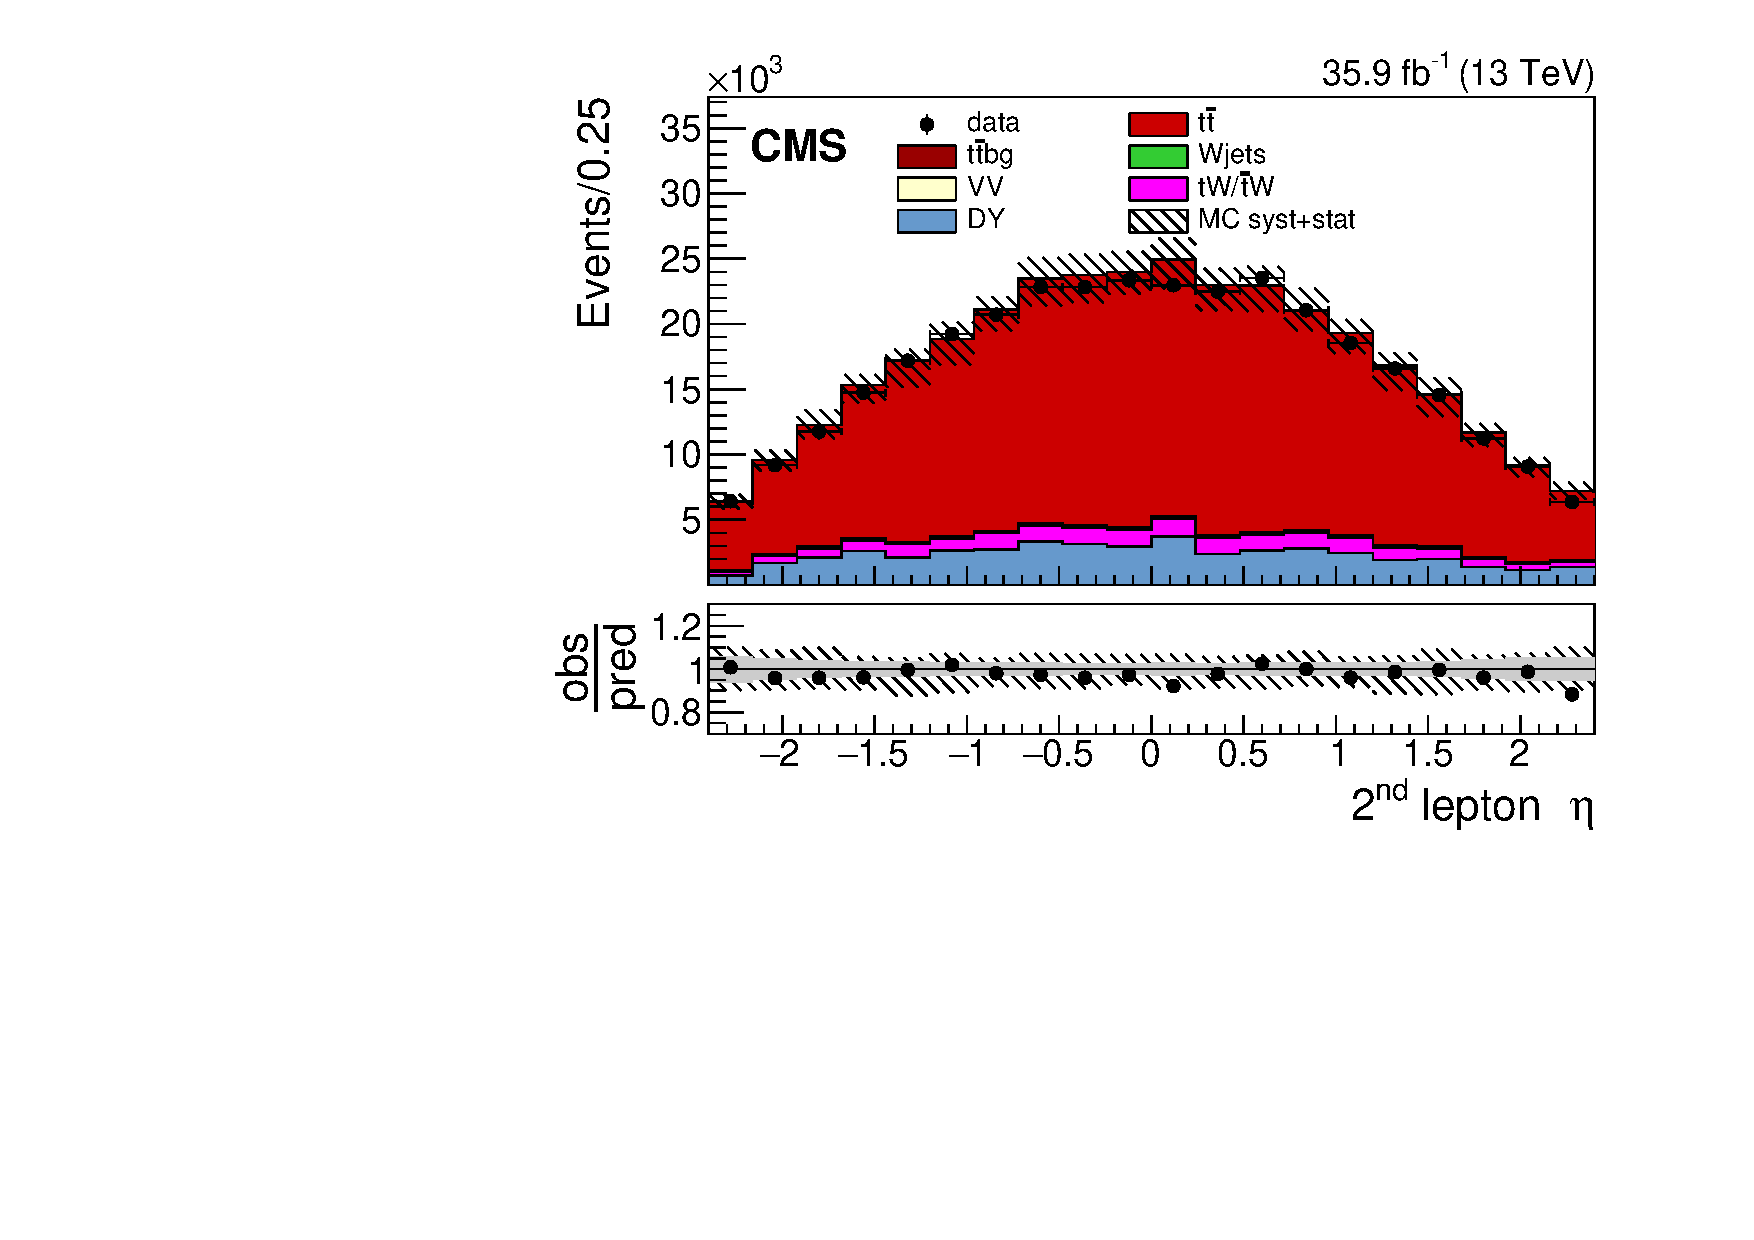
\includegraphics{CrossSection/Figures/ControlPlots/mumu_sysnom/seclead_lepton_eta_step_8.pdf}}
    \resizebox{0.48 \textwidth}{!}{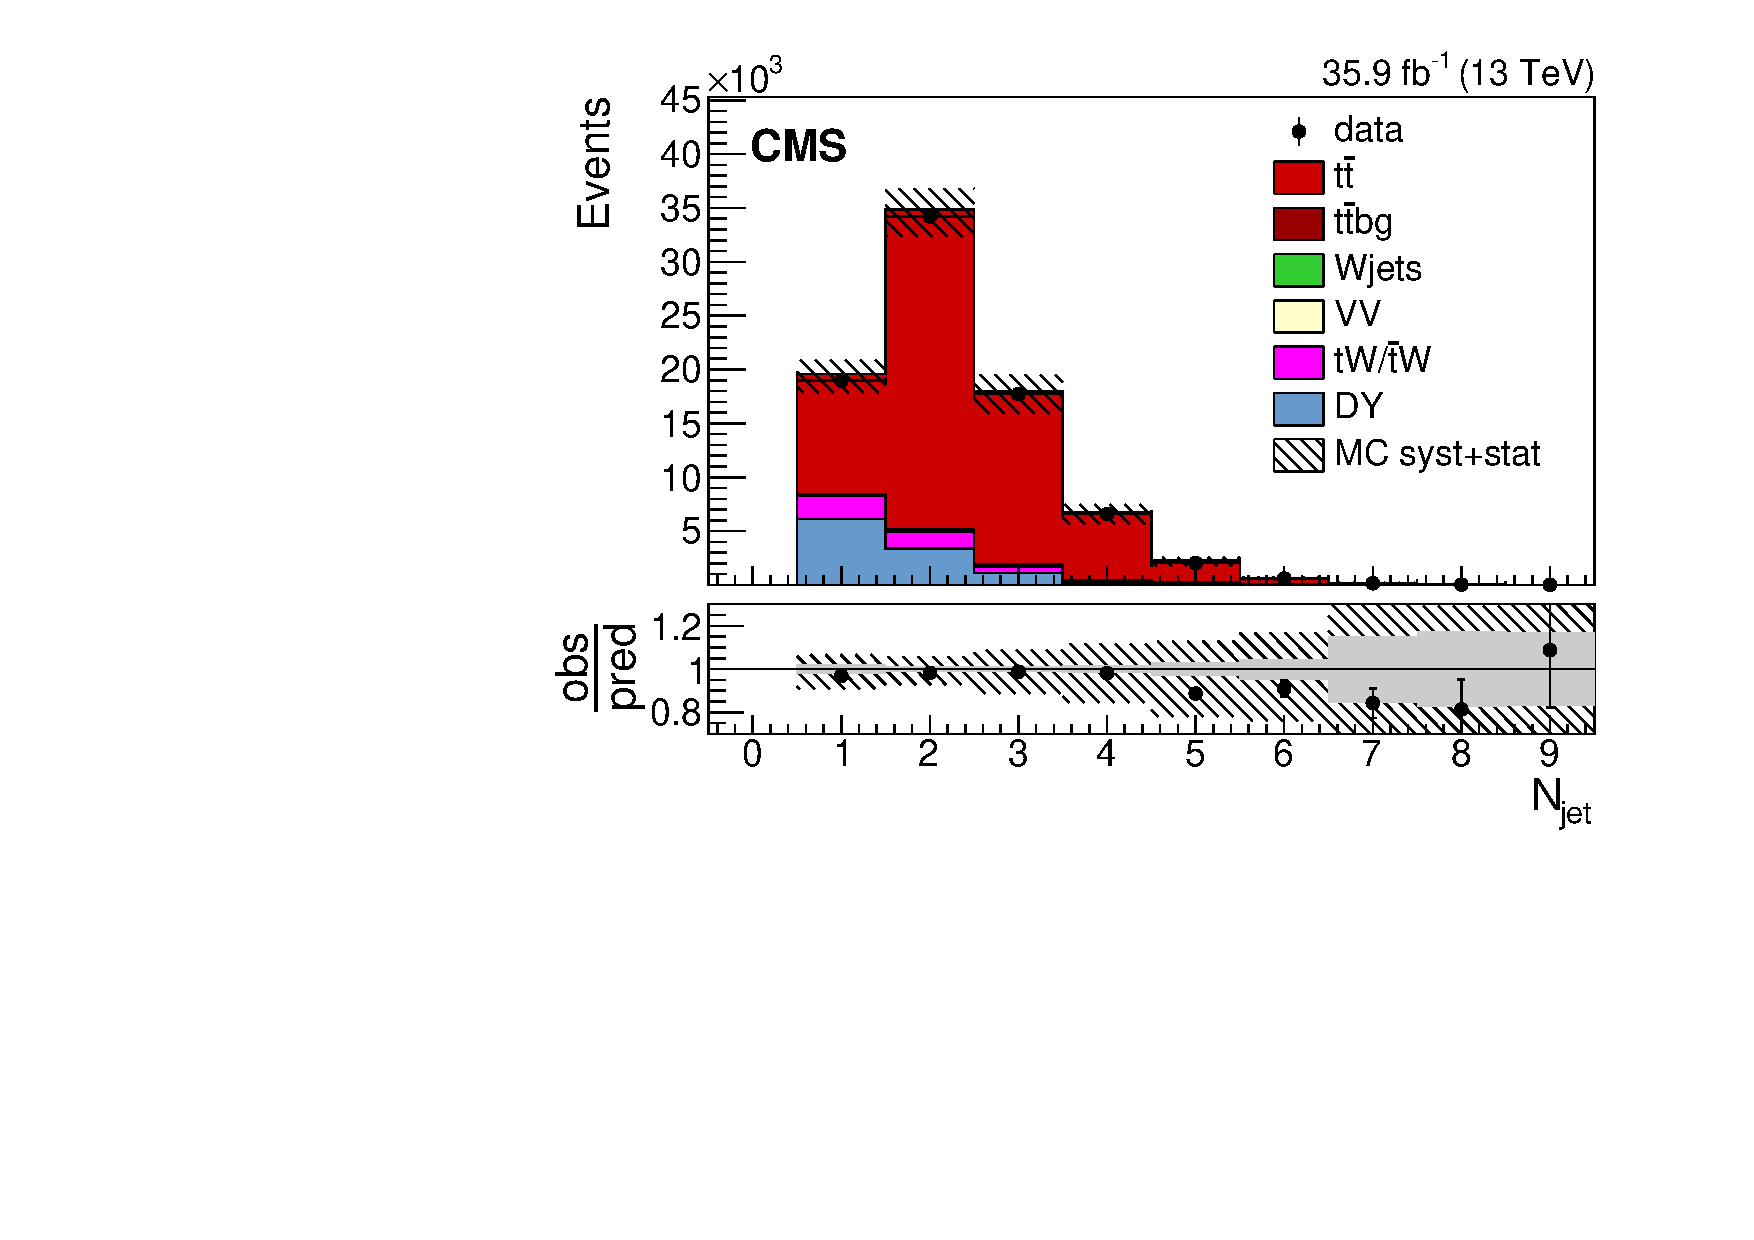
\includegraphics{CrossSection/Figures/ControlPlots/mumu_sysnom/selected_jets_multi_step_8.pdf}}
    \resizebox{0.48 \textwidth}{!}{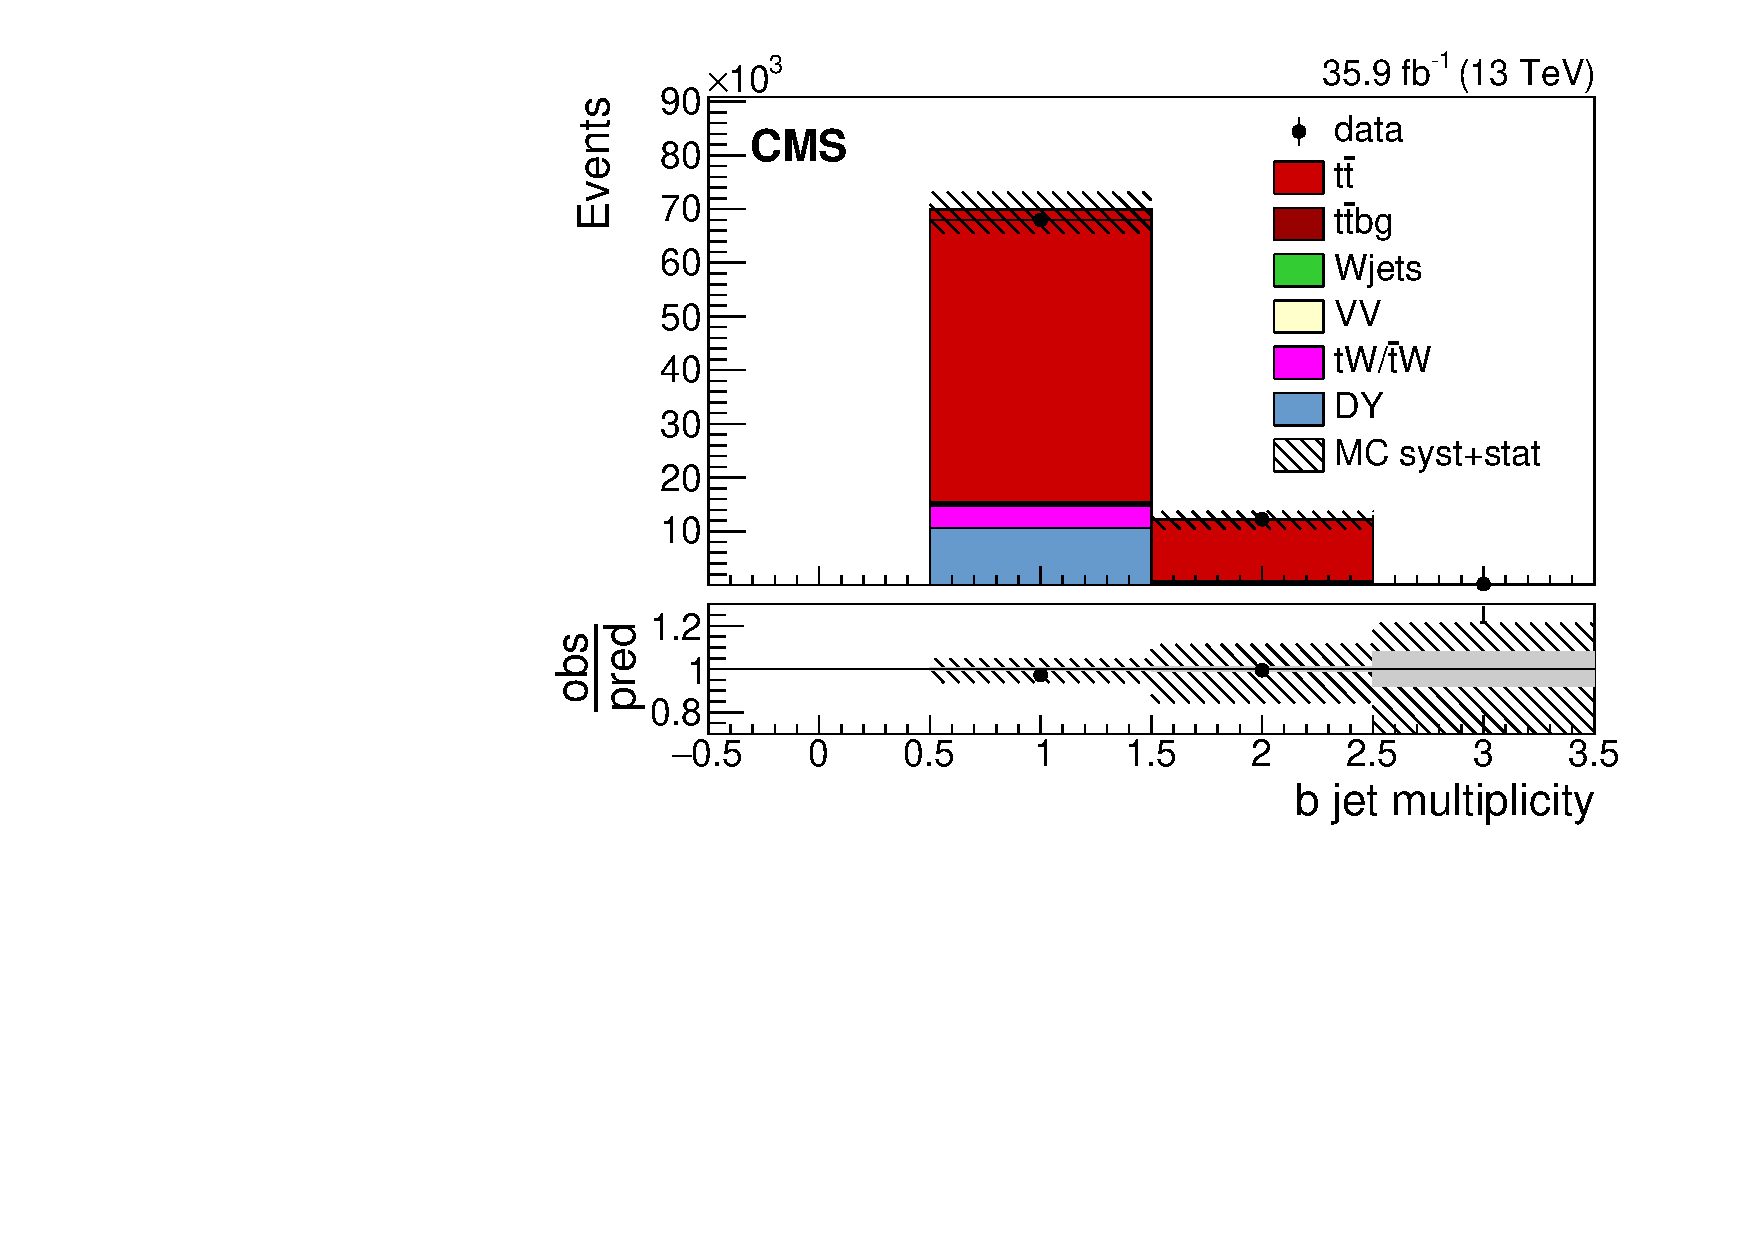
\includegraphics{CrossSection/Figures/ControlPlots/mumu_sysnom/selected_b-jet_multi_step_8.pdf}}
      \caption{Transverse momentum (left) and pseudorapidity (right)
        of leading (first row) and second-leading (second row) lepton in the \mumu channel after the
        event selection required by the \ttbar cross section
        extraction technique based on a simultaneous fit. Jet and b-jet multiplicity after the same selection steps are
        shown in the third row. The hatched
        bands correspond to the total uncertainty on the sum of the
        predicted yields. 
        %agrohsje , excluding luminosity and background
        %normalization uncertainties. 
        The ratios of data to the sum of the predicted yields are
        shown at the bottom of each plot. Here, the solid gray band
        represents the contribution of the statistical uncertainty.}  
       \label{fig:xsec_mumu_ctrplots}
  \end{center}
\end{figure}

\begin{figure}[htbp!]
  \begin{center}
    \resizebox{0.48 \textwidth}{!}{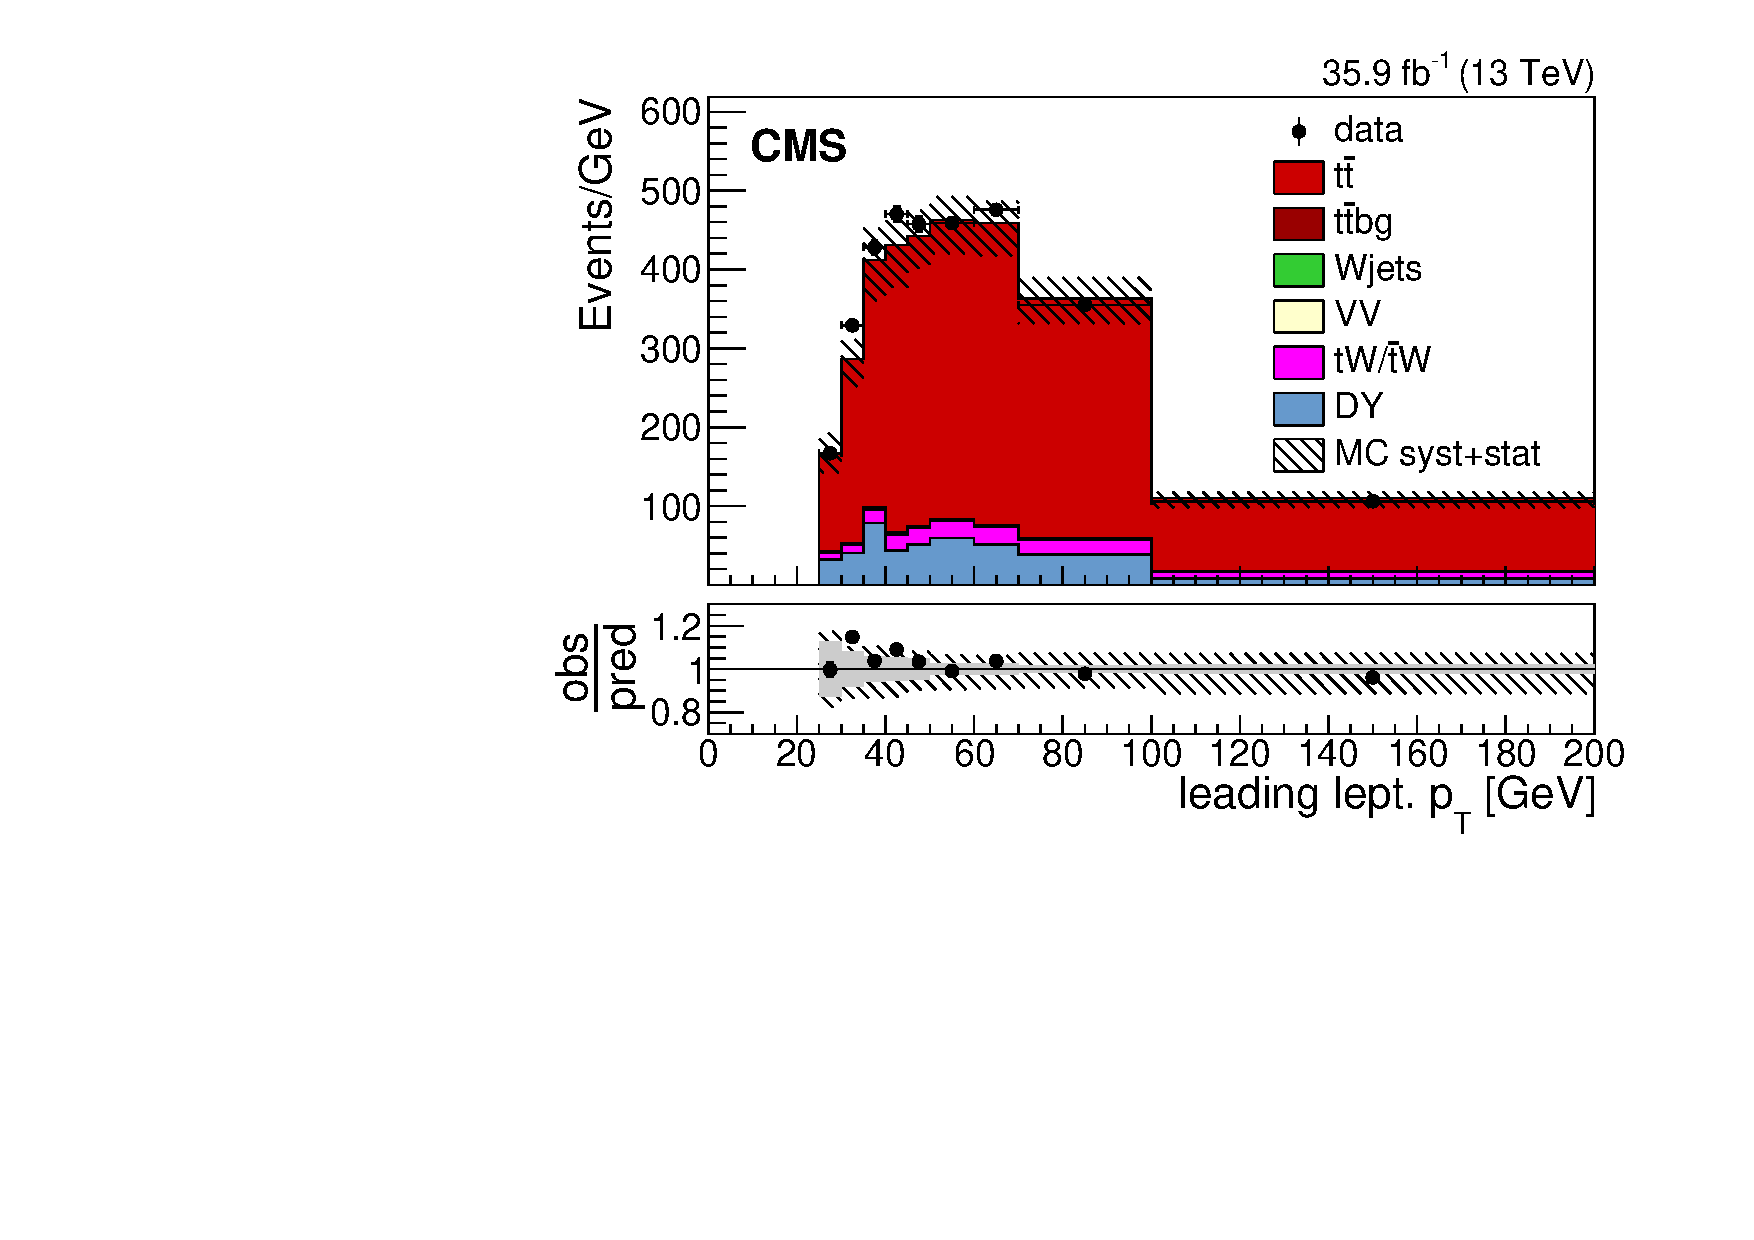
\includegraphics{CrossSection/Figures/ControlPlots/ee_sysnom/lead_lepton_pt_step_8.pdf}}
    \resizebox{0.48 \textwidth}{!}{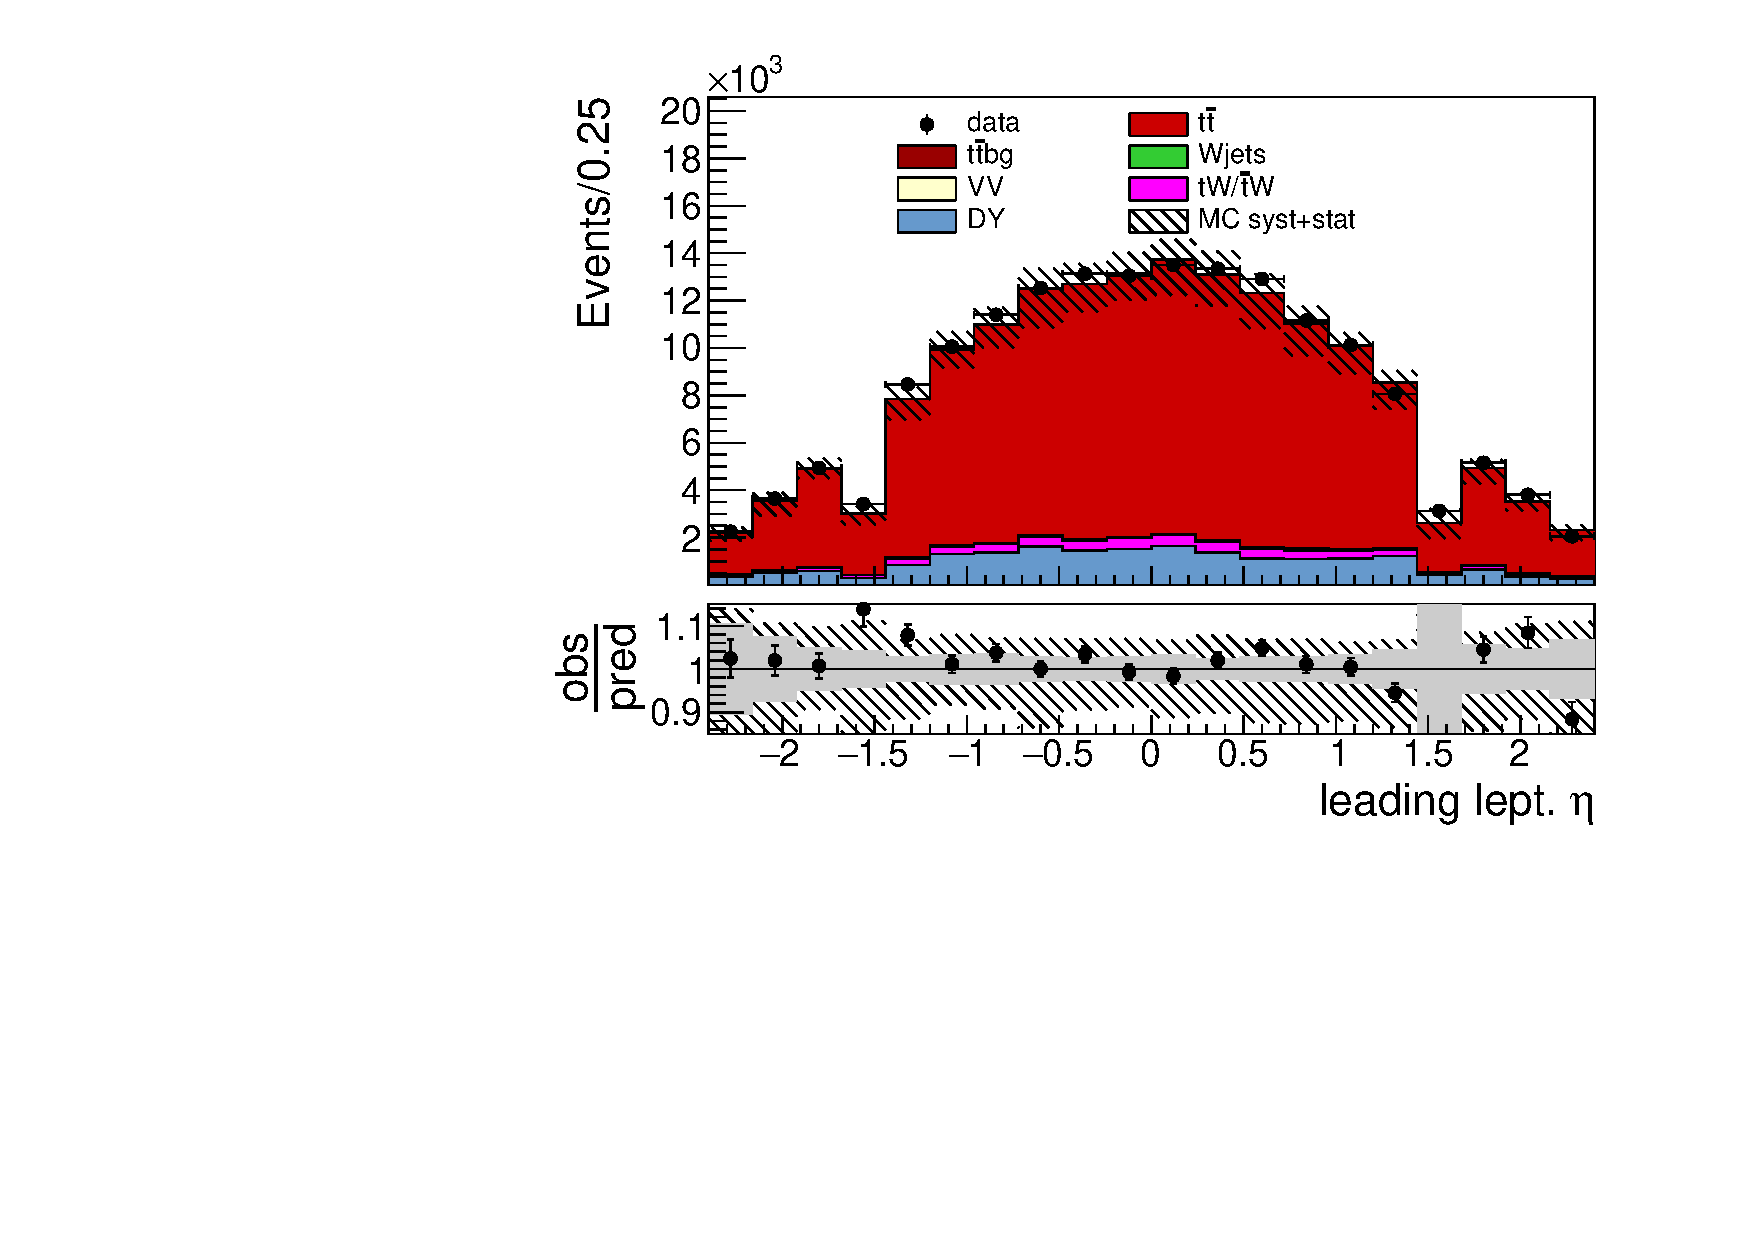
\includegraphics{CrossSection/Figures/ControlPlots/ee_sysnom/lead_lepton_eta_step_8.pdf}}
    \resizebox{0.48 \textwidth}{!}{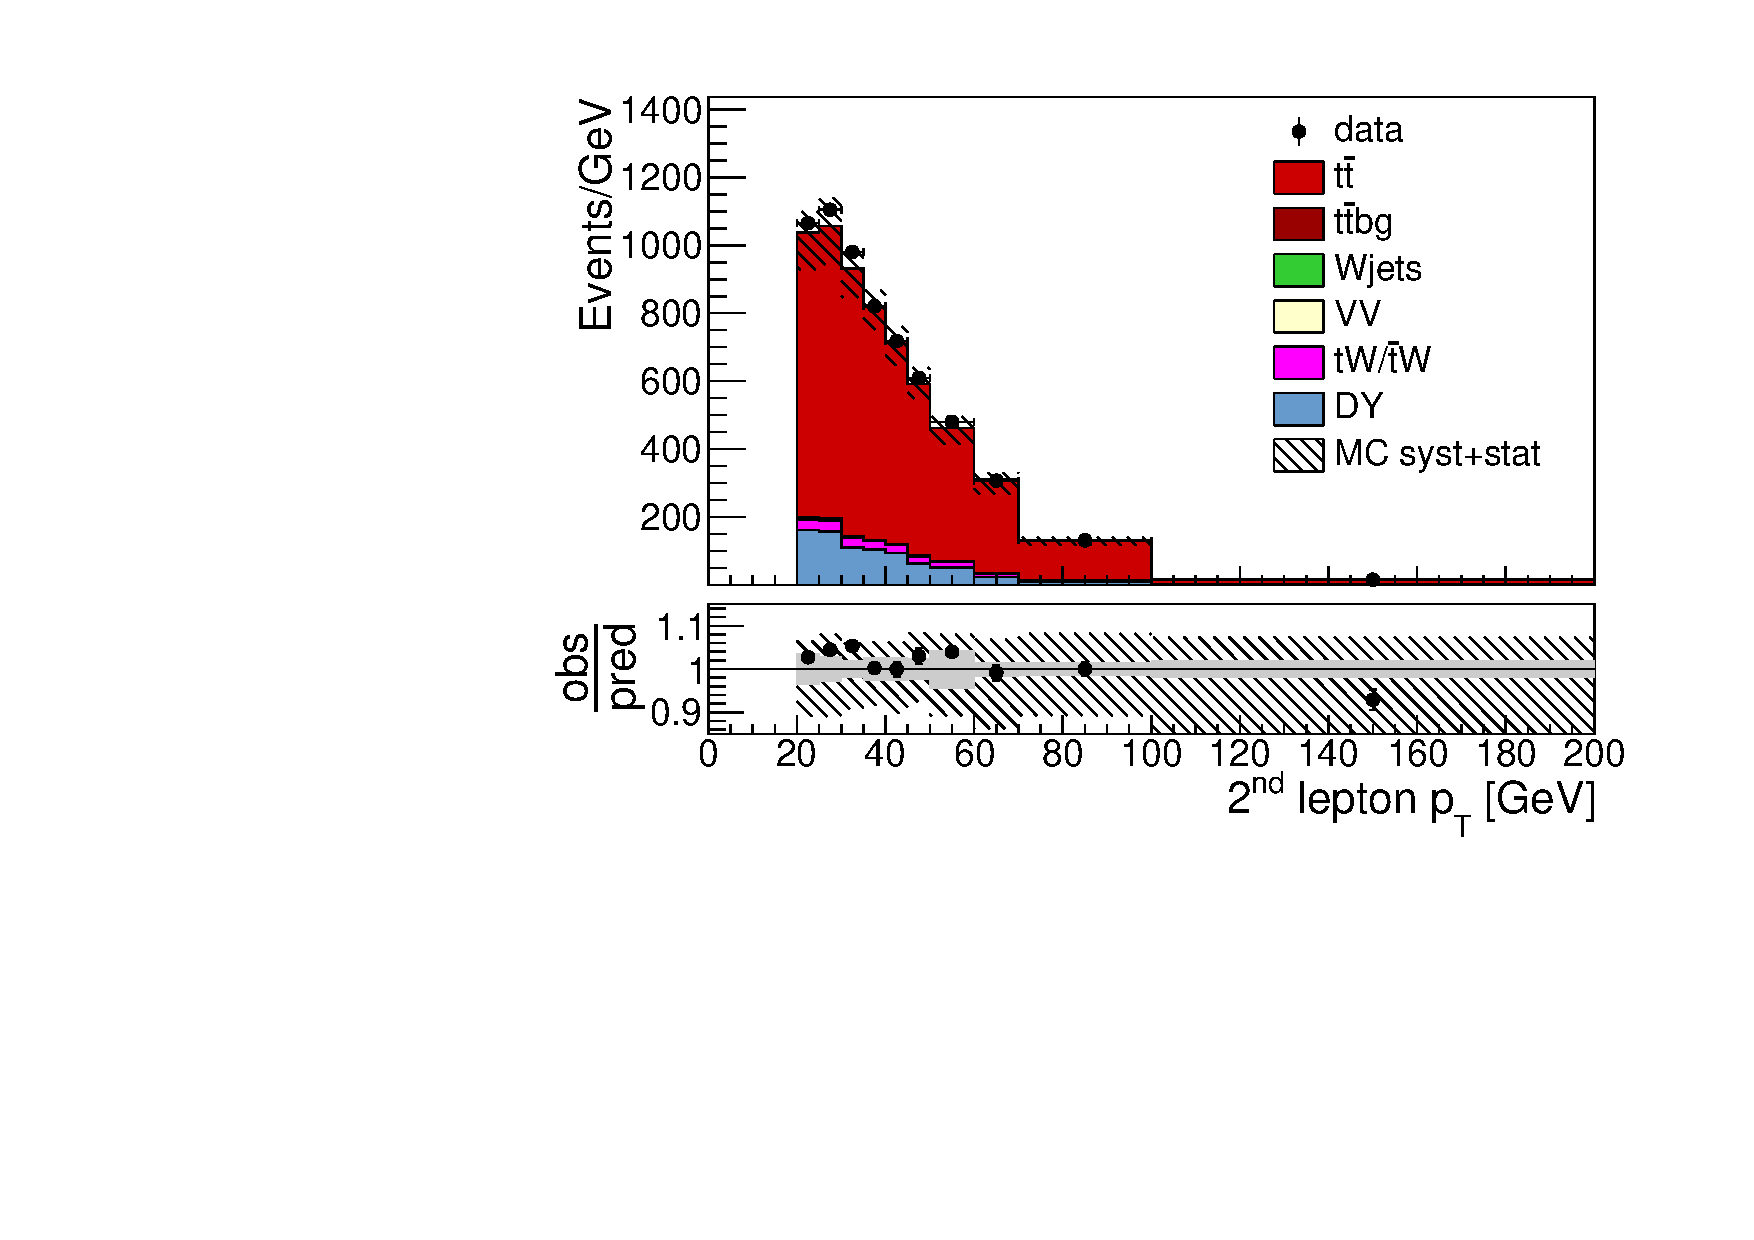
\includegraphics{CrossSection/Figures/ControlPlots/ee_sysnom/seclead_lepton_pt_step_8.pdf}}
    \resizebox{0.48 \textwidth}{!}{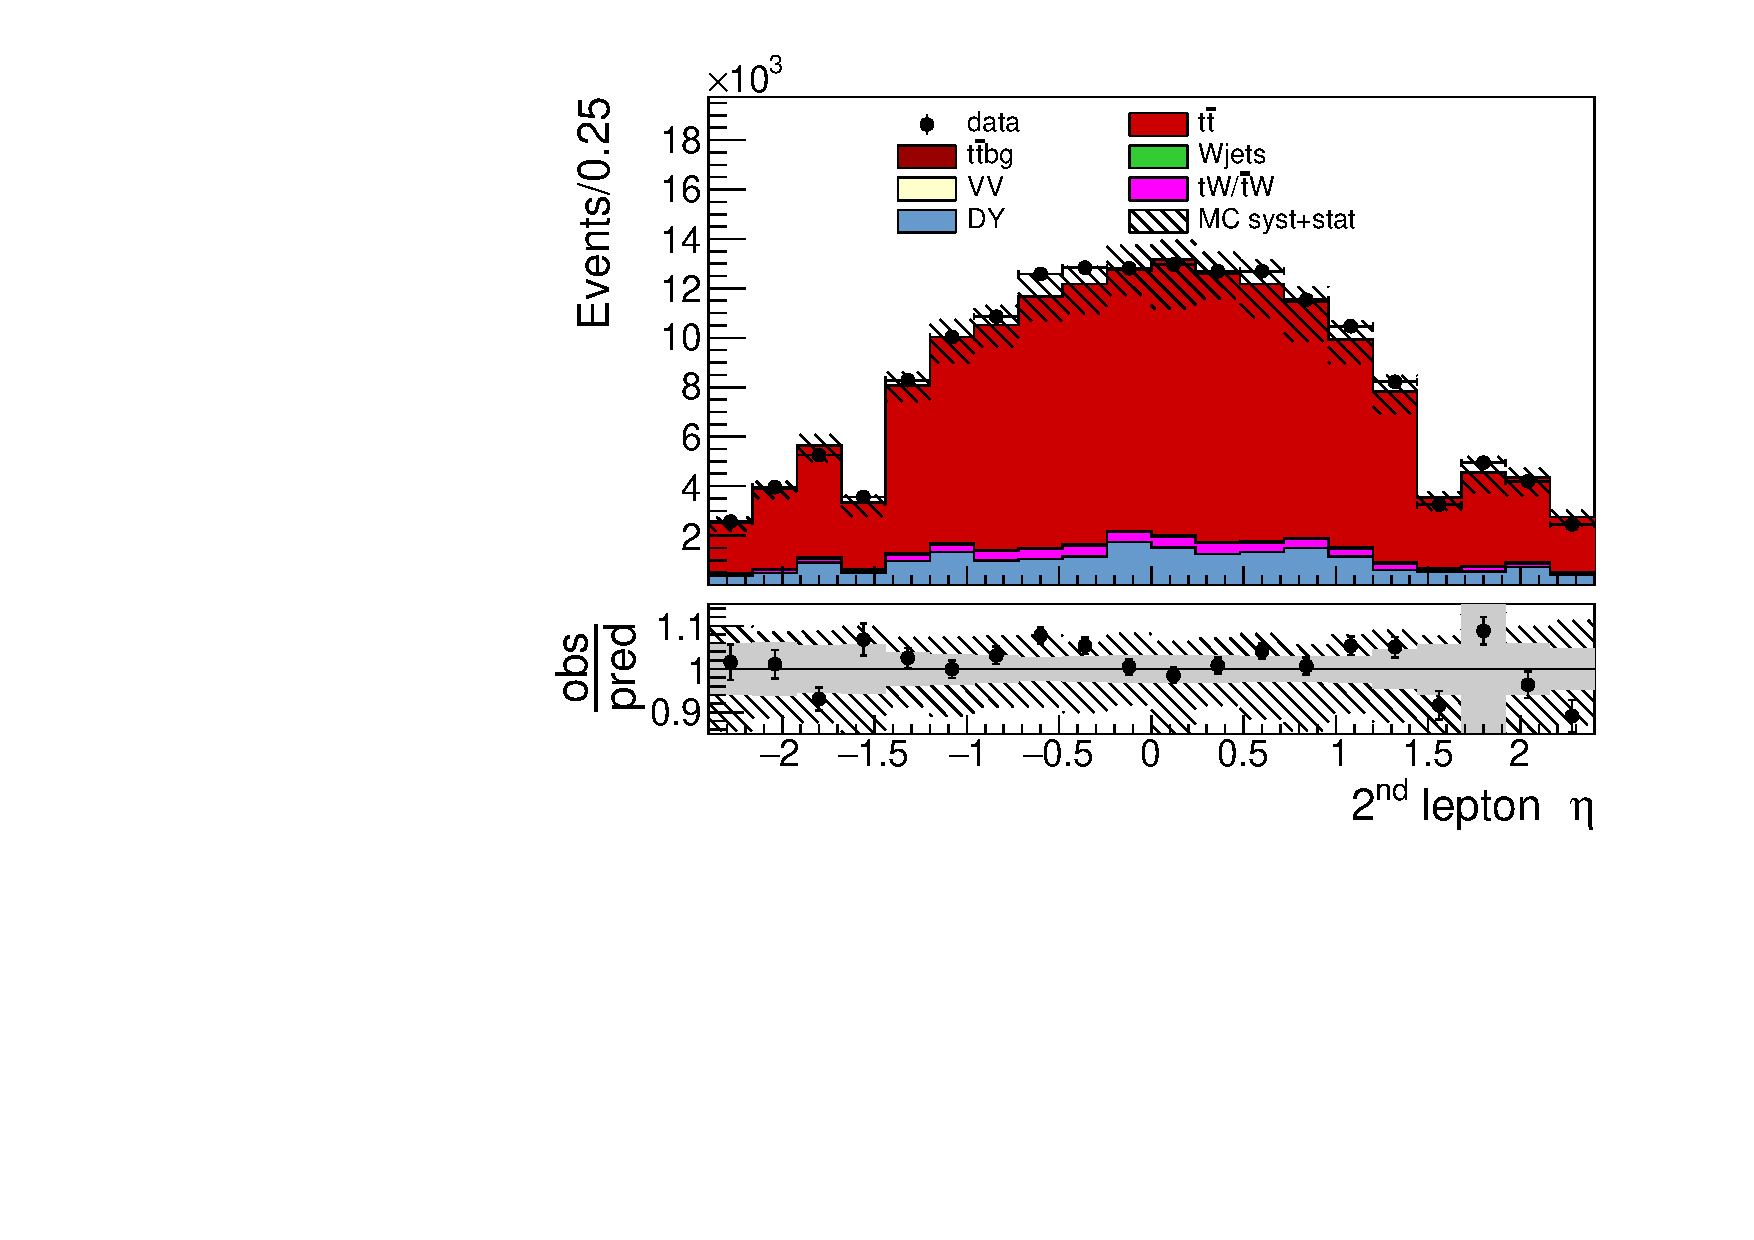
\includegraphics{CrossSection/Figures/ControlPlots/ee_sysnom/seclead_lepton_eta_step_8.pdf}}
    \resizebox{0.48 \textwidth}{!}{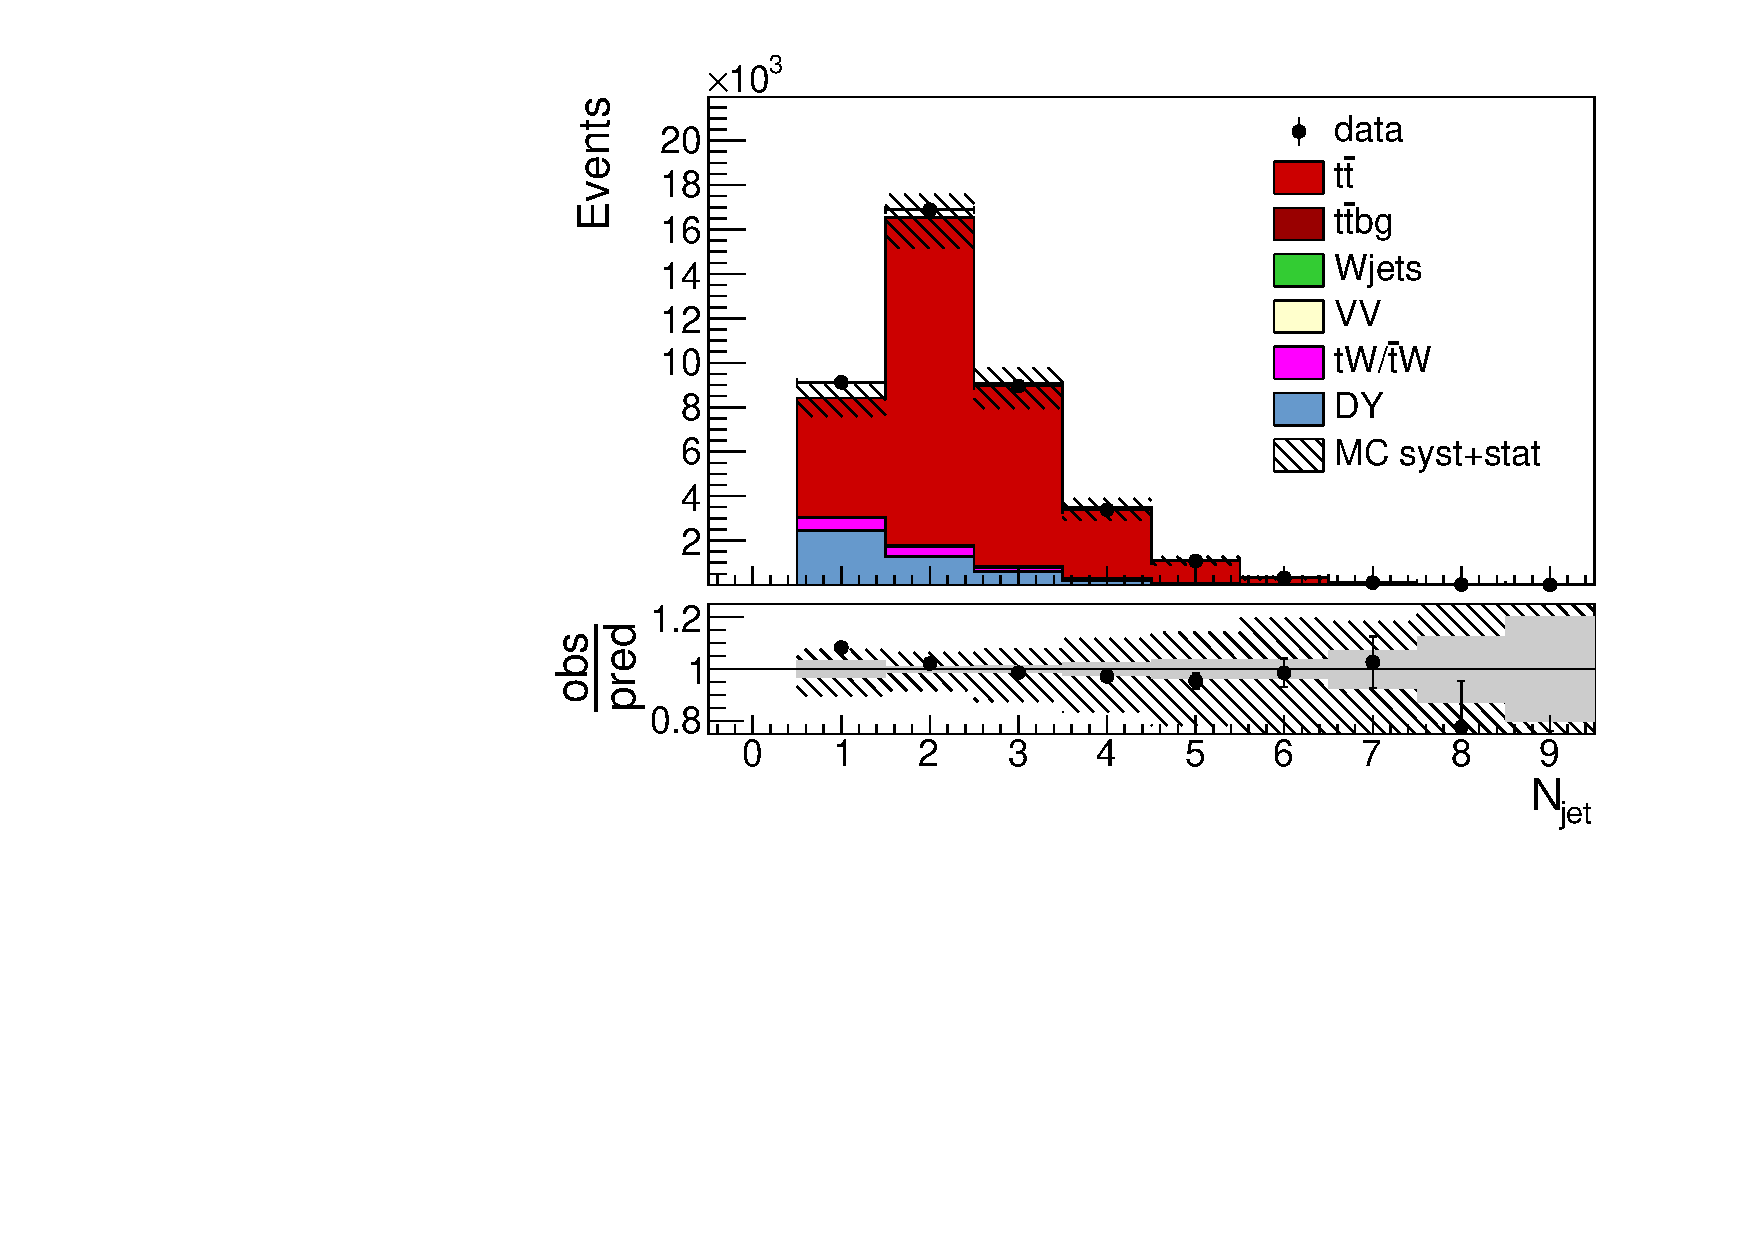
\includegraphics{CrossSection/Figures/ControlPlots/ee_sysnom/selected_jets_multi_step_8.pdf}}
    \resizebox{0.48 \textwidth}{!}{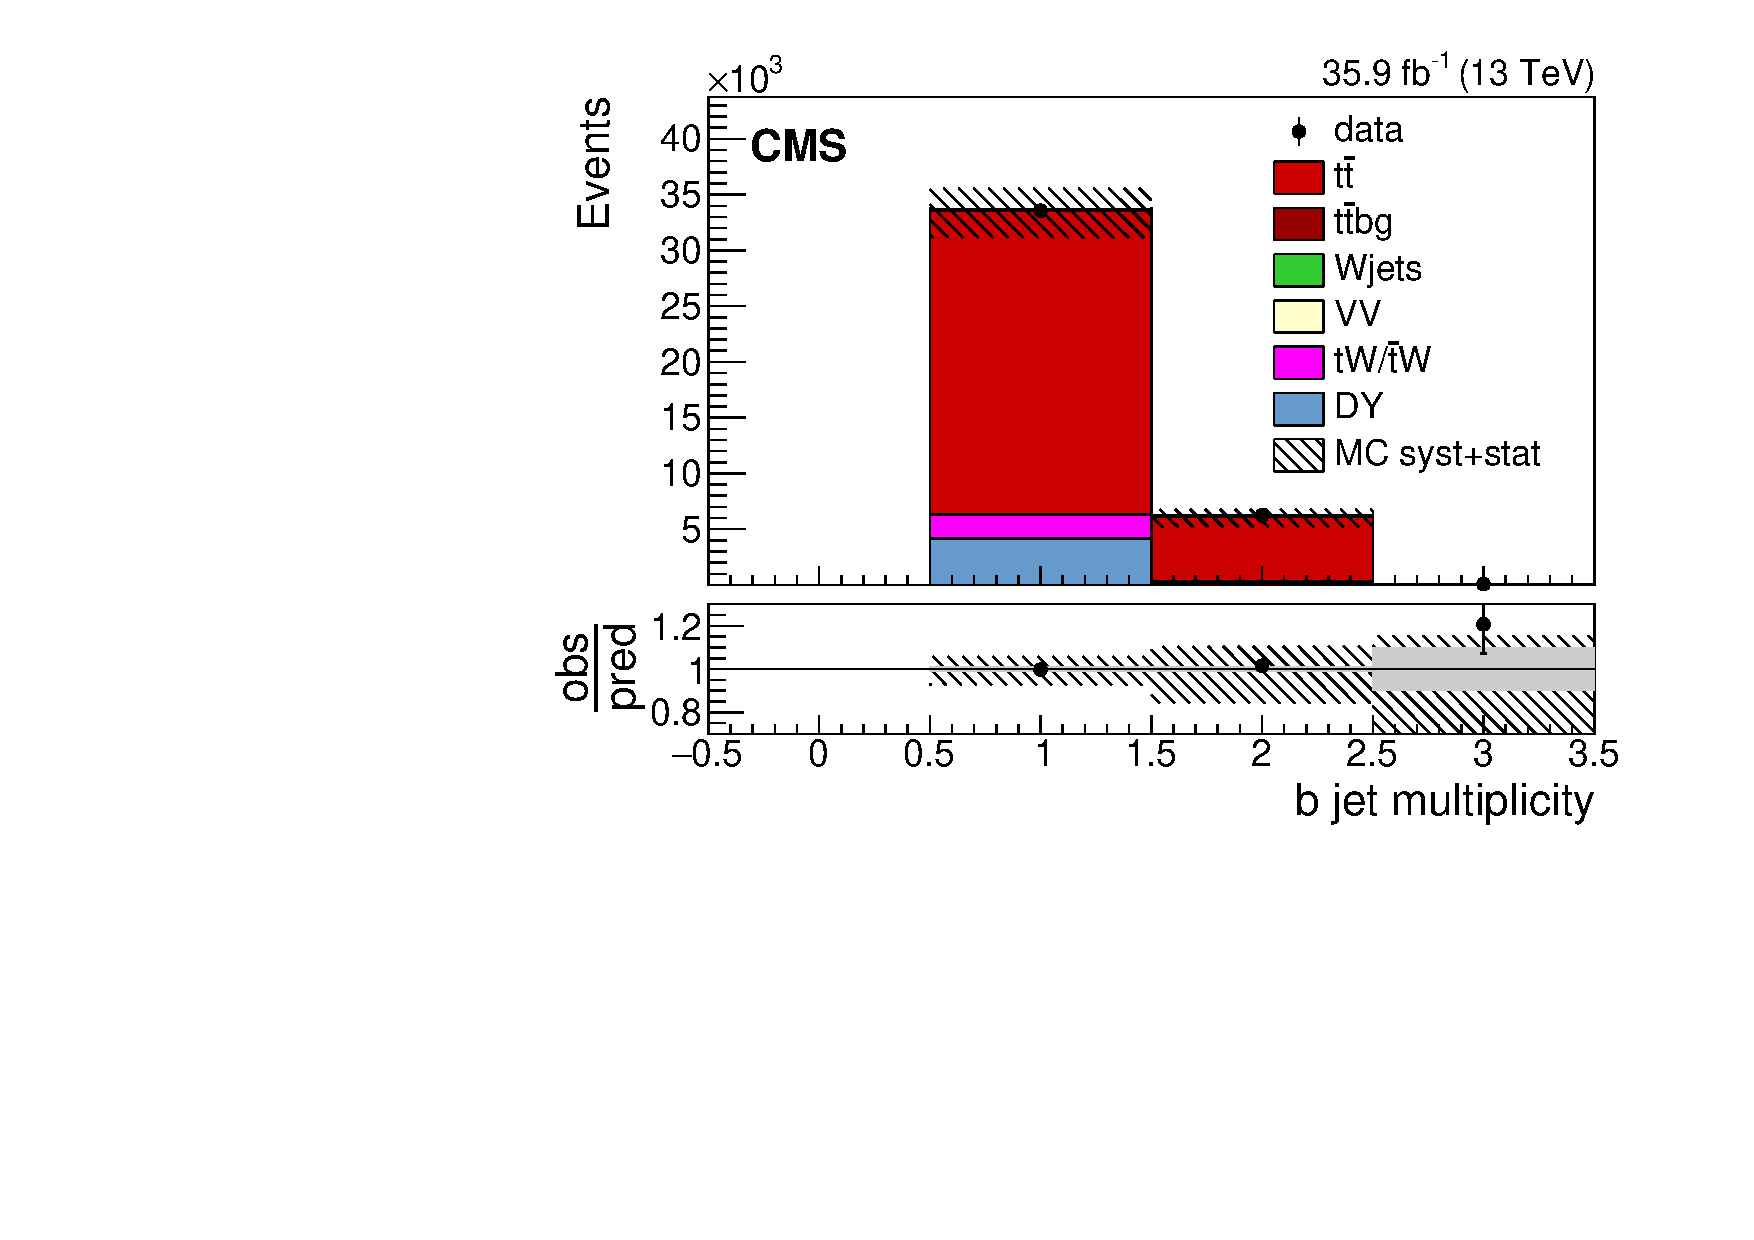
\includegraphics{CrossSection/Figures/ControlPlots/ee_sysnom/selected_b-jet_multi_step_8.pdf}}
      \caption{Transverse momentum (left) and pseudorapidity (right)
        of leading (first row) and second-leading (second row) lepton in the \ee channel after the
        event selection required by the \ttbar cross section
        extraction technique based on a simultaneous fit. Jet and b-jet multiplicity after the same selection steps are
        shown in the third row. The hatched
        bands correspond to the total uncertainty on the sum of the
        predicted yields. 
        %agrohsje , excluding luminosity and background
        %normalization uncertainties. 
        The ratios of data to the sum of the predicted yields are
        shown at the bottom of each plot. Here, the solid gray band
        represents the contribution of the statistical uncertainty.}  
       \label{fig:xsec_ee_ctrplots}
  \end{center}
\end{figure}

As described in Section \todo{Ref to reconstruction} the efficiency for the reconstruction of physics objects is different in data and simulation. This difference needs to be corrected in simulation.
This is especially important for leptons since we require two of those in the selection.
In order to assess the quality of the correction a carefull look into sensitive variables is important. Any large discrepancies between simulation and prediction would suggest that these corrections
are not optimal for the given selection.
The invariant mass of the dilepton system is shown in Figure \ref{fig:xsec_ctrplots_mll} for all three decay channels and depending on the number of b-tagged jets.
The simulation agrees with the measurement, so it can be assumed that the efficiency corrections are accurate.
The figures also show again how the DY contribution decreases when more b-tagged jets are required.


\begin{figure}[htbp!]
  \begin{center}
    \resizebox{0.48 \textwidth}{!}{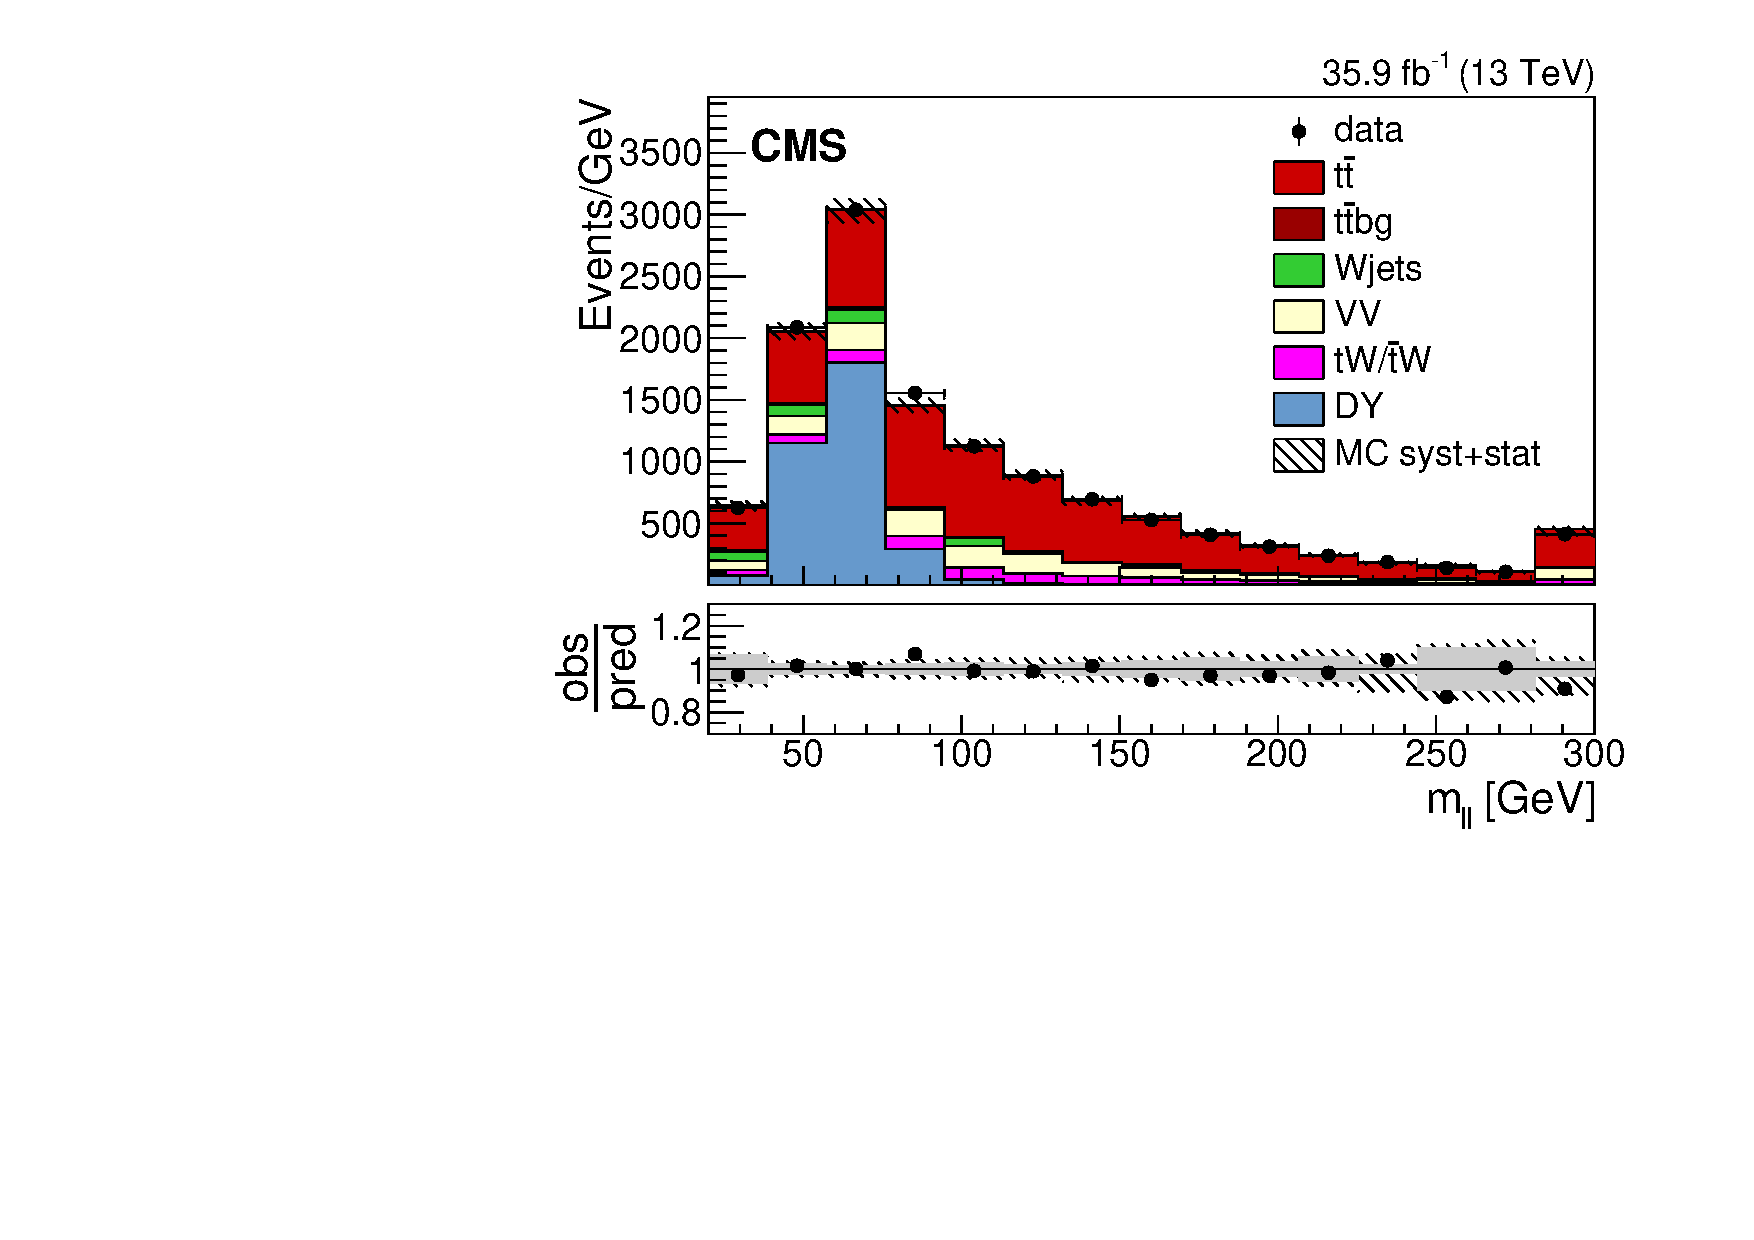
\includegraphics{CrossSection/Figures/ControlPlots/emu_sysnom/mll_0_b-jets_step_8.pdf}}
    \resizebox{0.48 \textwidth}{!}{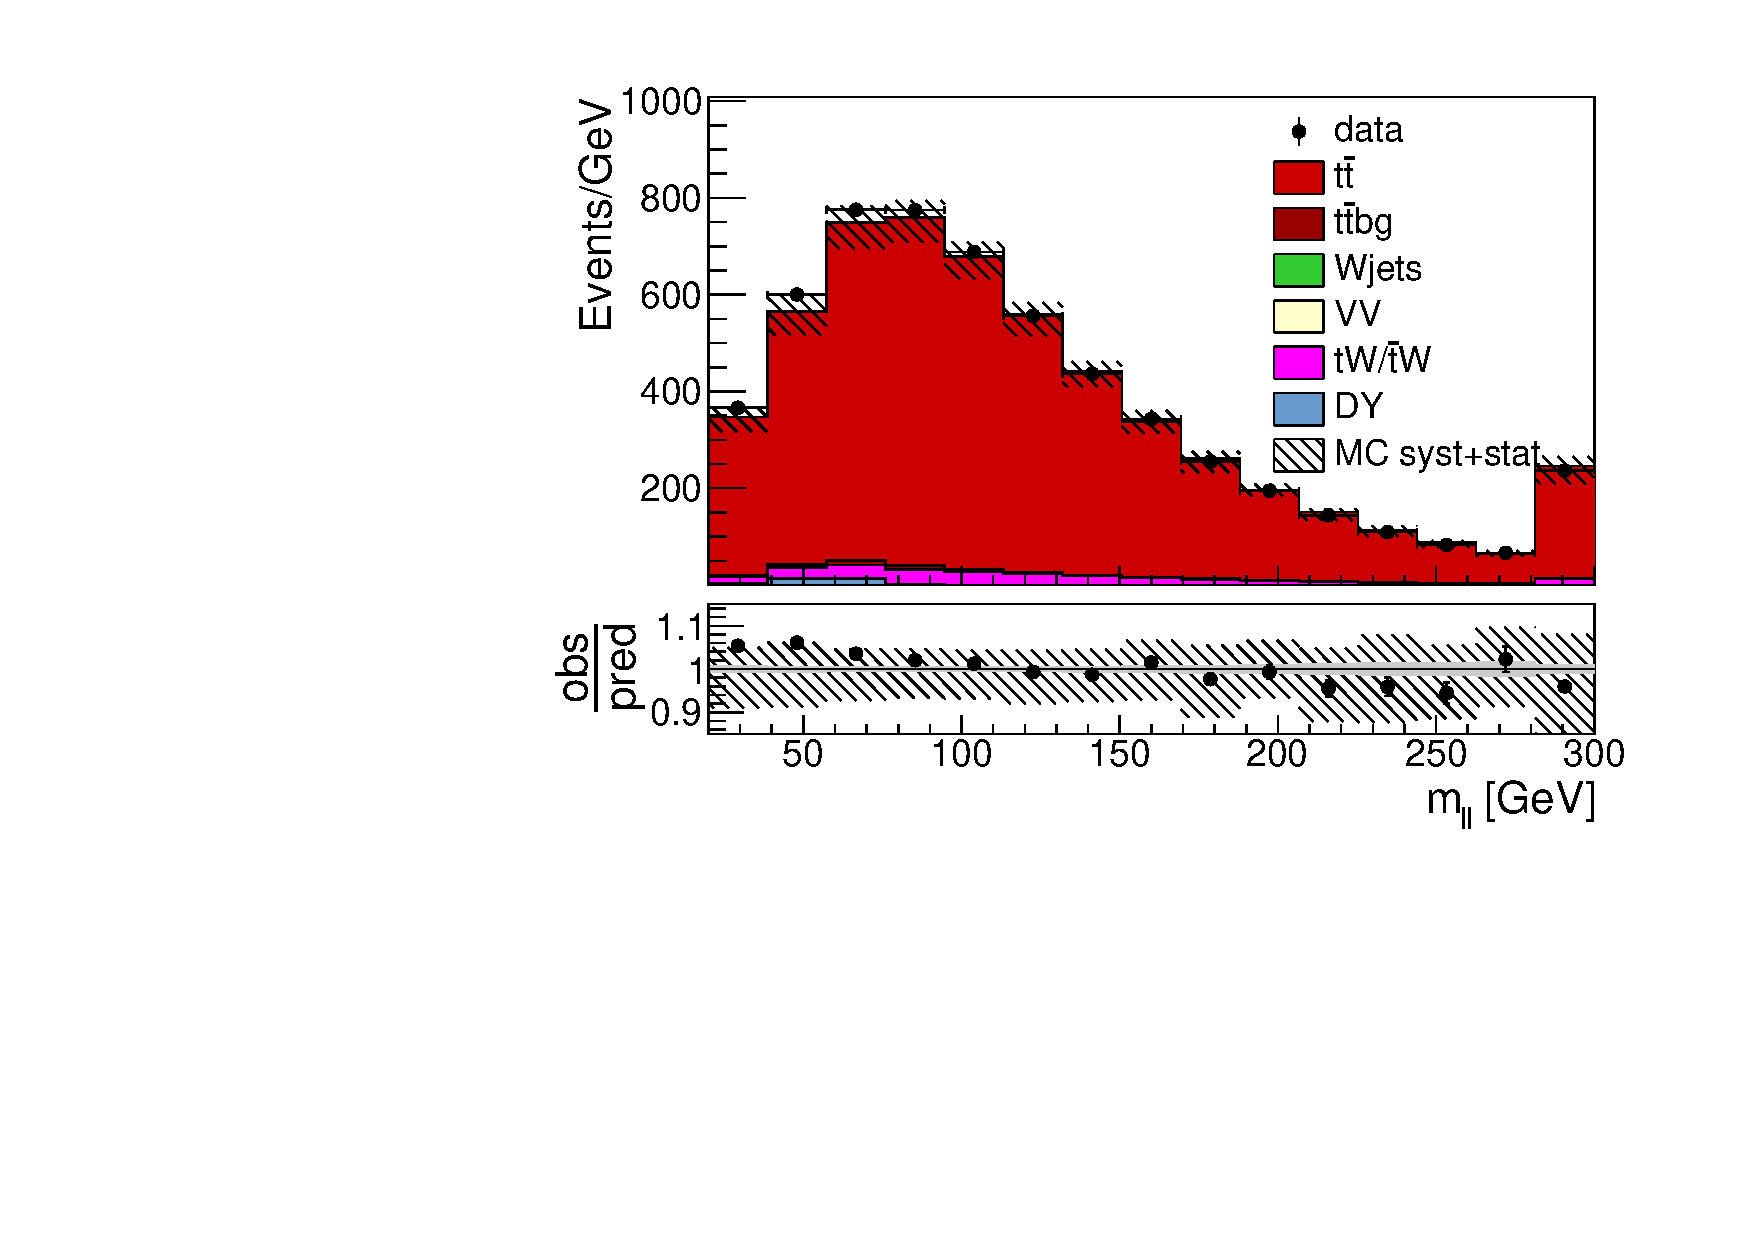
\includegraphics{CrossSection/Figures/ControlPlots/emu_sysnom/mll_1_b-jets_step_8.pdf}}
    \resizebox{0.48 \textwidth}{!}{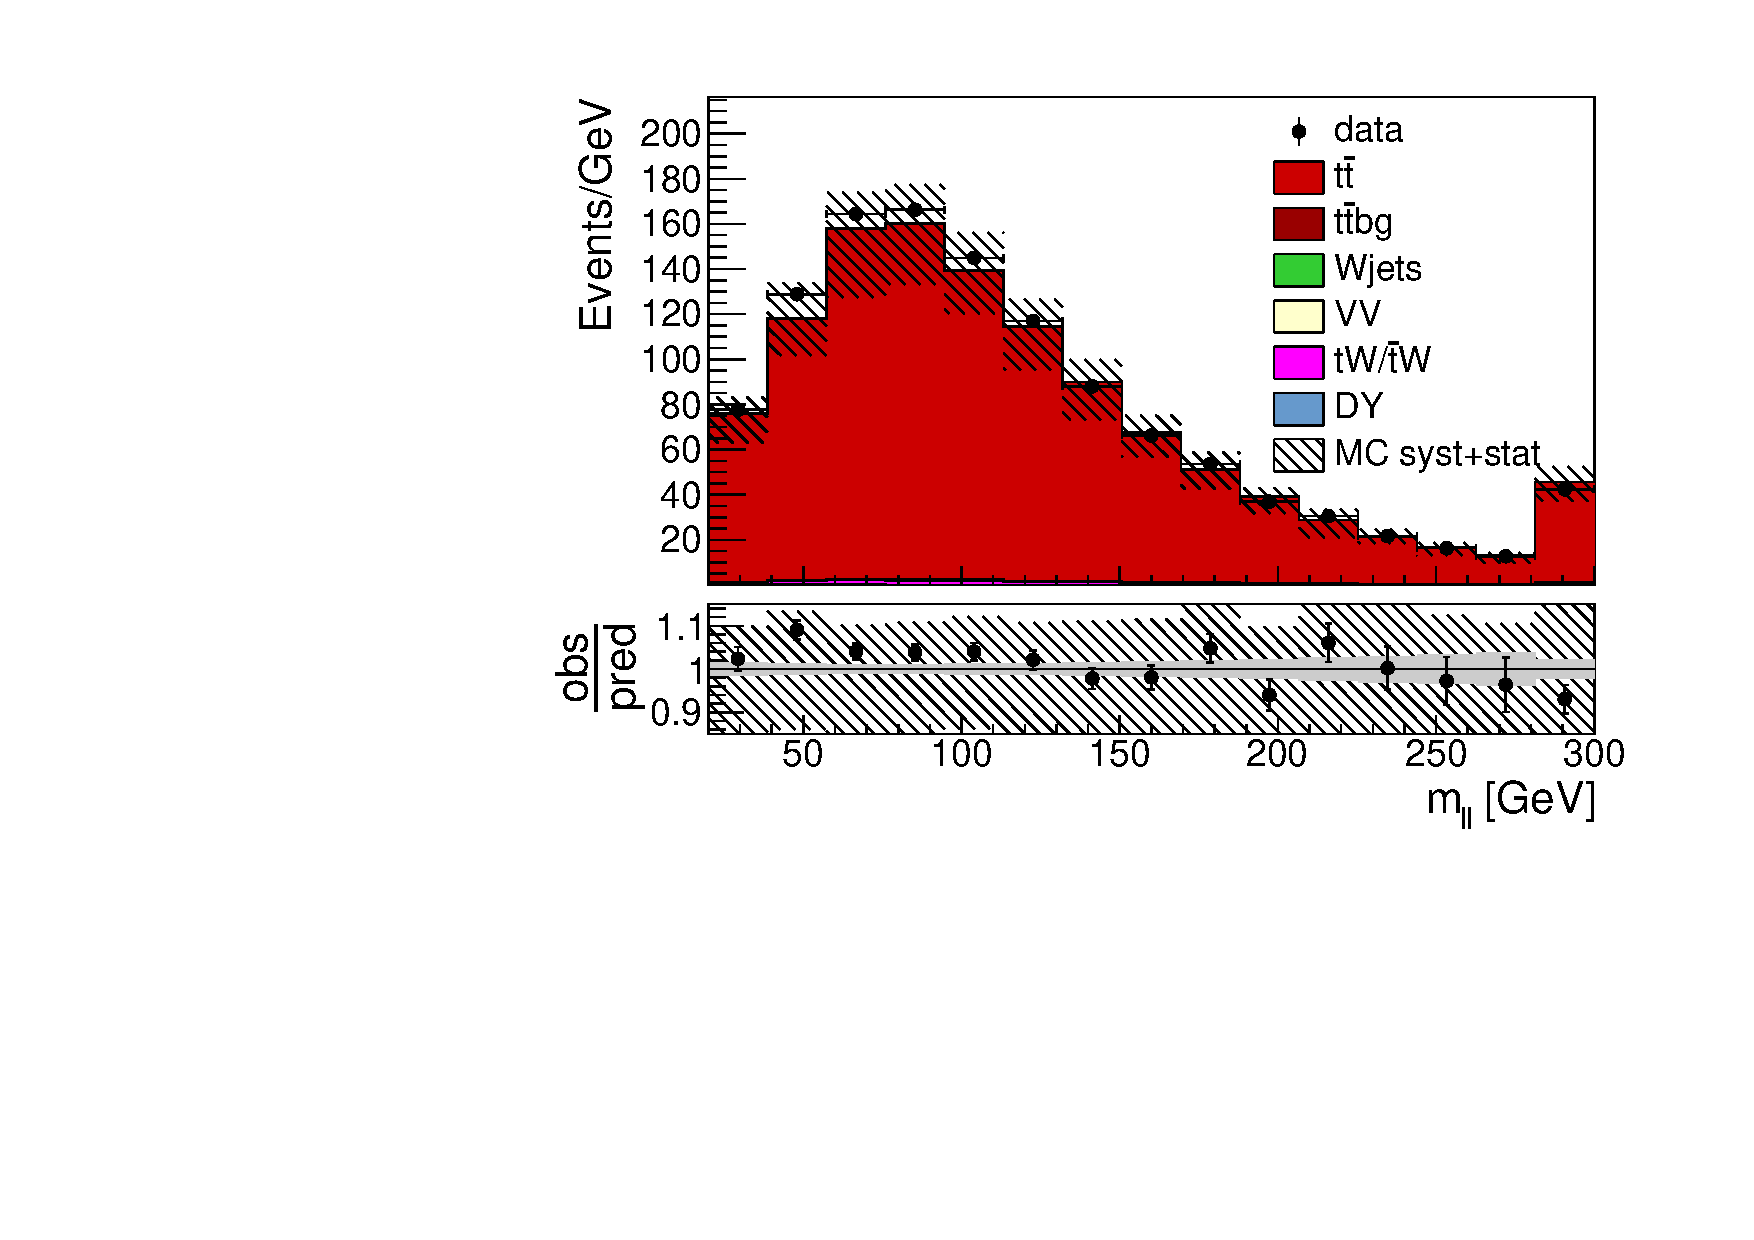
\includegraphics{CrossSection/Figures/ControlPlots/emu_sysnom/mll_2_b-jets_step_8.pdf}} \\
        \resizebox{0.48 \textwidth}{!}{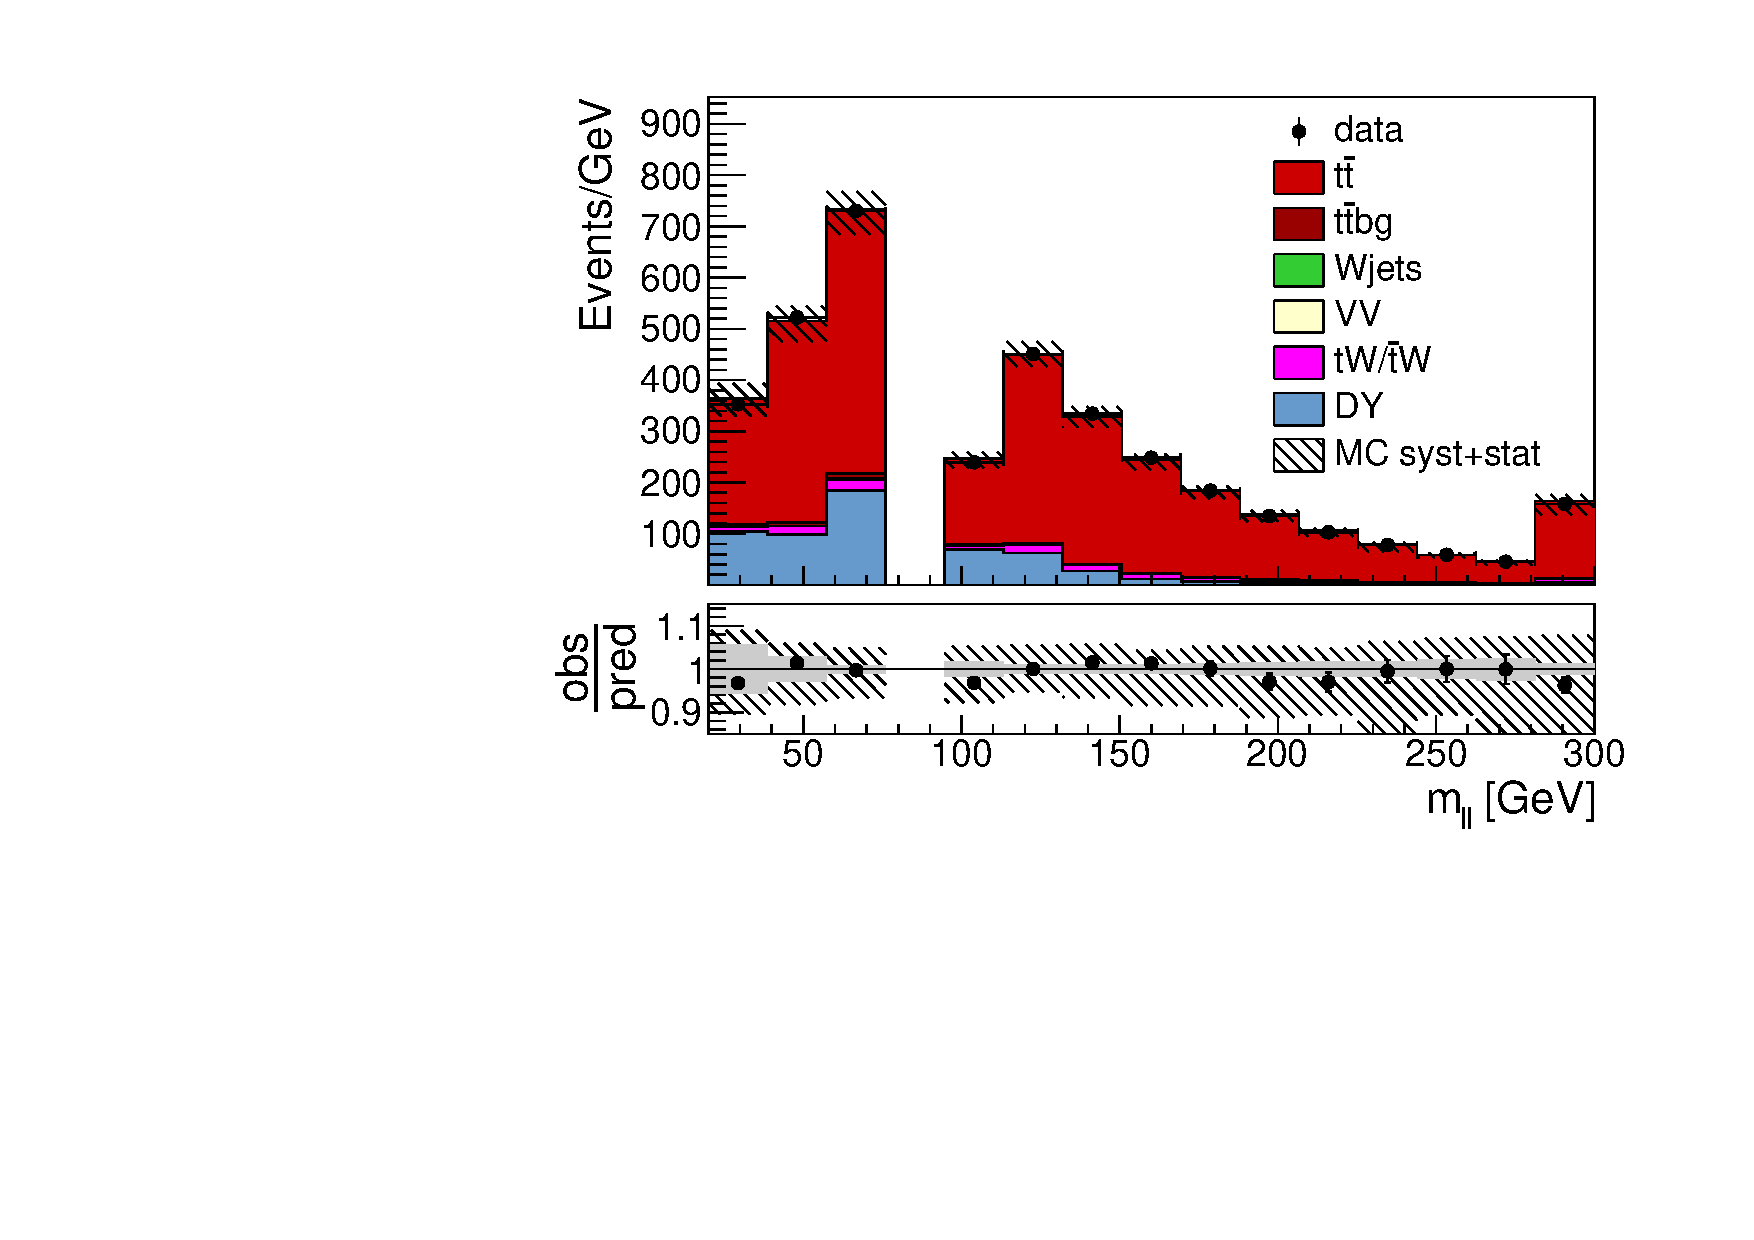
\includegraphics{CrossSection/Figures/ControlPlots/mumu_sysnom/mll_1_b-jets_step_8.pdf}}
    \resizebox{0.48 \textwidth}{!}{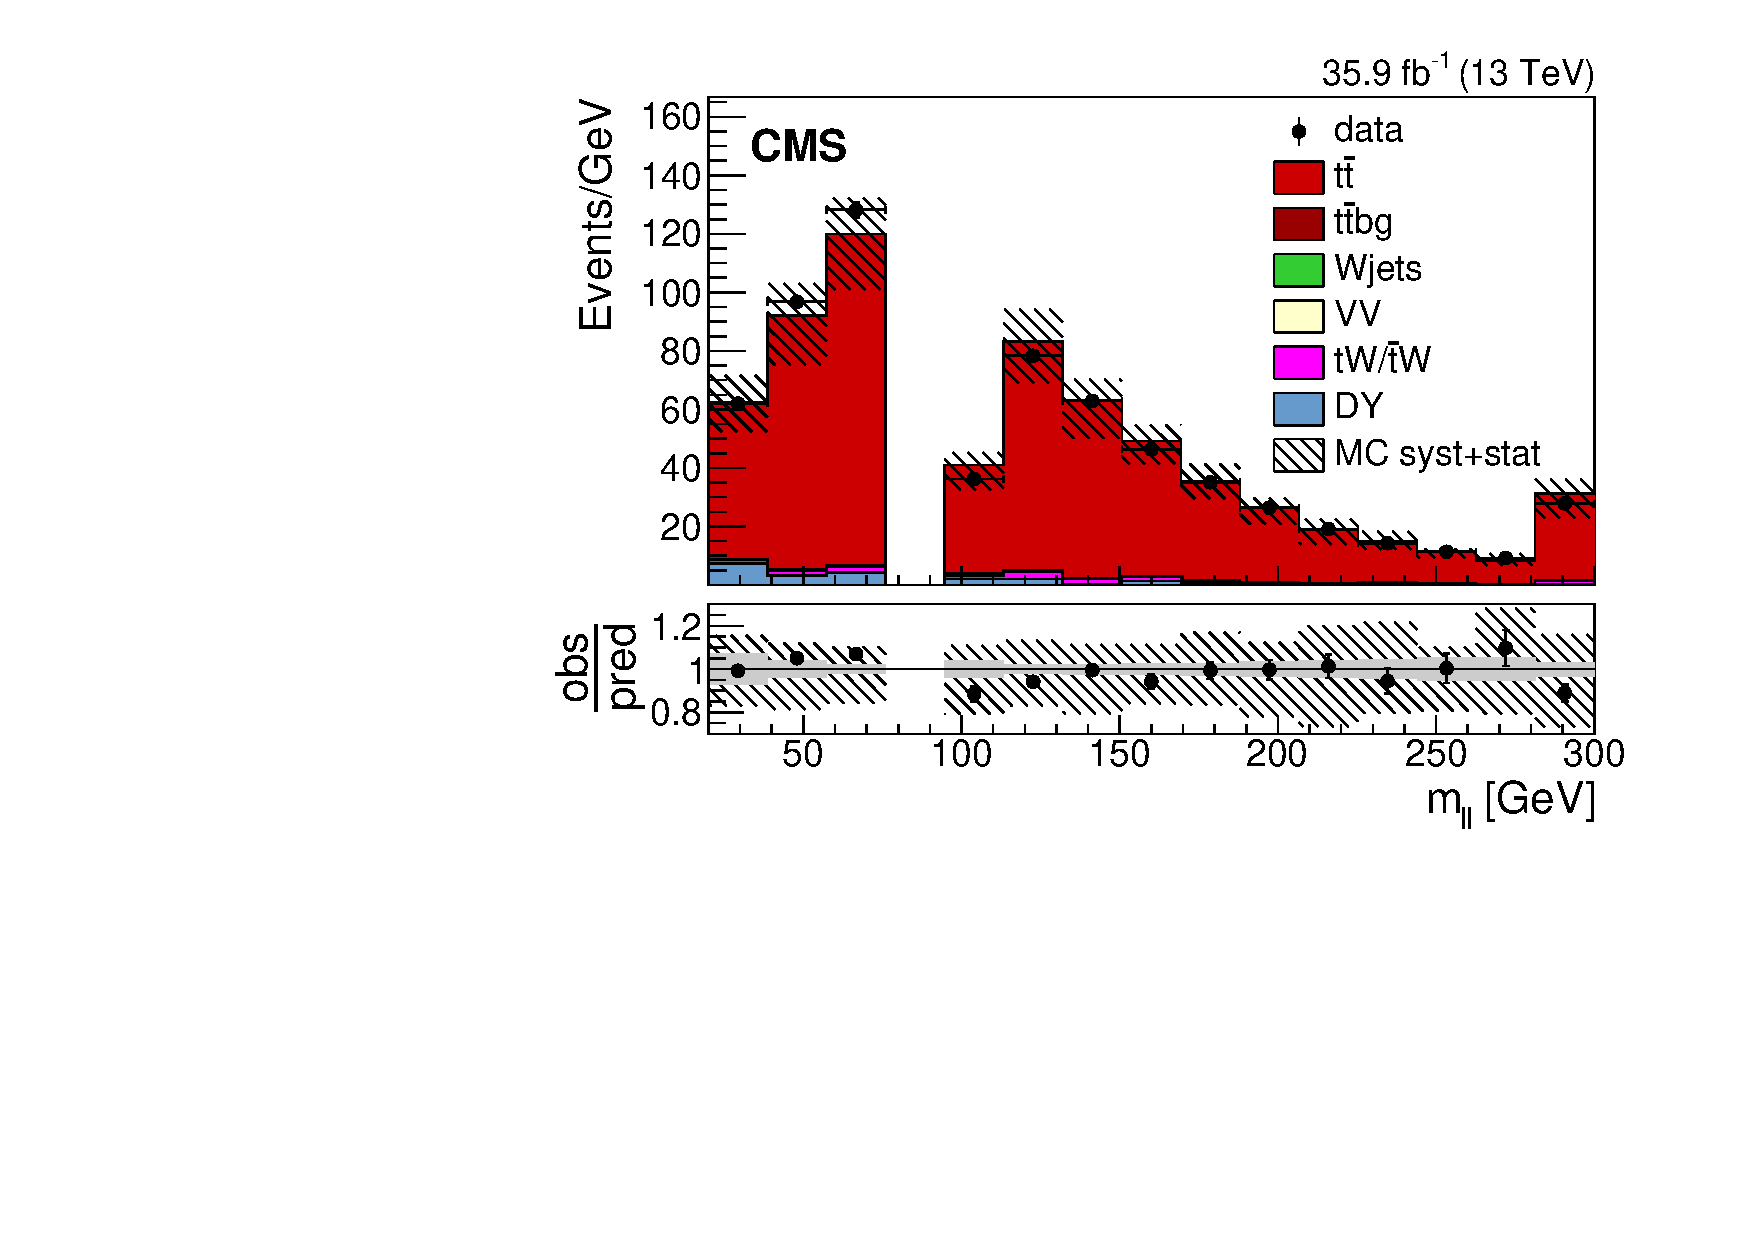
\includegraphics{CrossSection/Figures/ControlPlots/mumu_sysnom/mll_2_b-jets_step_8.pdf}} \\
        \resizebox{0.48 \textwidth}{!}{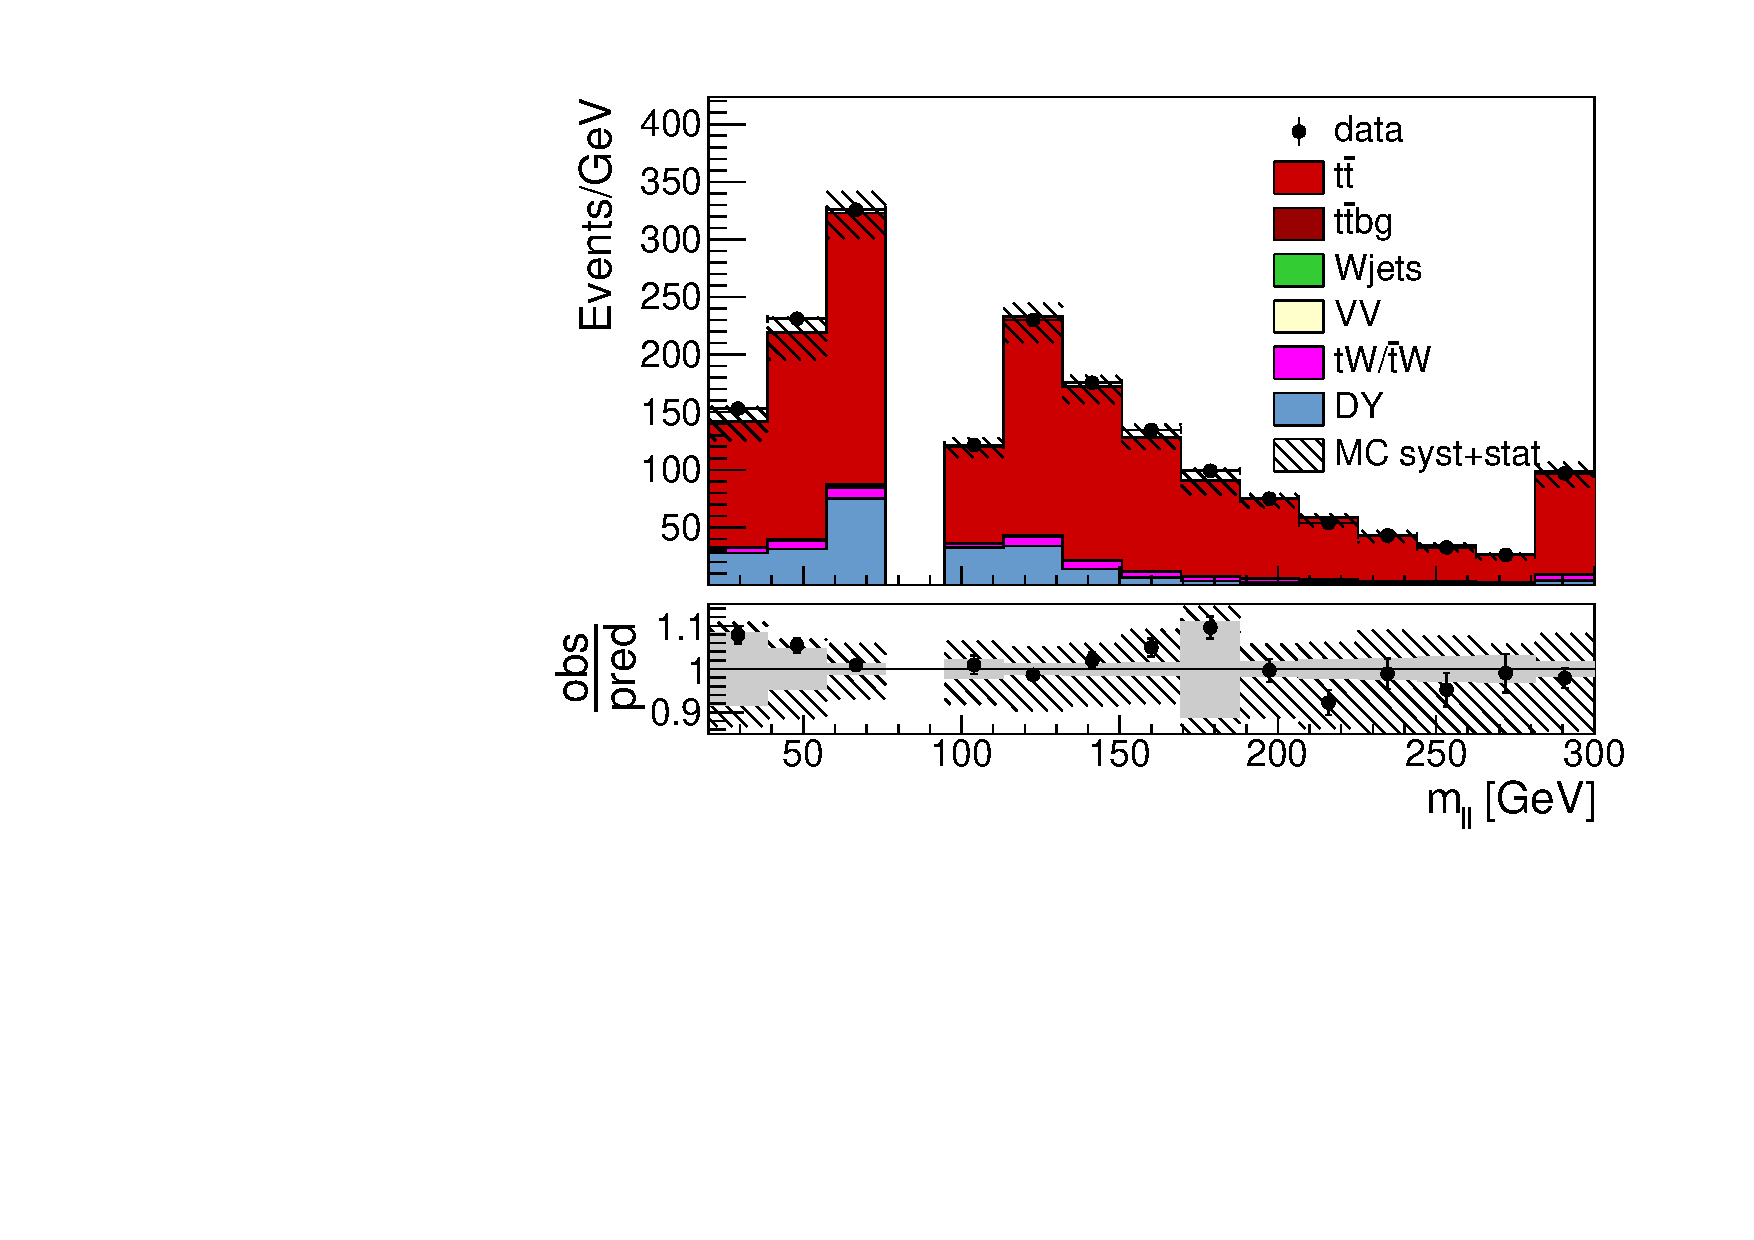
\includegraphics{CrossSection/Figures/ControlPlots/ee_sysnom/mll_1_b-jets_step_8.pdf}}
    \resizebox{0.48 \textwidth}{!}{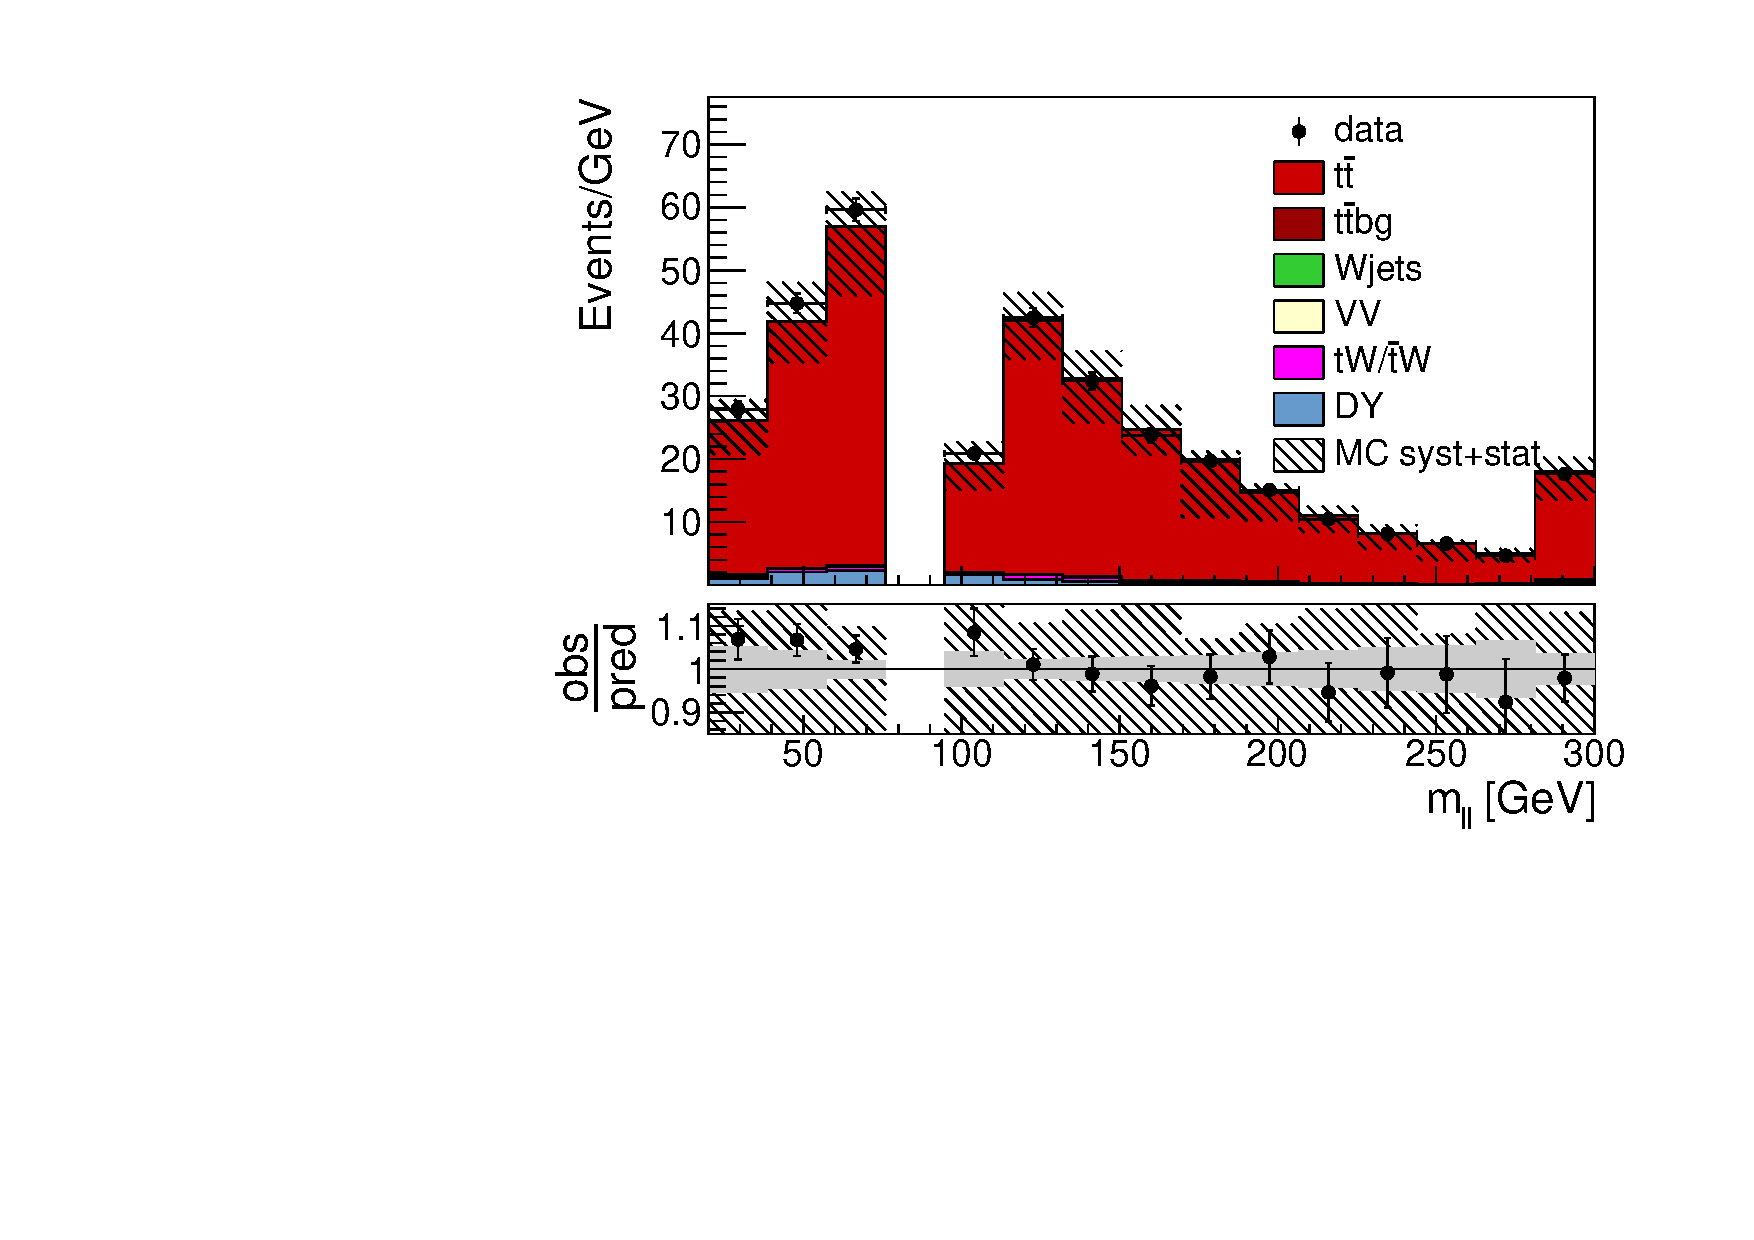
\includegraphics{CrossSection/Figures/ControlPlots/ee_sysnom/mll_2_b-jets_step_8.pdf}}

      \caption{Invariant mass of the dilepton system with zero (top row left), one (top row right) and two (second row) b-tagged 
      jets in the \emu channel. The invariant mass of the dilepton system in the \mumu (third row) and \ee (bottom row) with one (left)
      and two b-tagged jets (right).
        %agrohsje , excluding luminosity and background
        %normalization uncertainties. 
        The ratios of data to the sum of the predicted yields are
        shown at the bottom of each plot. Here, the solid gray band
        represents the contribution of the statistical uncertainty.}  
       \label{fig:xsec_ctrplots_mll}
  \end{center}
\end{figure}


\section{Extracting the Cross Section}
\label{sec:xsec_fit}

As given in Equation \ref{eq:CaC} the cross section depends mainly on three variables, $N_{top}$,$\varepsilon$, $A$, while the luminosity is given by a different measurement.
These three quantities have to be determined in order to measure the cross section. 

Here, this is done with a binned $\chi^2$ fit where the templates for \ttbar and background events taken from simulation are fitted to data distributions and systematic uncertainties are treated as nuisance parameters.
This allows to reduce the impact of the systematic uncertainties on the cross section measurement, depending on the choice of templates and event classification.

The acceptance is defined as the fraction of the visible to the full phase space (see Section \ref{sec:xsec_sel} for the definition of the visible phase space).
Since the measurement can only be done in the visible phase space this value has to be taken from simulation and it can only be constrained within the visible phase space.

The nominal value for the efficiency is taken from simulation as well.  But here, the simulation has been corrected for the efficiency in data as explained in \todo{Link to SFs}. 
As the efficiency for all selected physics objects has been measured in data the efficiency value from simulation corresponds to the efficiency in data within the uncertainties.

The templates for the fit are separated first separated according to the dilepton decay channel. Since the efficiencies for the muon and electron reconstruction are correlated in all the channels and the \emu channel depends on both this separation allows to constrain the higher of the two lepton related uncertainties.

In order to further increase the separation between signal and background the events are further divided according to the number of b-tagged jets.
There are three categories of events with one, two and zero or more than two b-tagged jets.

This allows an explicit and independent determination of the efficiency of the b-tagging algorithm for data and simulation depending on the nuisance parameters. The efficiency of the b-tagging algorithm should be independent of the rest of the event, so it can be assumed to be the same in all \ttbar decay channels.
This intrinsic measurement of the b-tagging efficiency in the phase space of the measurement is also expected to reduce the impact of the uncertainties on the b-tagging efficiency on the final measurement of the \ttbar cross section.


\subsection{The Choice of Sensitive Templates}
\label{sec:xsec_templates}

The choice of templates is an important part of the fitting procedure.
The variables that are used should both allow to further separate signal and background processes and at the same time be sensitive to systematic
variations in order to constrain their impact on the final result.

As the b-tagging efficiency is already determined intrinsically the fit will already be sensitive to the related nuisance parameters.
Beside the number of b-jets, the number of light jets is one of the main discriminators between \ttbar and background events.
Together with the \pt of the light jets it is also sensitive to the systematic uncertainty on the response of the jet reconstruction and
the systematic uncertainties introduced by theoretical assumptions in the simulation.
These systematic uncertainties make large contributions to the total uncertainty on the \ttbar cross section measurement \todo{Link to CC}, so reducing them is important.

The final templates are shown in Figures \ref{fig:xsec_emu_inputdistr,fig:xsec_mumu_inputdistr,fig:xsec_ee_inputdistr} for the \emu,\mumu and \ee channel respectively. The events are divided first by the dilepton decay channel, then by number of b-tagged jets and 
then by the number of additional light jets resulting in twenty eight distributions overall.

\begin{figure}[htbp!]
  \begin{center}
    \resizebox{0.24 \textwidth}{!}{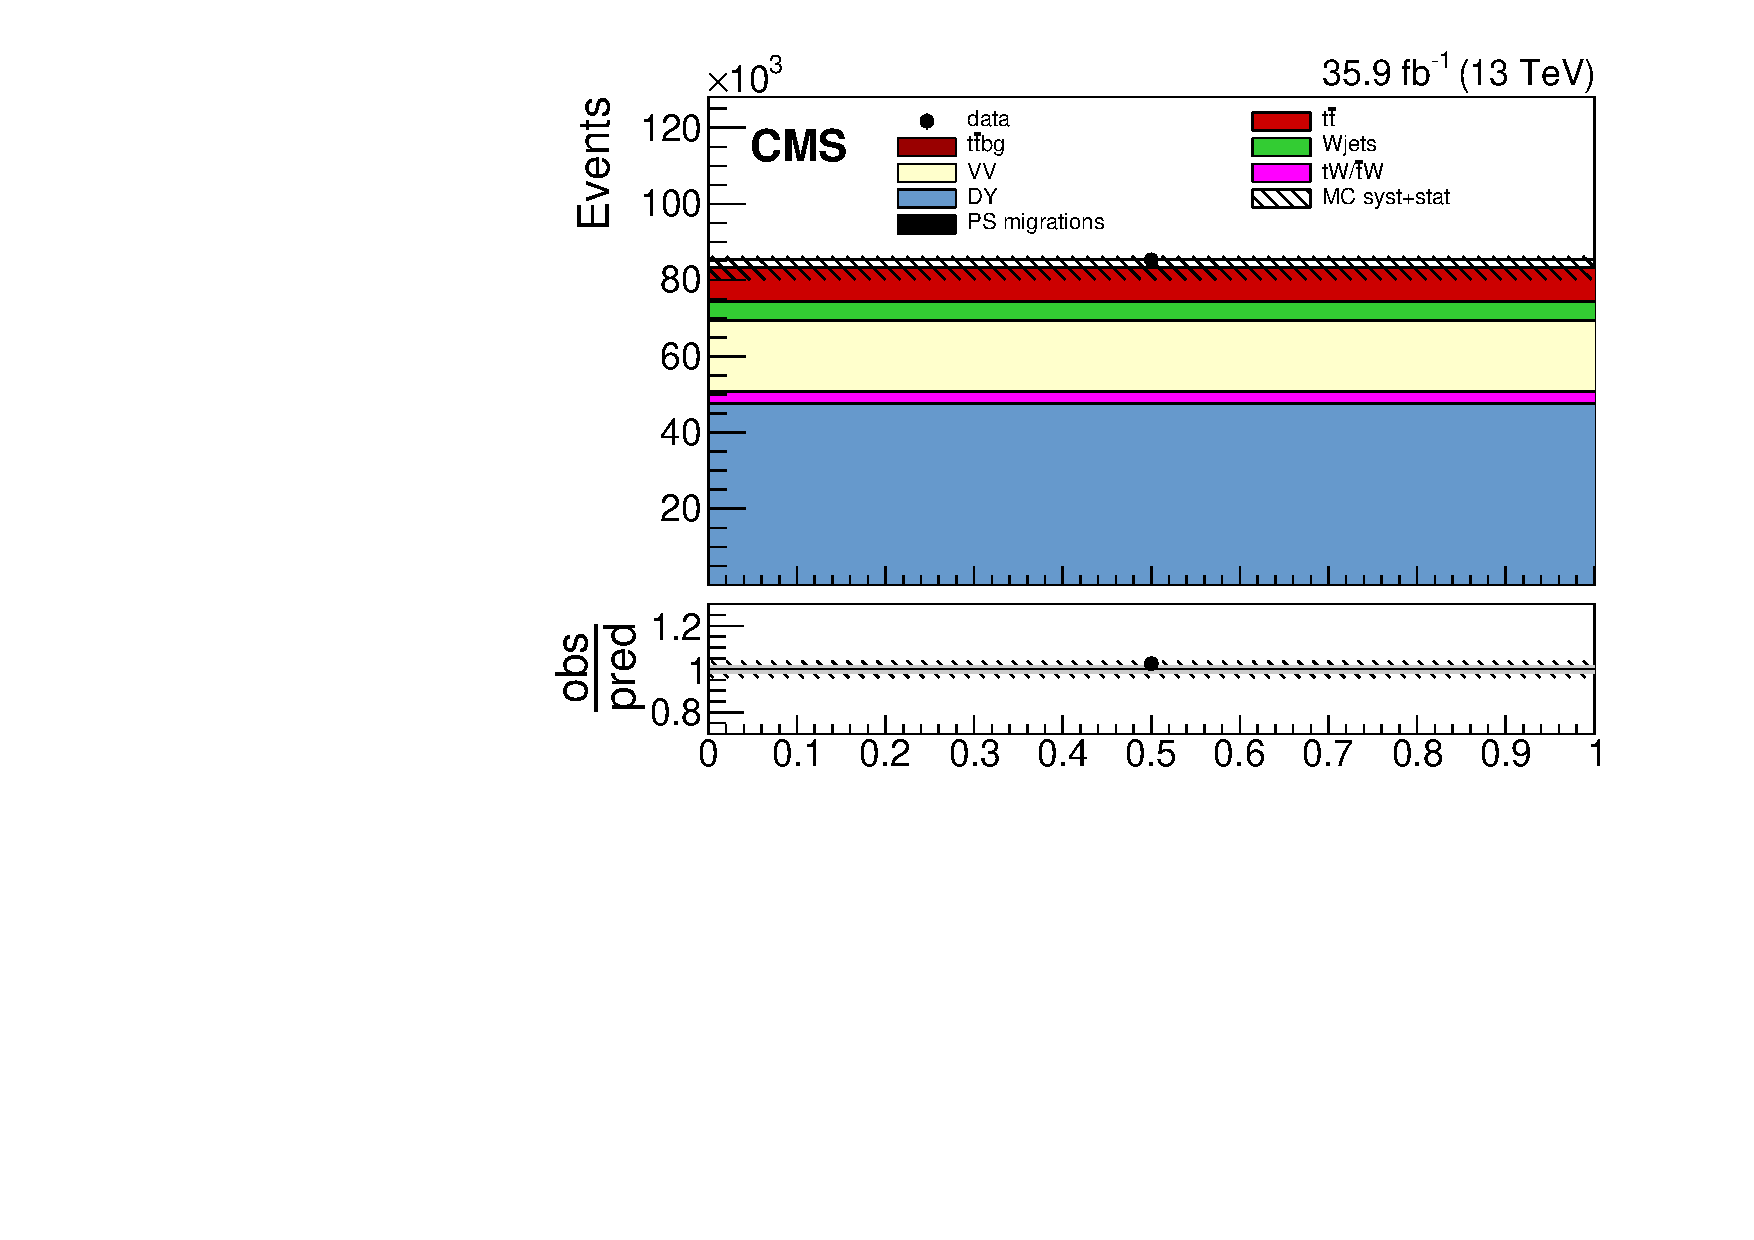
\includegraphics{CrossSection/Figures/ControlPlots/emu_sysnom/total_0_0_b-jets_step_8.pdf}}
    \resizebox{0.24 \textwidth}{!}{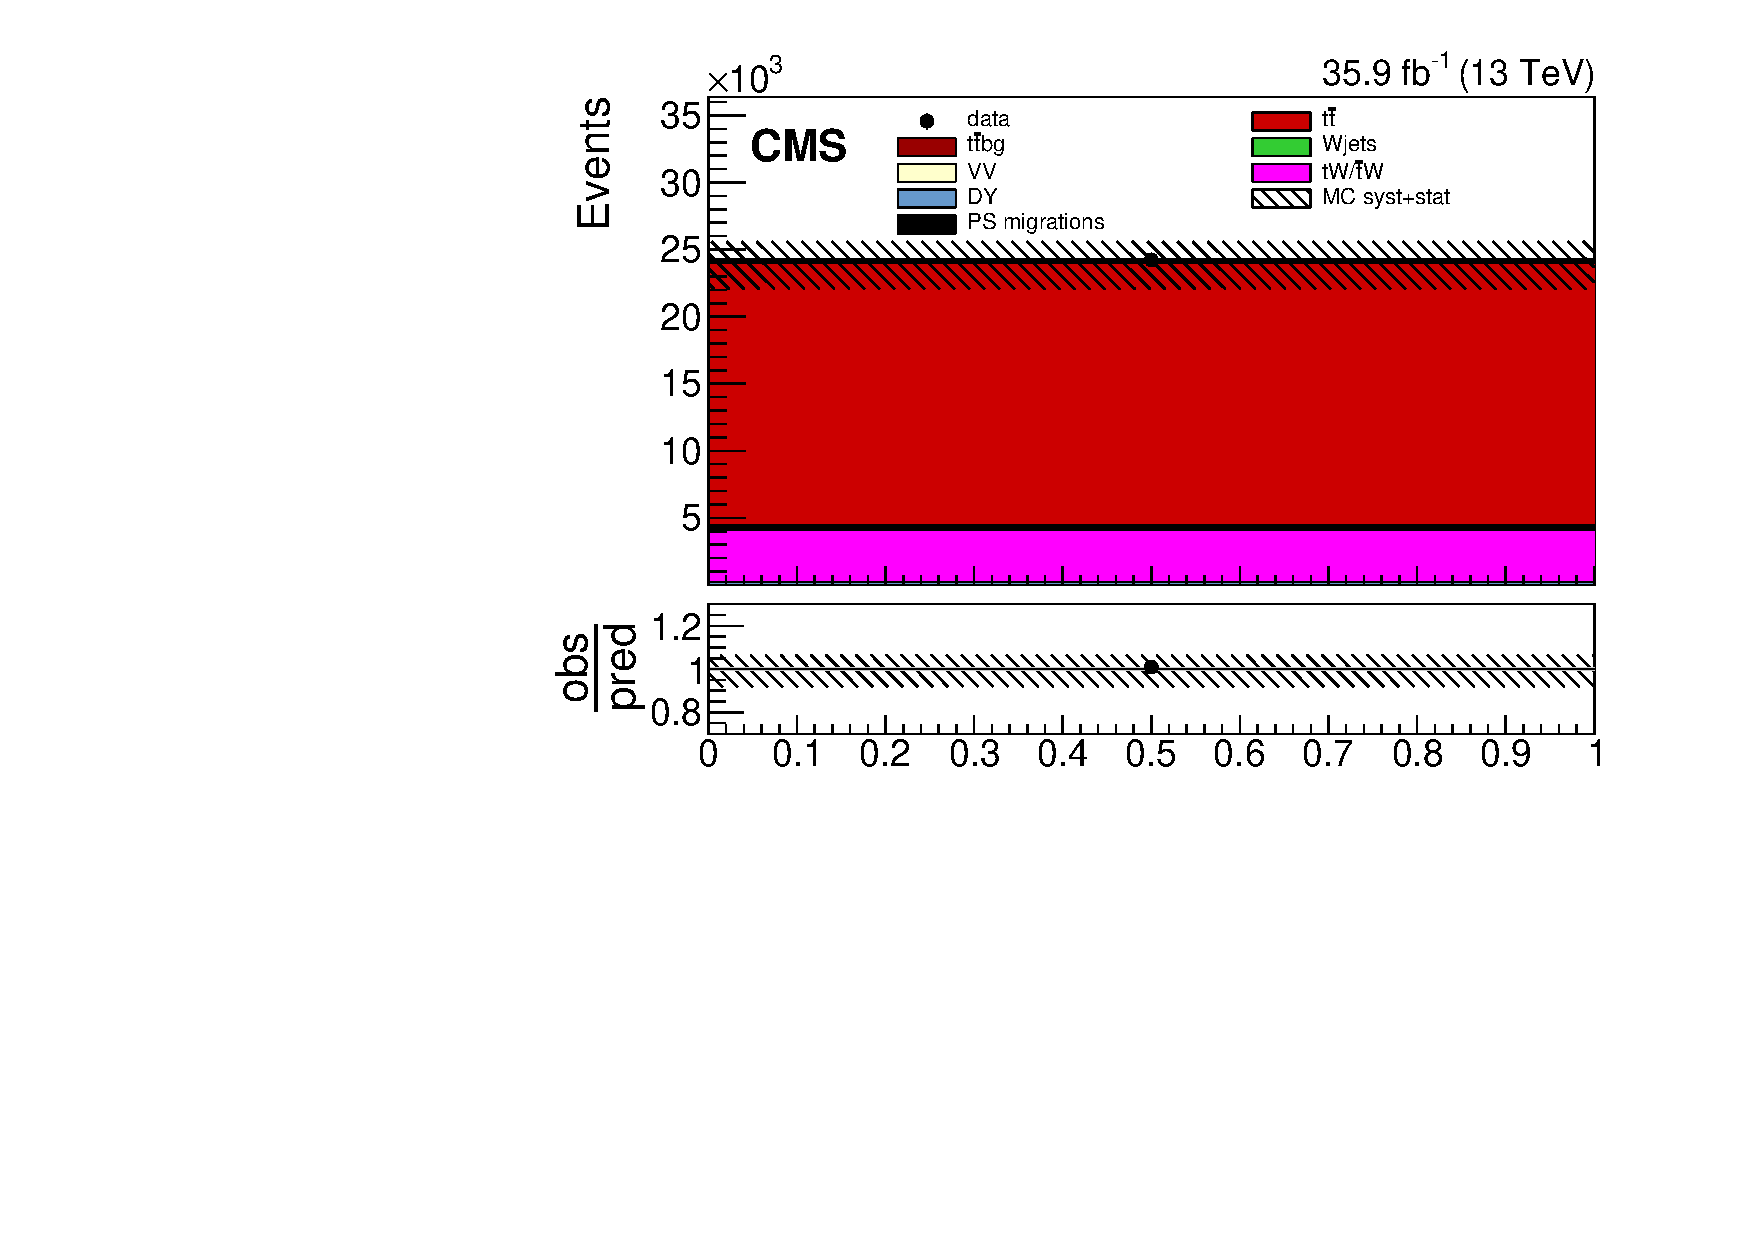
\includegraphics{CrossSection/Figures/ControlPlots/emu_sysnom/total_1_0_b-jets_step_8.pdf}}
    \resizebox{0.24 \textwidth}{!}{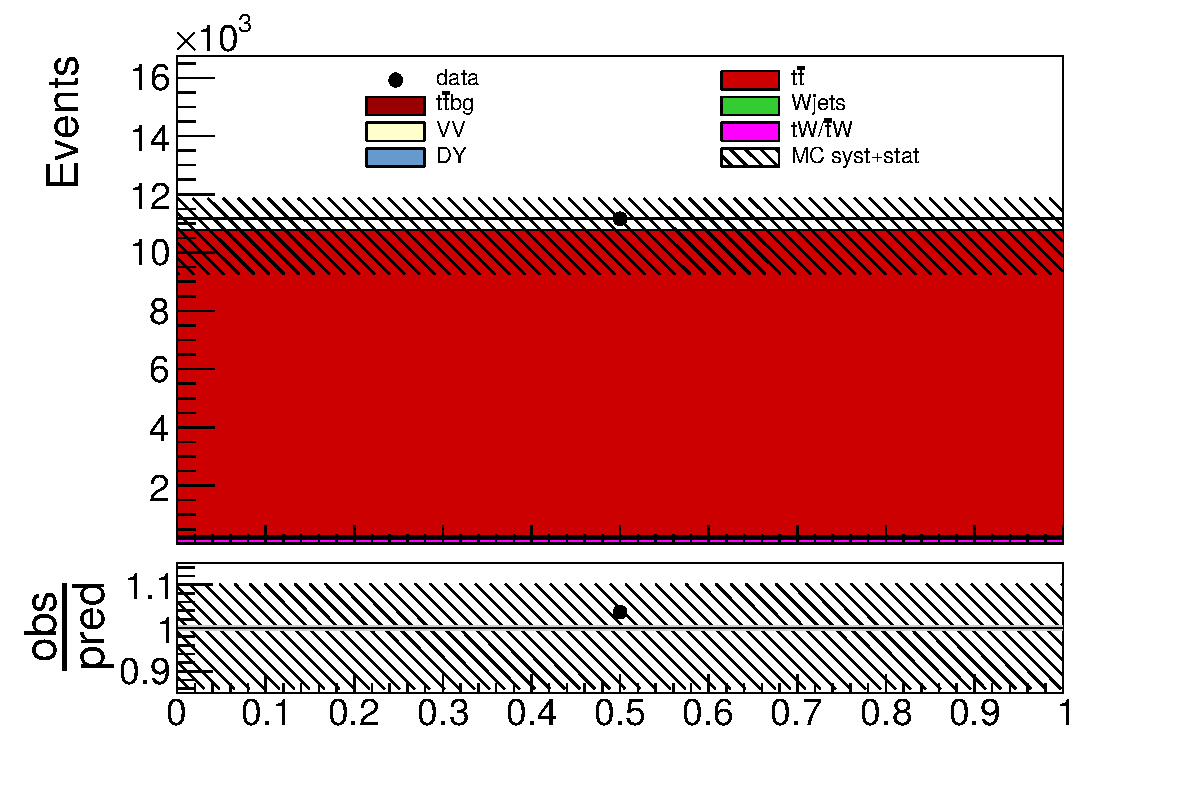
\includegraphics{CrossSection/Figures/ControlPlots/emu_sysnom/total_2_0_b-jets_step_8.pdf}}

    \resizebox{0.32 \textwidth}{!}{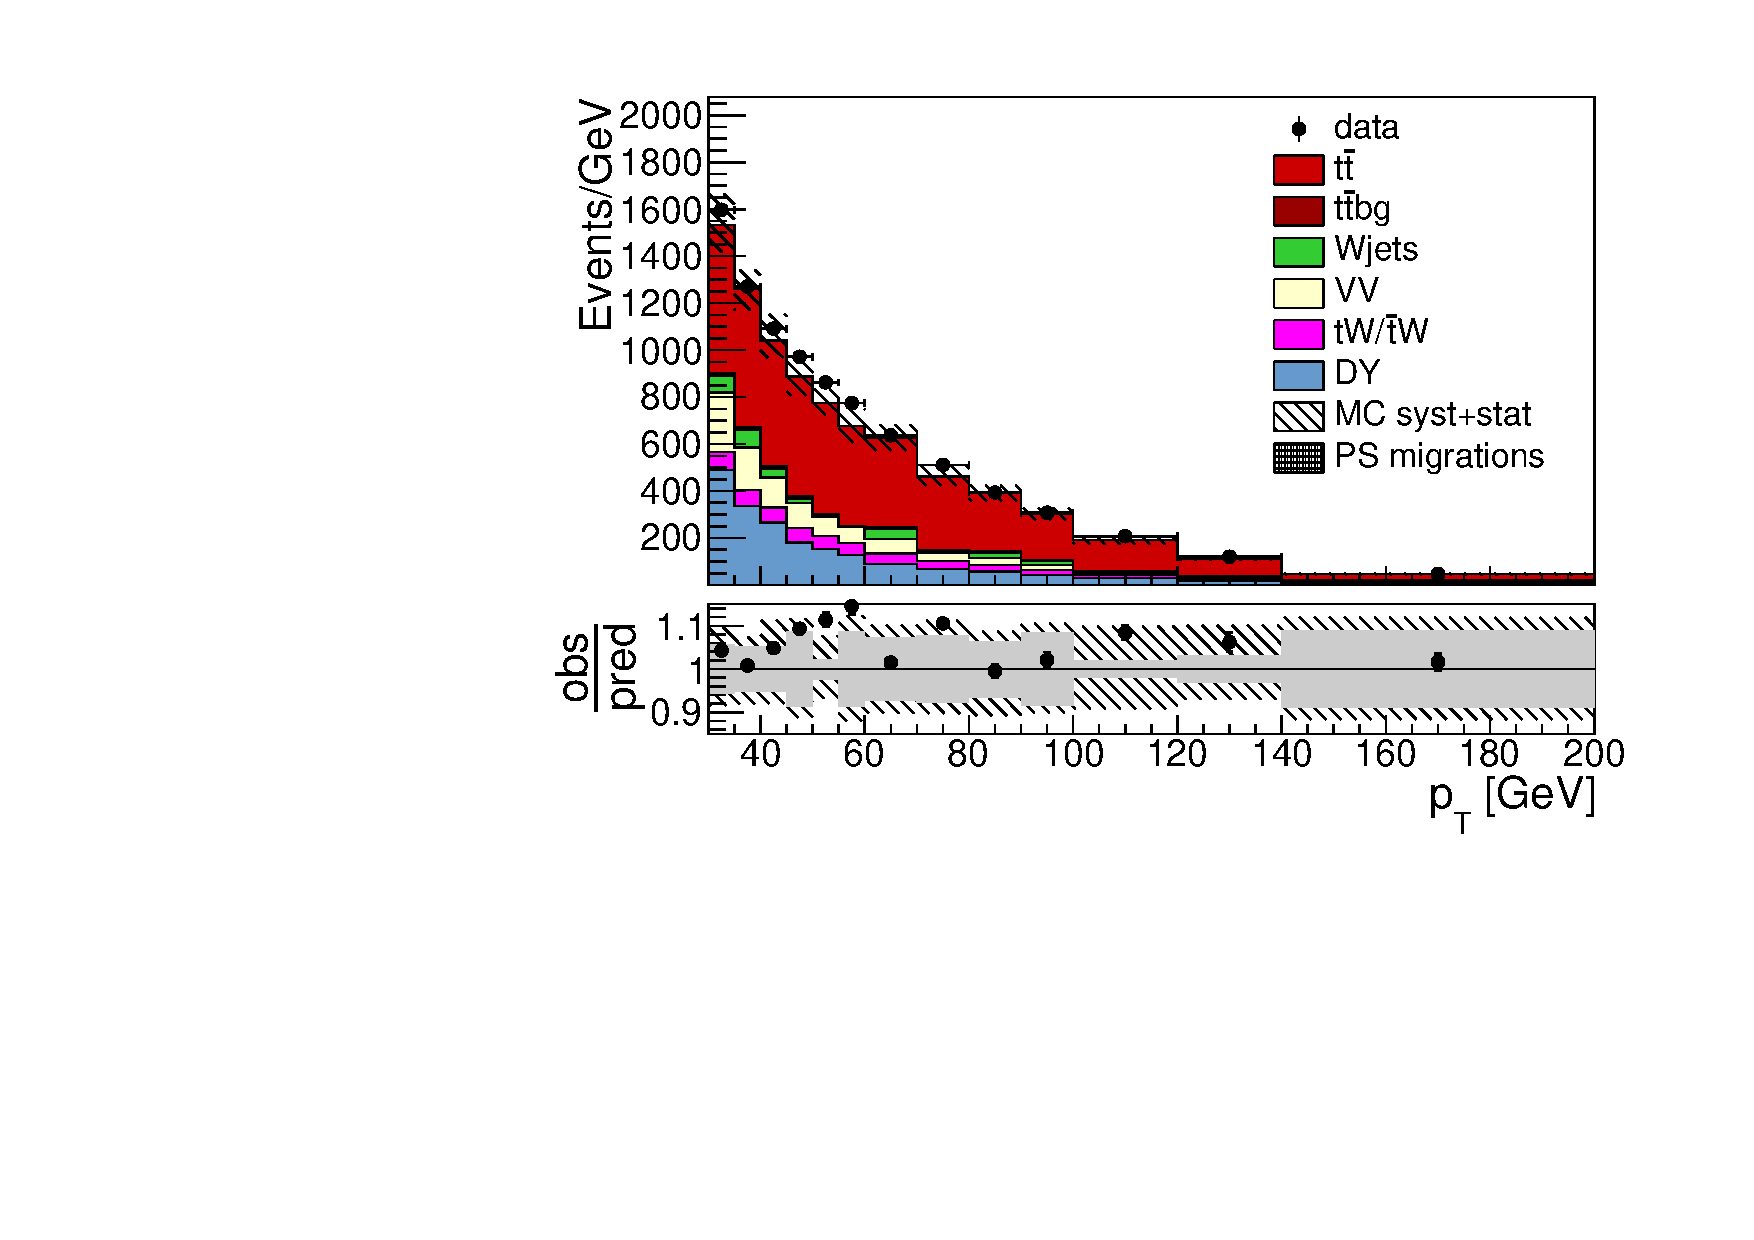
\includegraphics{CrossSection/Figures/ControlPlots/emu_sysnom/lead_jet_pt_0_1_b-jets_step_8.pdf}}
    \resizebox{0.32 \textwidth}{!}{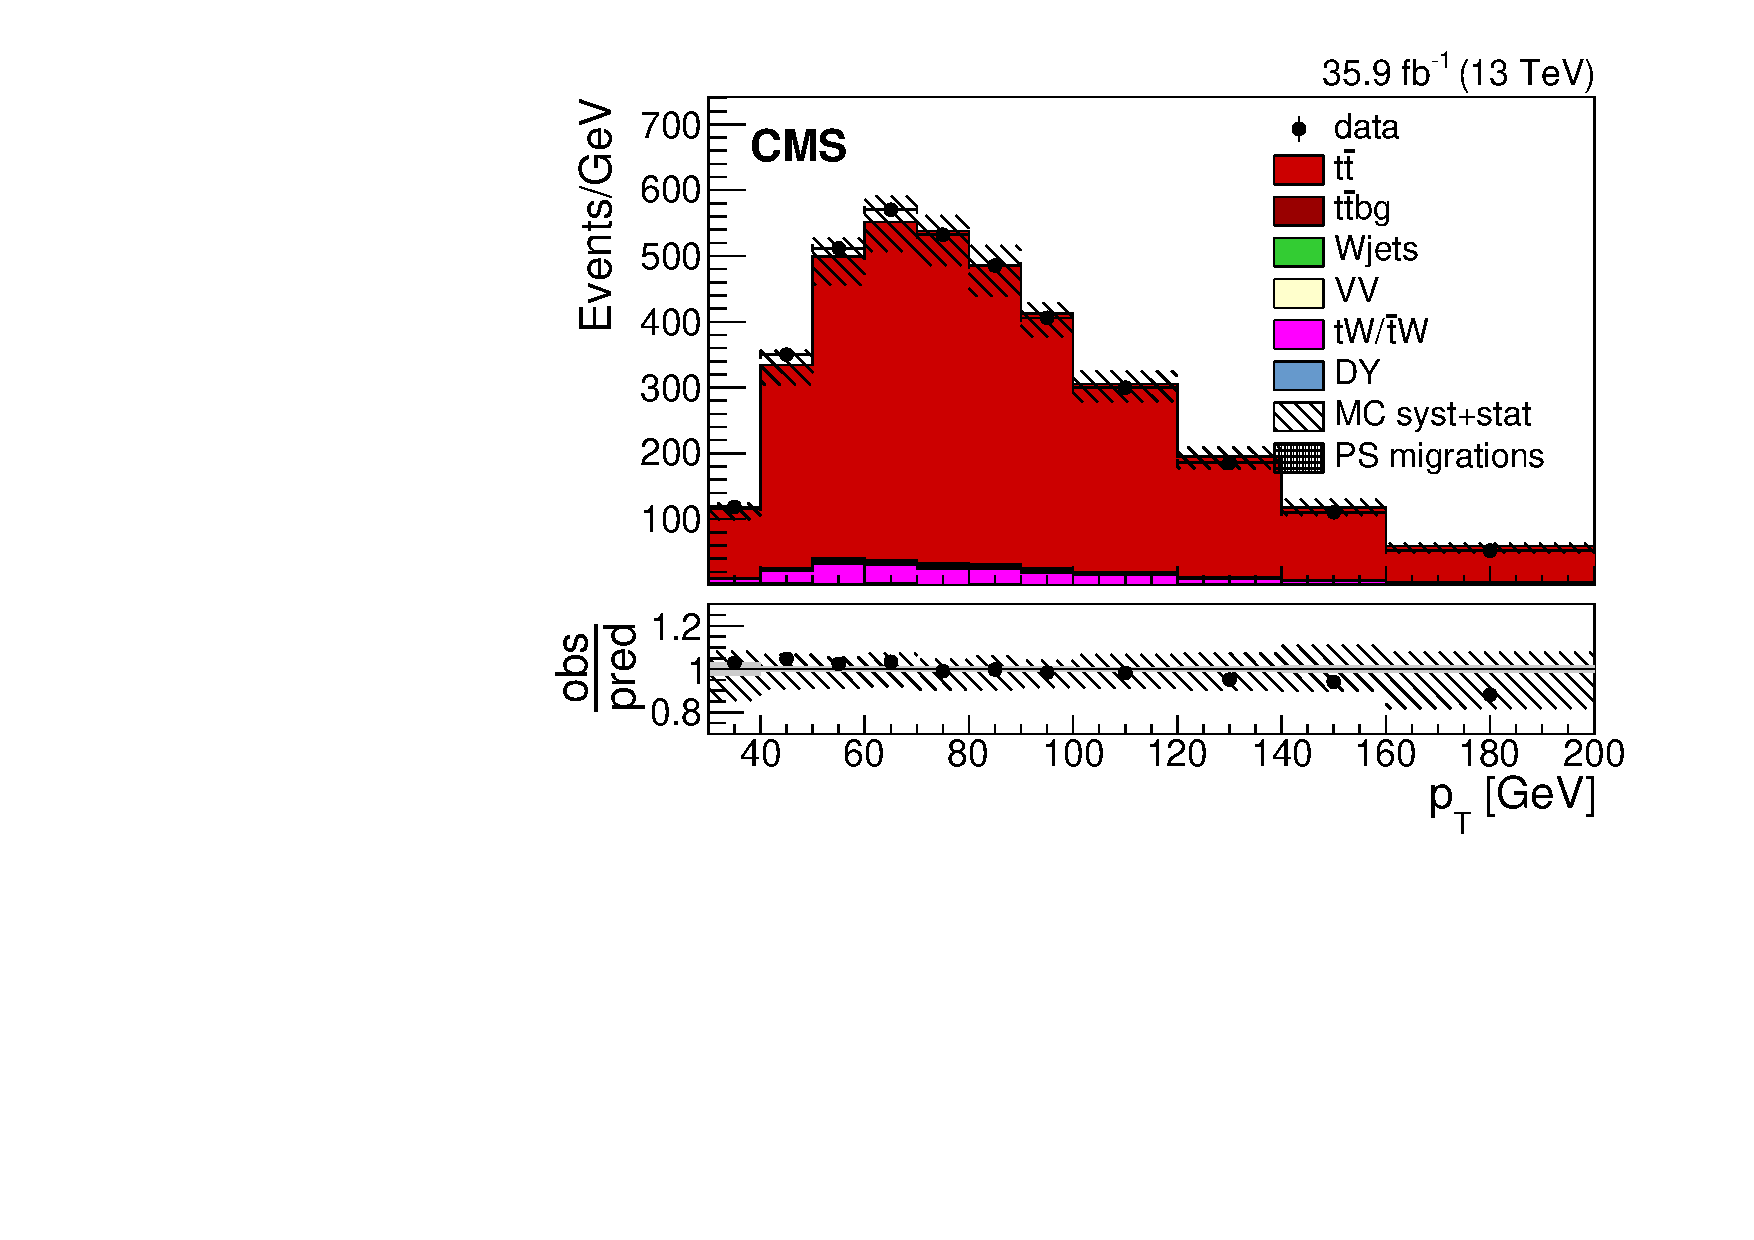
\includegraphics{CrossSection/Figures/ControlPlots/emu_sysnom/lead_jet_pt_1_1_b-jets_step_8.pdf}}
    \resizebox{0.32 \textwidth}{!}{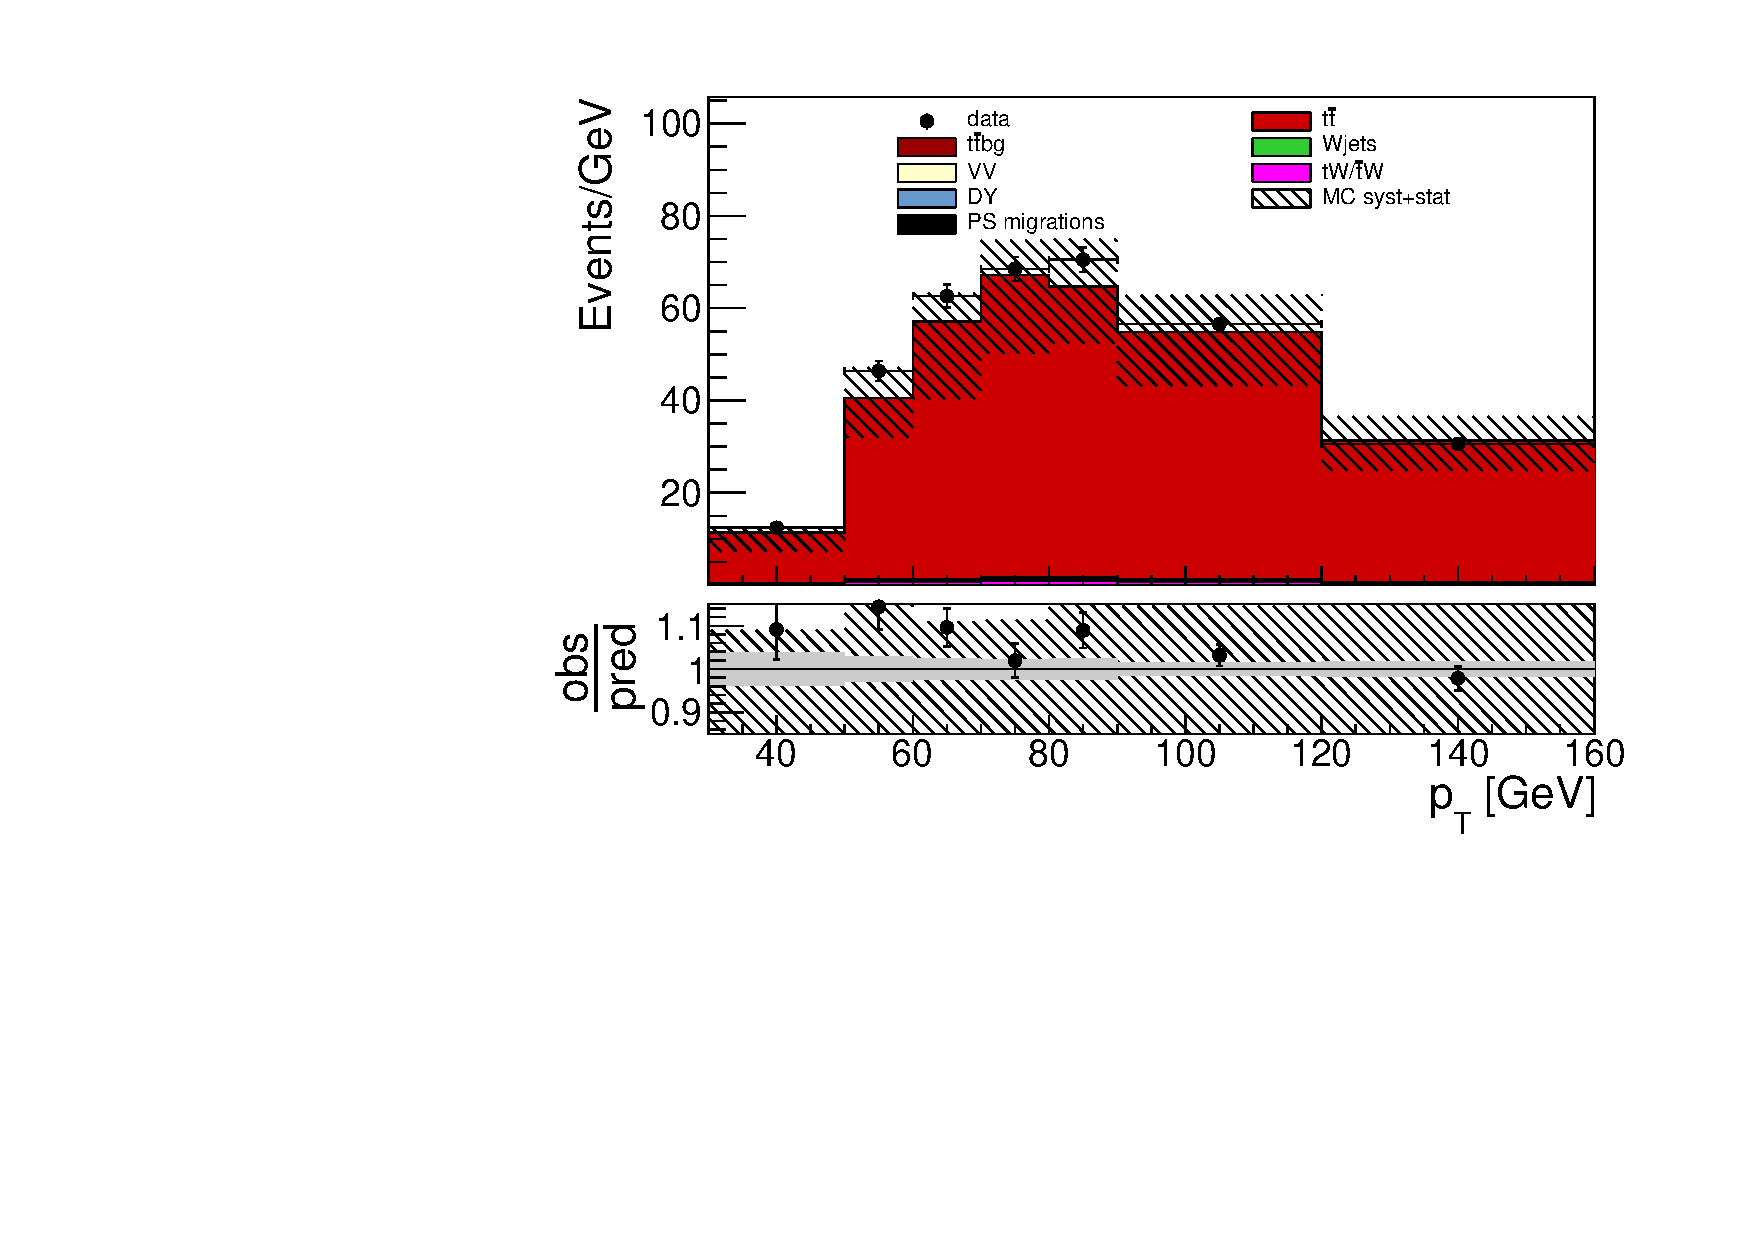
\includegraphics{CrossSection/Figures/ControlPlots/emu_sysnom/lead_jet_pt_2_1_b-jets_step_8.pdf}}
        
    \resizebox{0.32 \textwidth}{!}{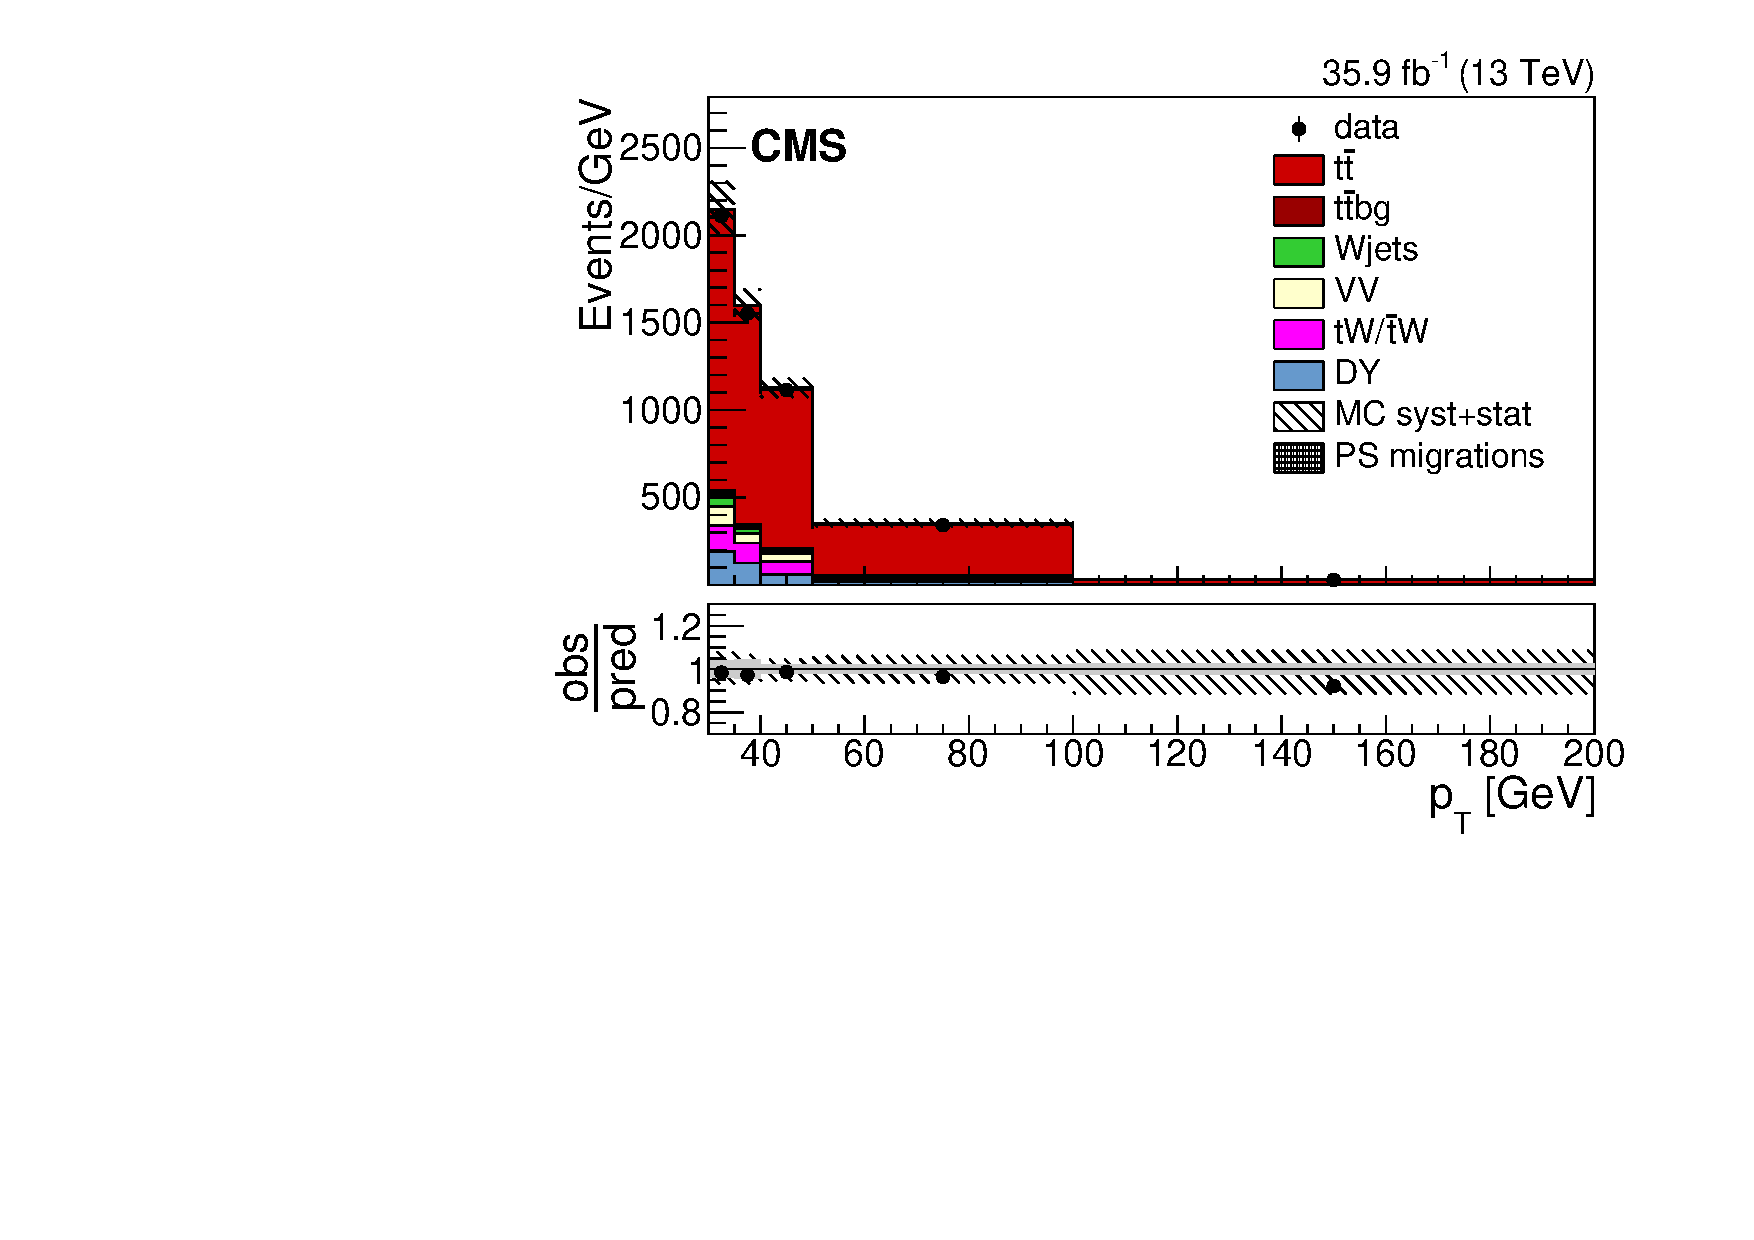
\includegraphics{CrossSection/Figures/ControlPlots/emu_sysnom/second_jet_pt_0_2_b-jets_step_8.pdf}}
    \resizebox{0.32 \textwidth}{!}{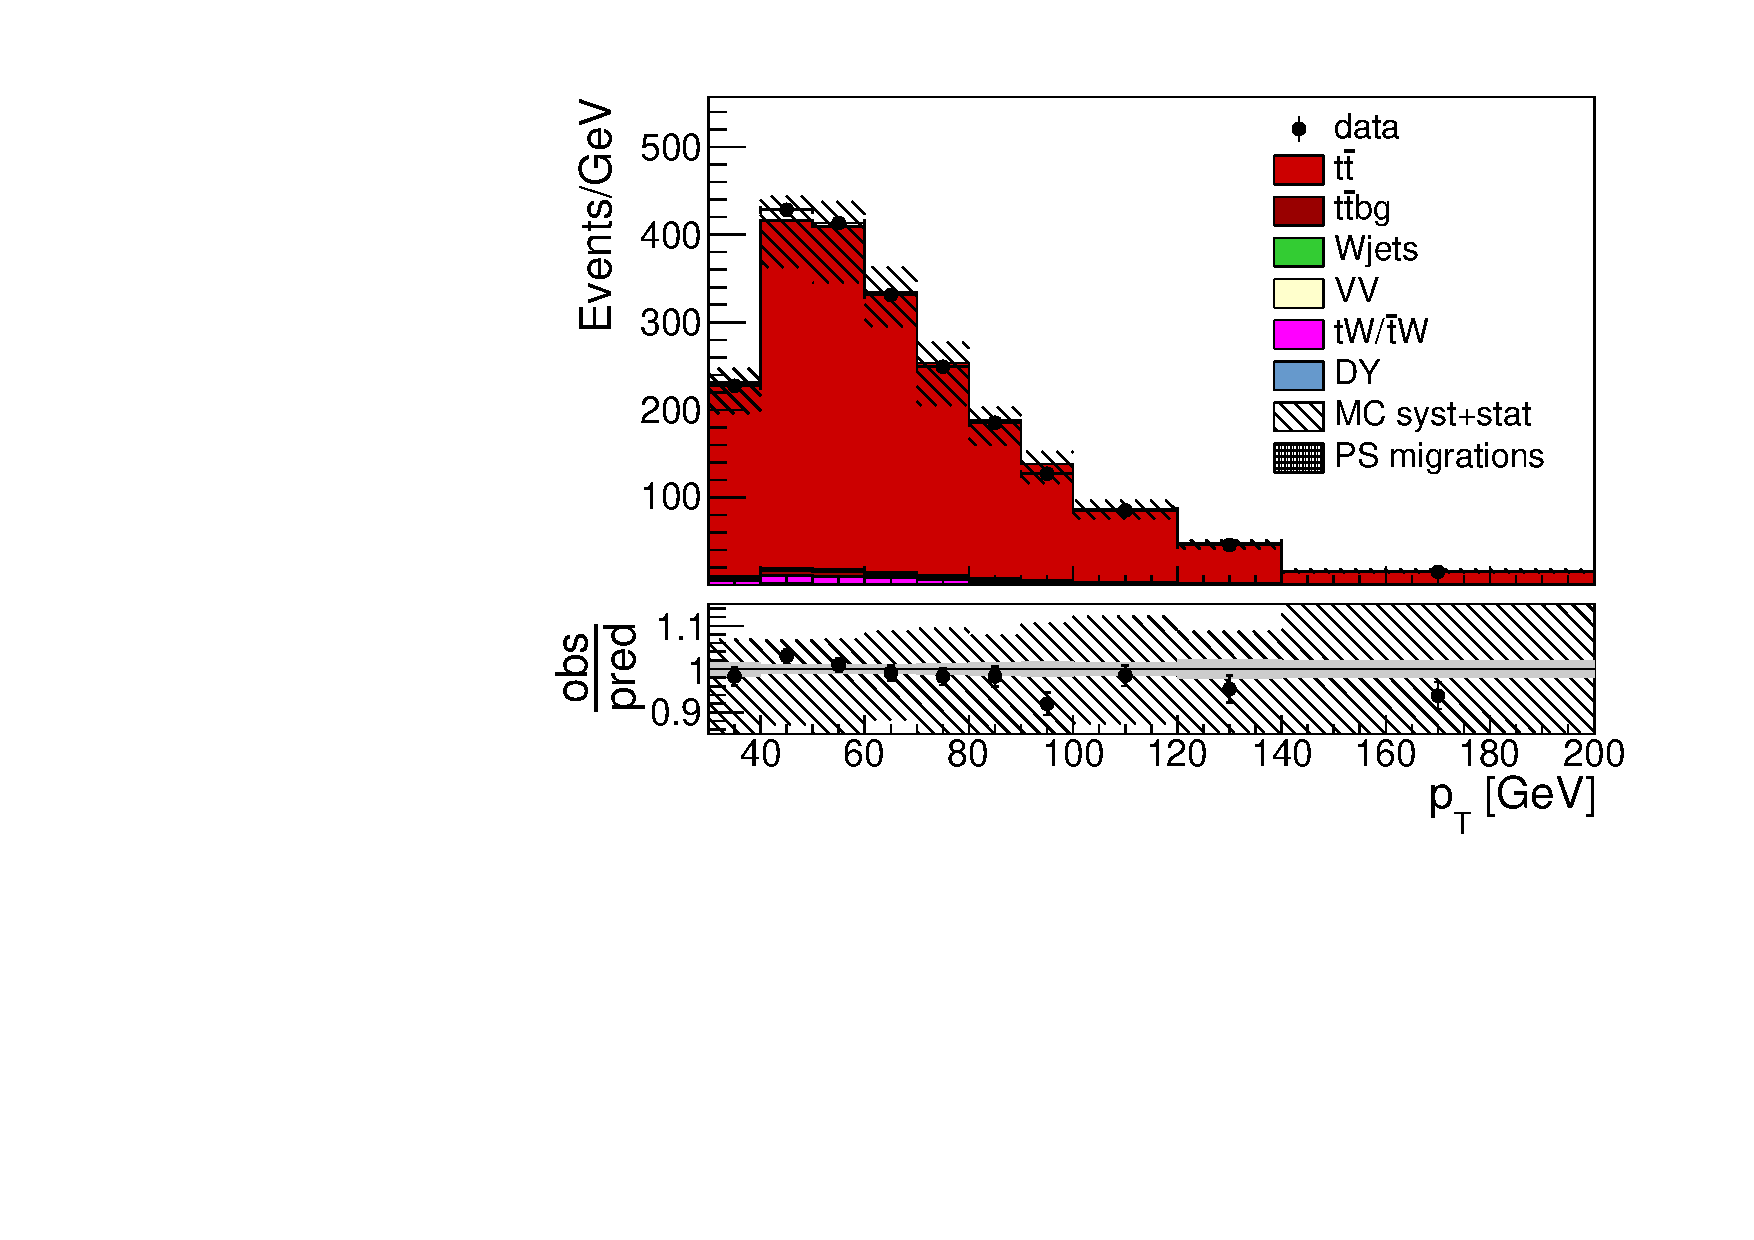
\includegraphics{CrossSection/Figures/ControlPlots/emu_sysnom/second_jet_pt_1_2_b-jets_step_8.pdf}}
    \resizebox{0.32 \textwidth}{!}{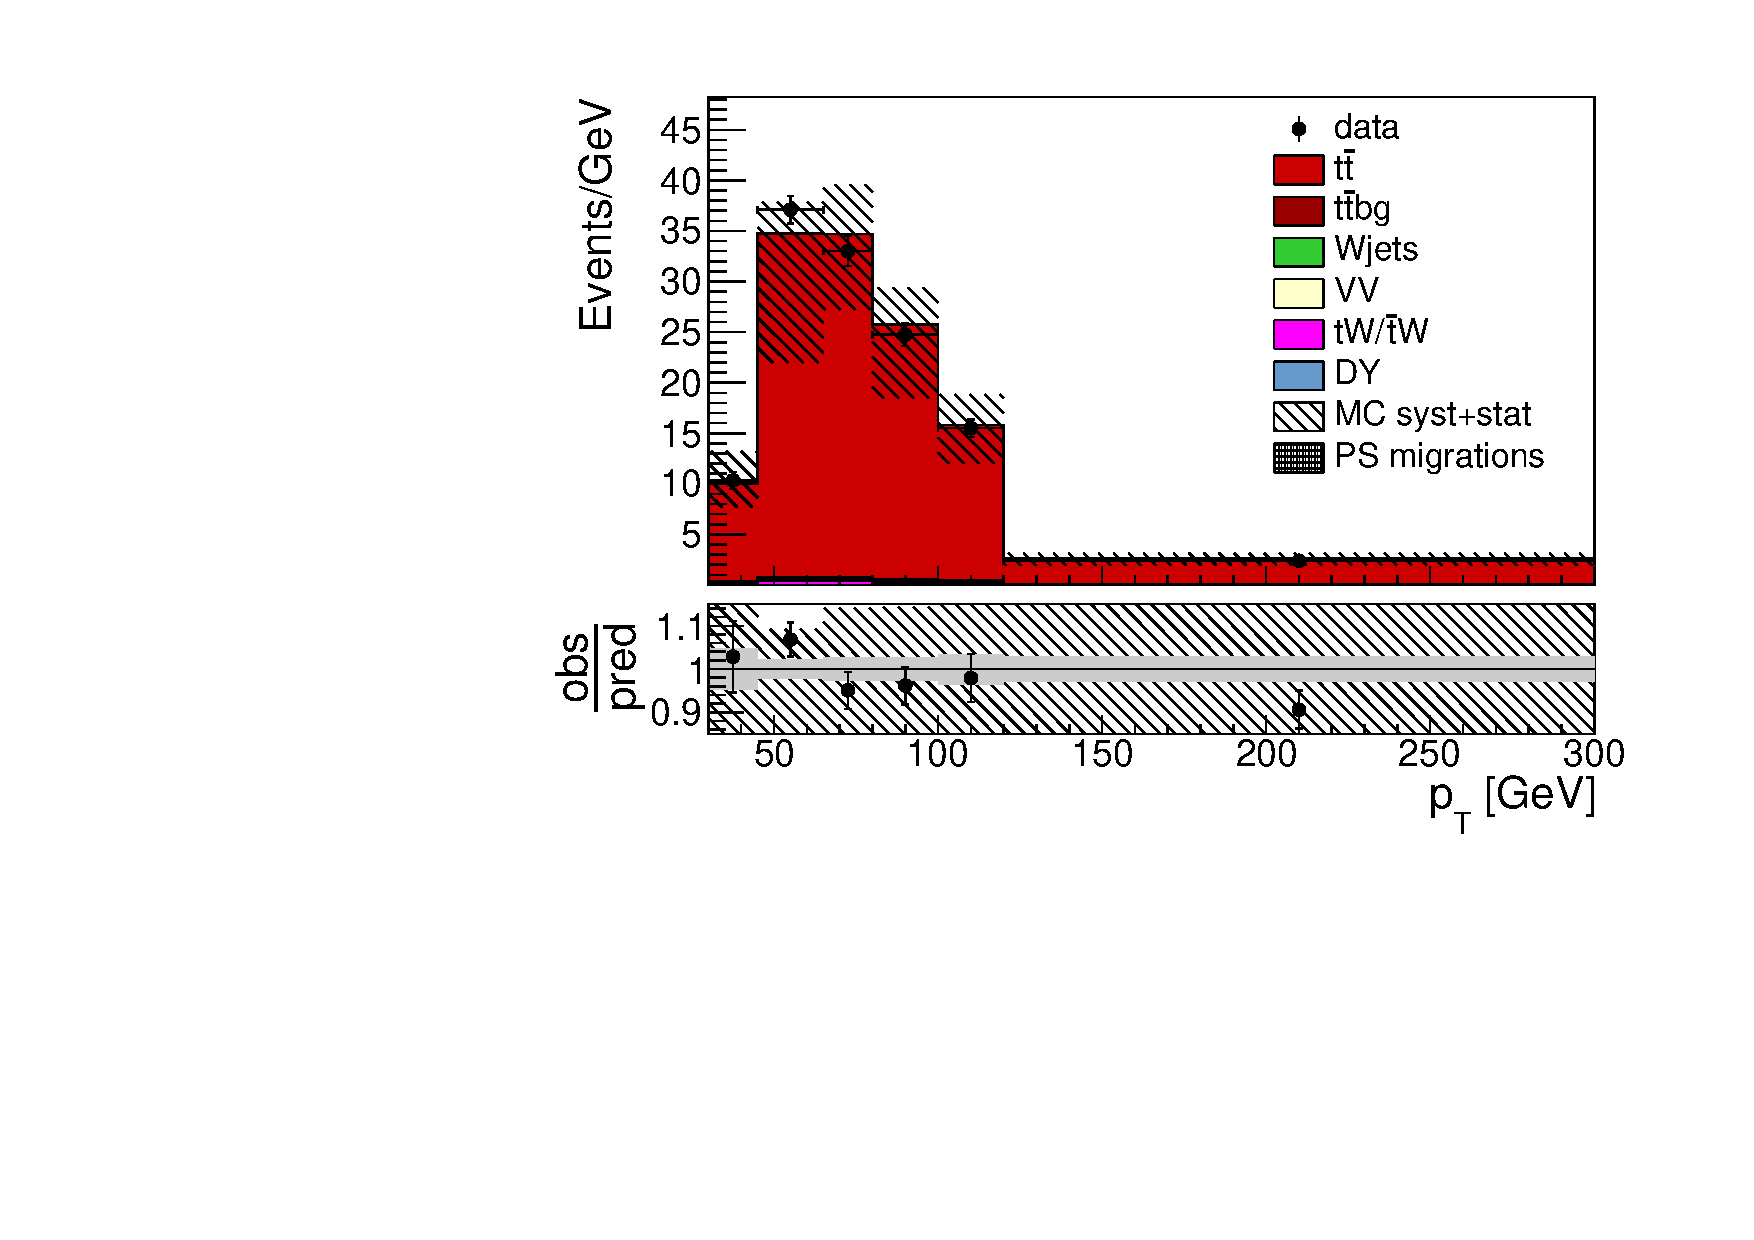
\includegraphics{CrossSection/Figures/ControlPlots/emu_sysnom/second_jet_pt_2_2_b-jets_step_8.pdf}}

    \resizebox{0.32 \textwidth}{!}{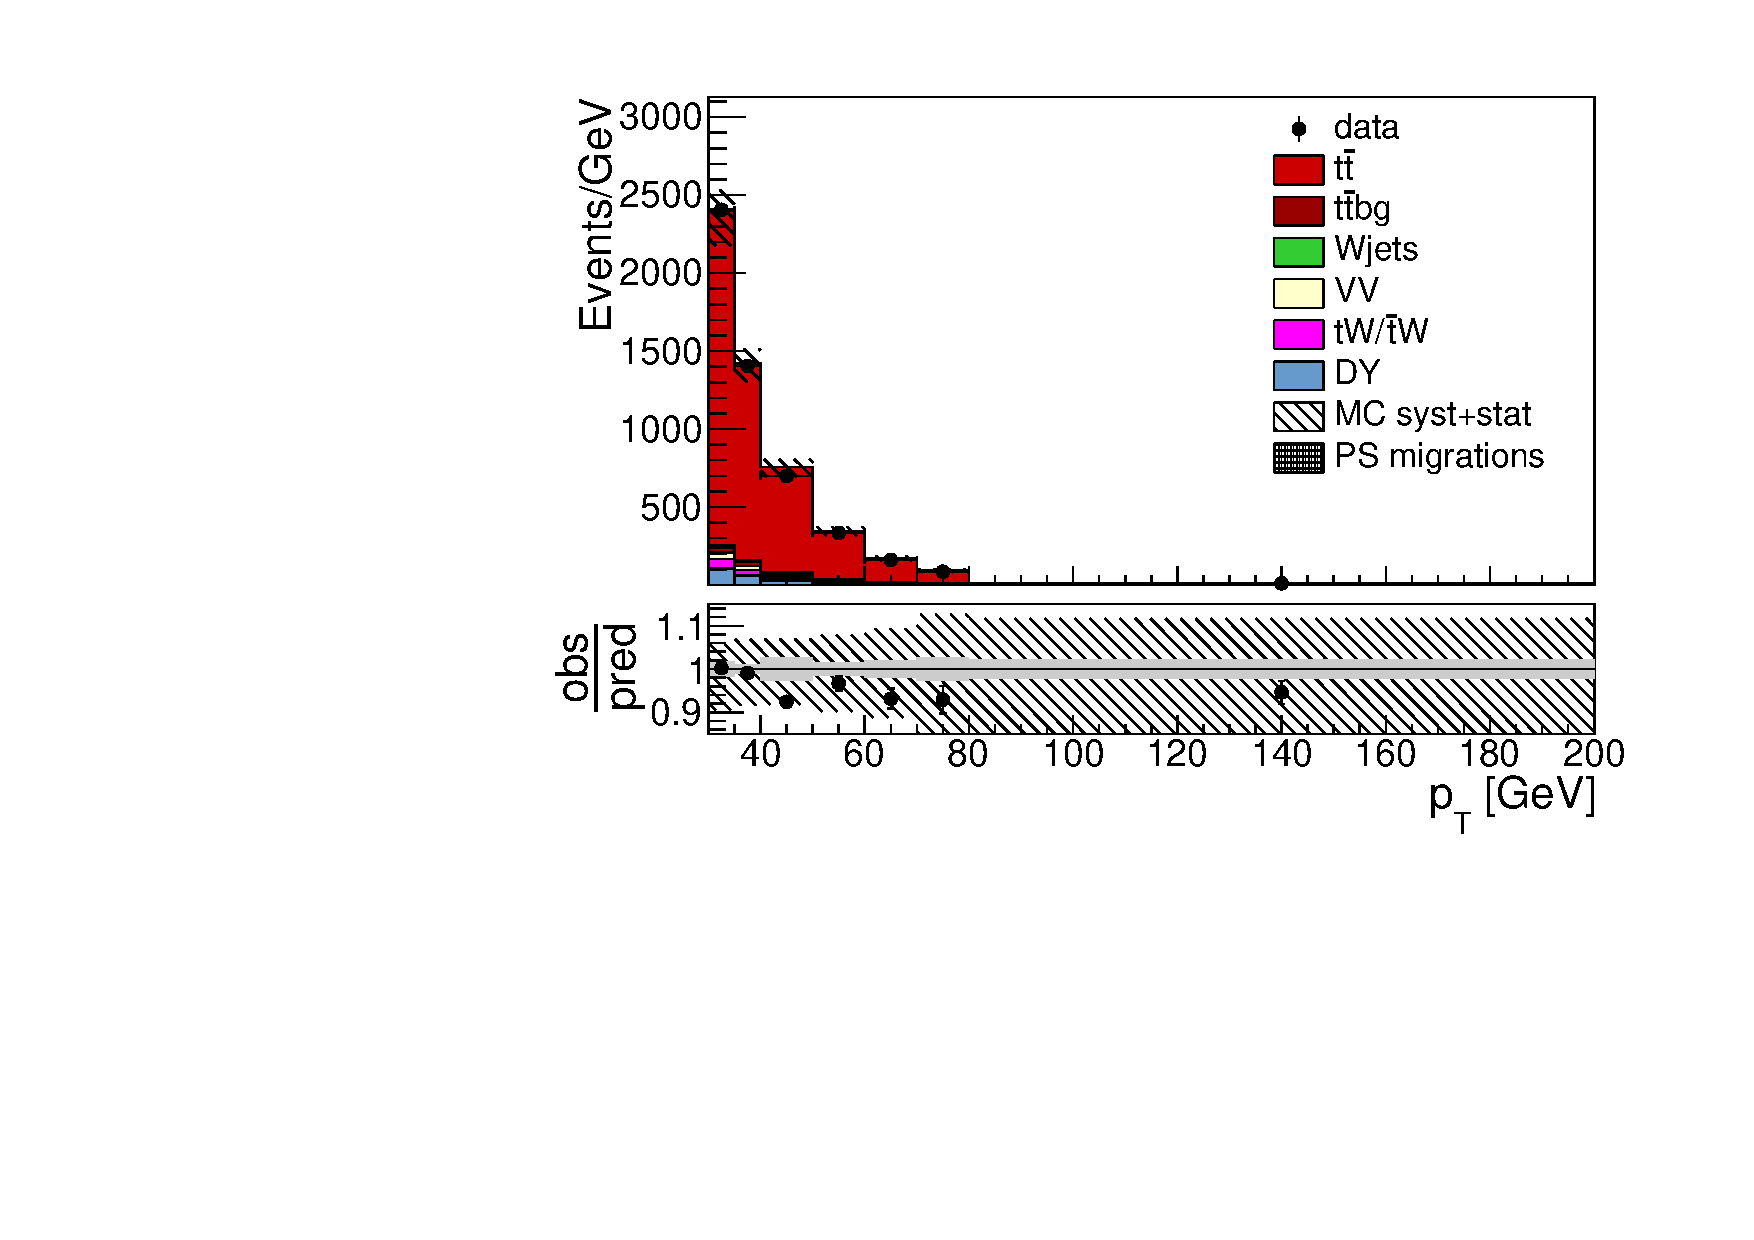
\includegraphics{CrossSection/Figures/ControlPlots/emu_sysnom/third_jet_pt_0_3_b-jets_step_8.pdf}}
    \resizebox{0.32 \textwidth}{!}{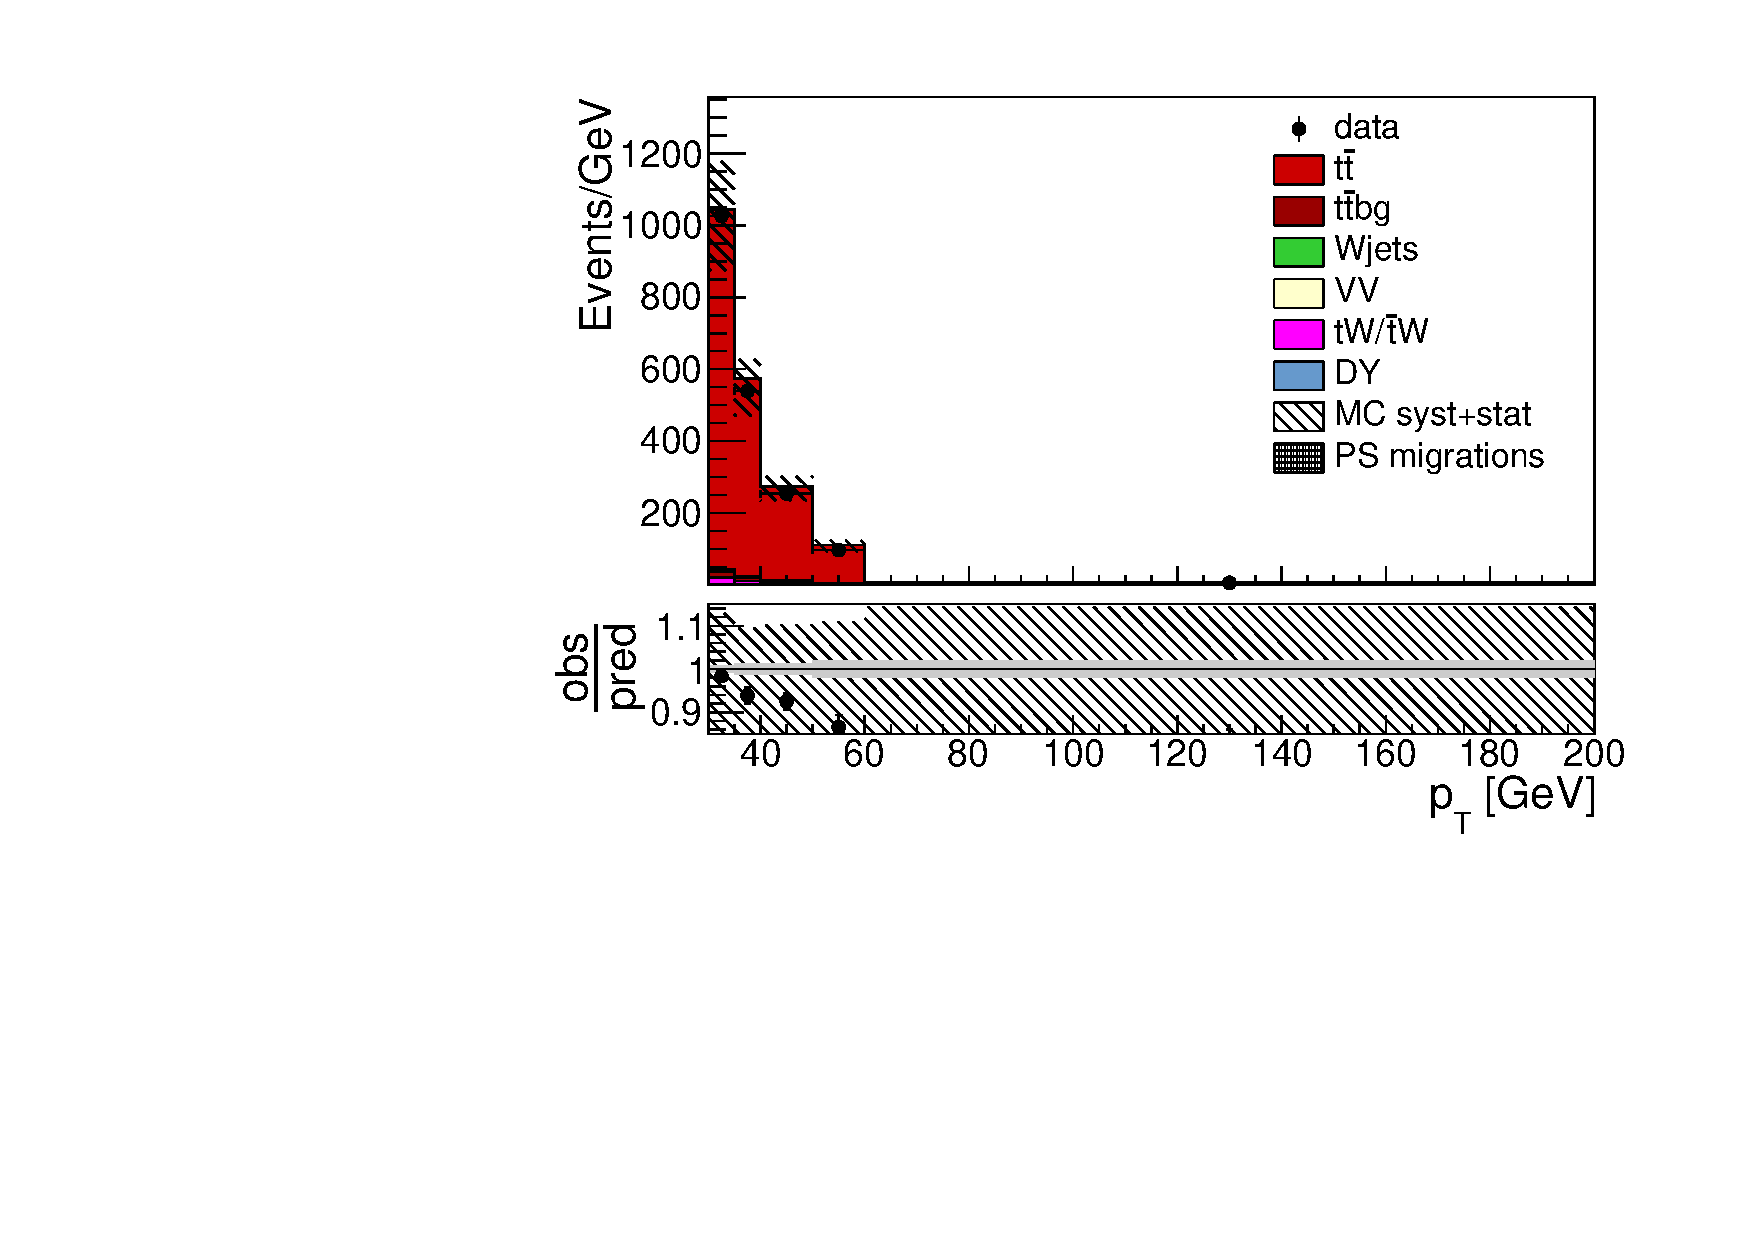
\includegraphics{CrossSection/Figures/ControlPlots/emu_sysnom/third_jet_pt_1_3_b-jets_step_8.pdf}}
    \resizebox{0.32 \textwidth}{!}{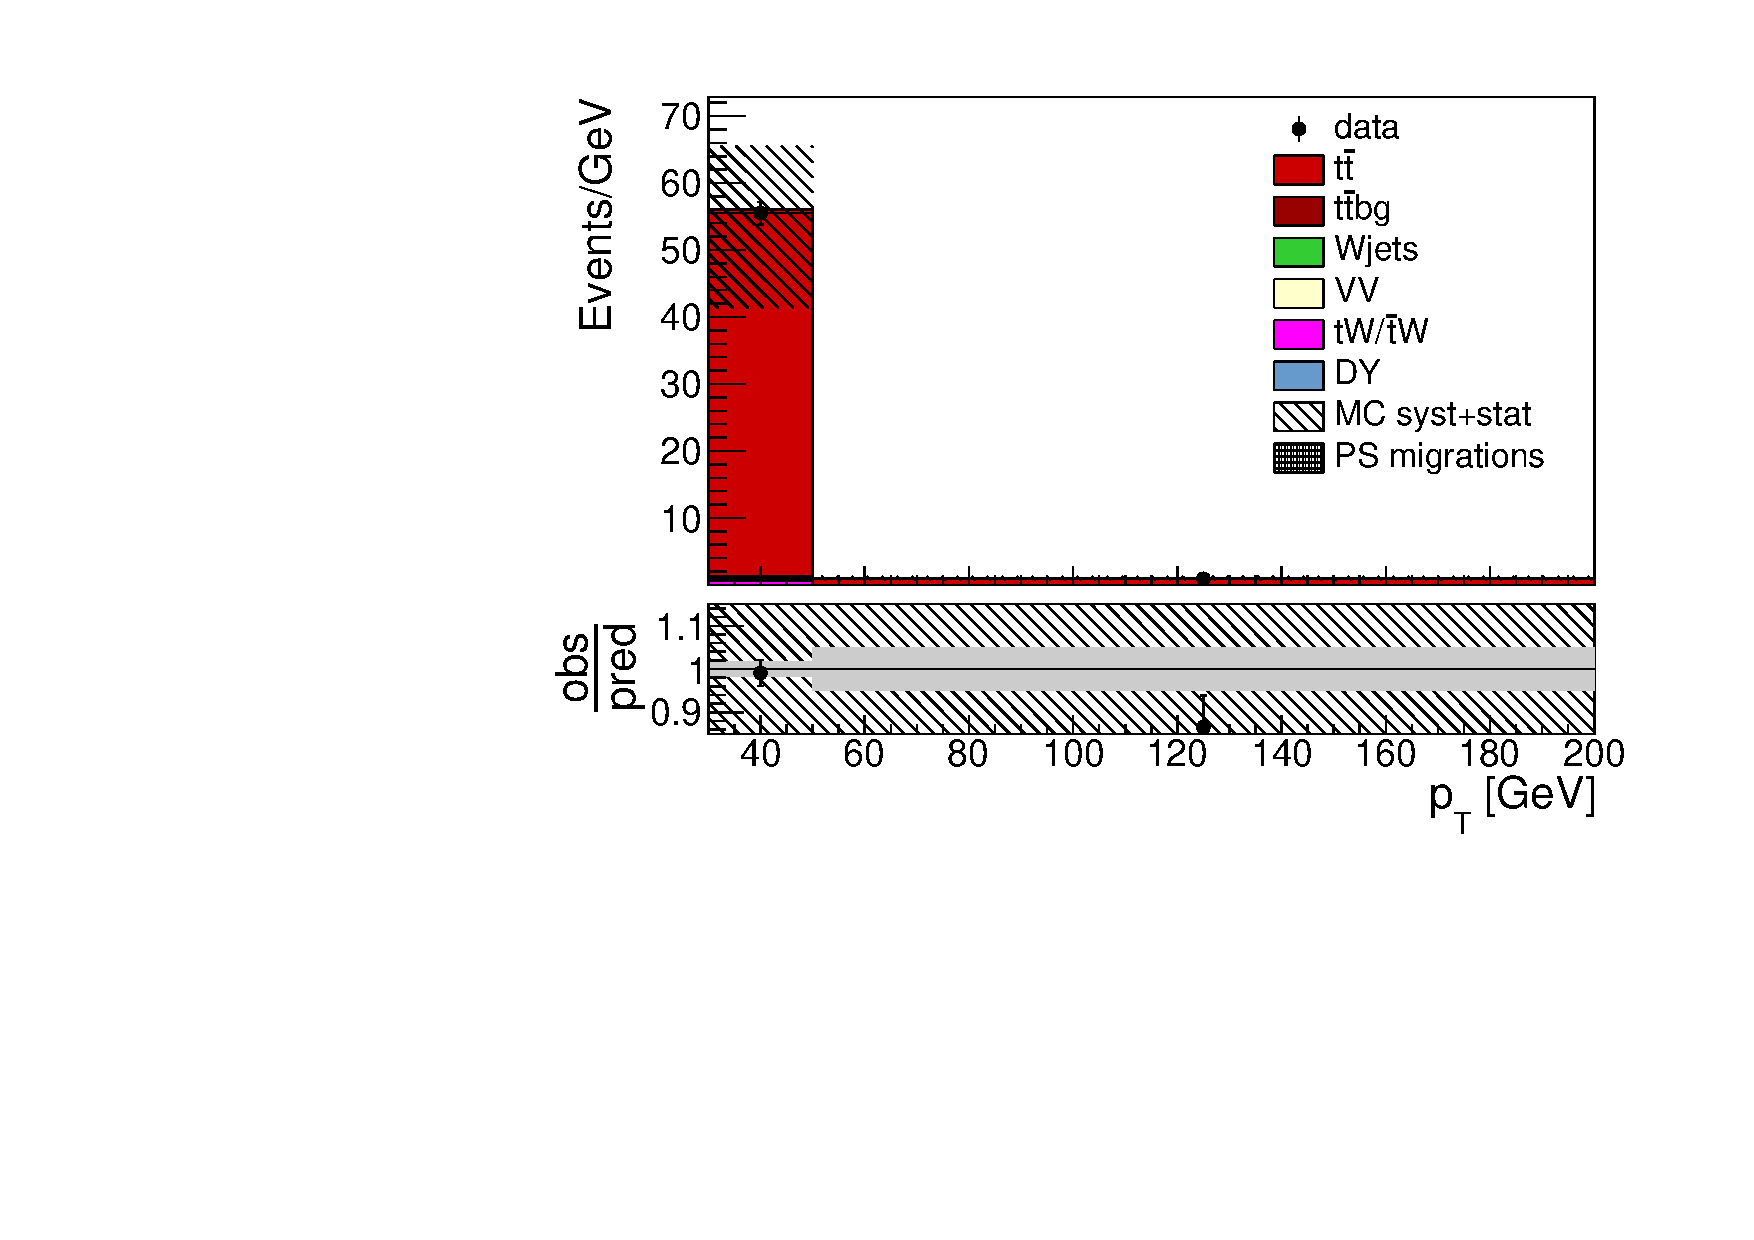
\includegraphics{CrossSection/Figures/ControlPlots/emu_sysnom/third_jet_pt_2_3_b-jets_step_8.pdf}}  

\caption{Pre-fit distributions (\emu channel) for events with zero as well as three or
  more b-tagged jets (left column): Total event yield for zero (top) and the trailing jet pt for one (second from top),
  two (second from bottom) or three or more (bottom) additional jets. The same for events with one
  b-tagged jet (middle column) and two b-tagged jets (right column) are
  shown below.   
  The hatched bands correspond to the total uncertainty on the sum of
  the predicted yields. The ratios of data to the sum of the
  predicted yields are shown at the bottom of each plot. Here, the solid
  gray band represents the contribution of the statistical uncertainty.  
       \label{fig:xsec_emu_inputdistr}}
  \end{center}
\end{figure}

\begin{figure}[htbp!]
  \begin{center}
    \resizebox{0.240 \textwidth}{!}{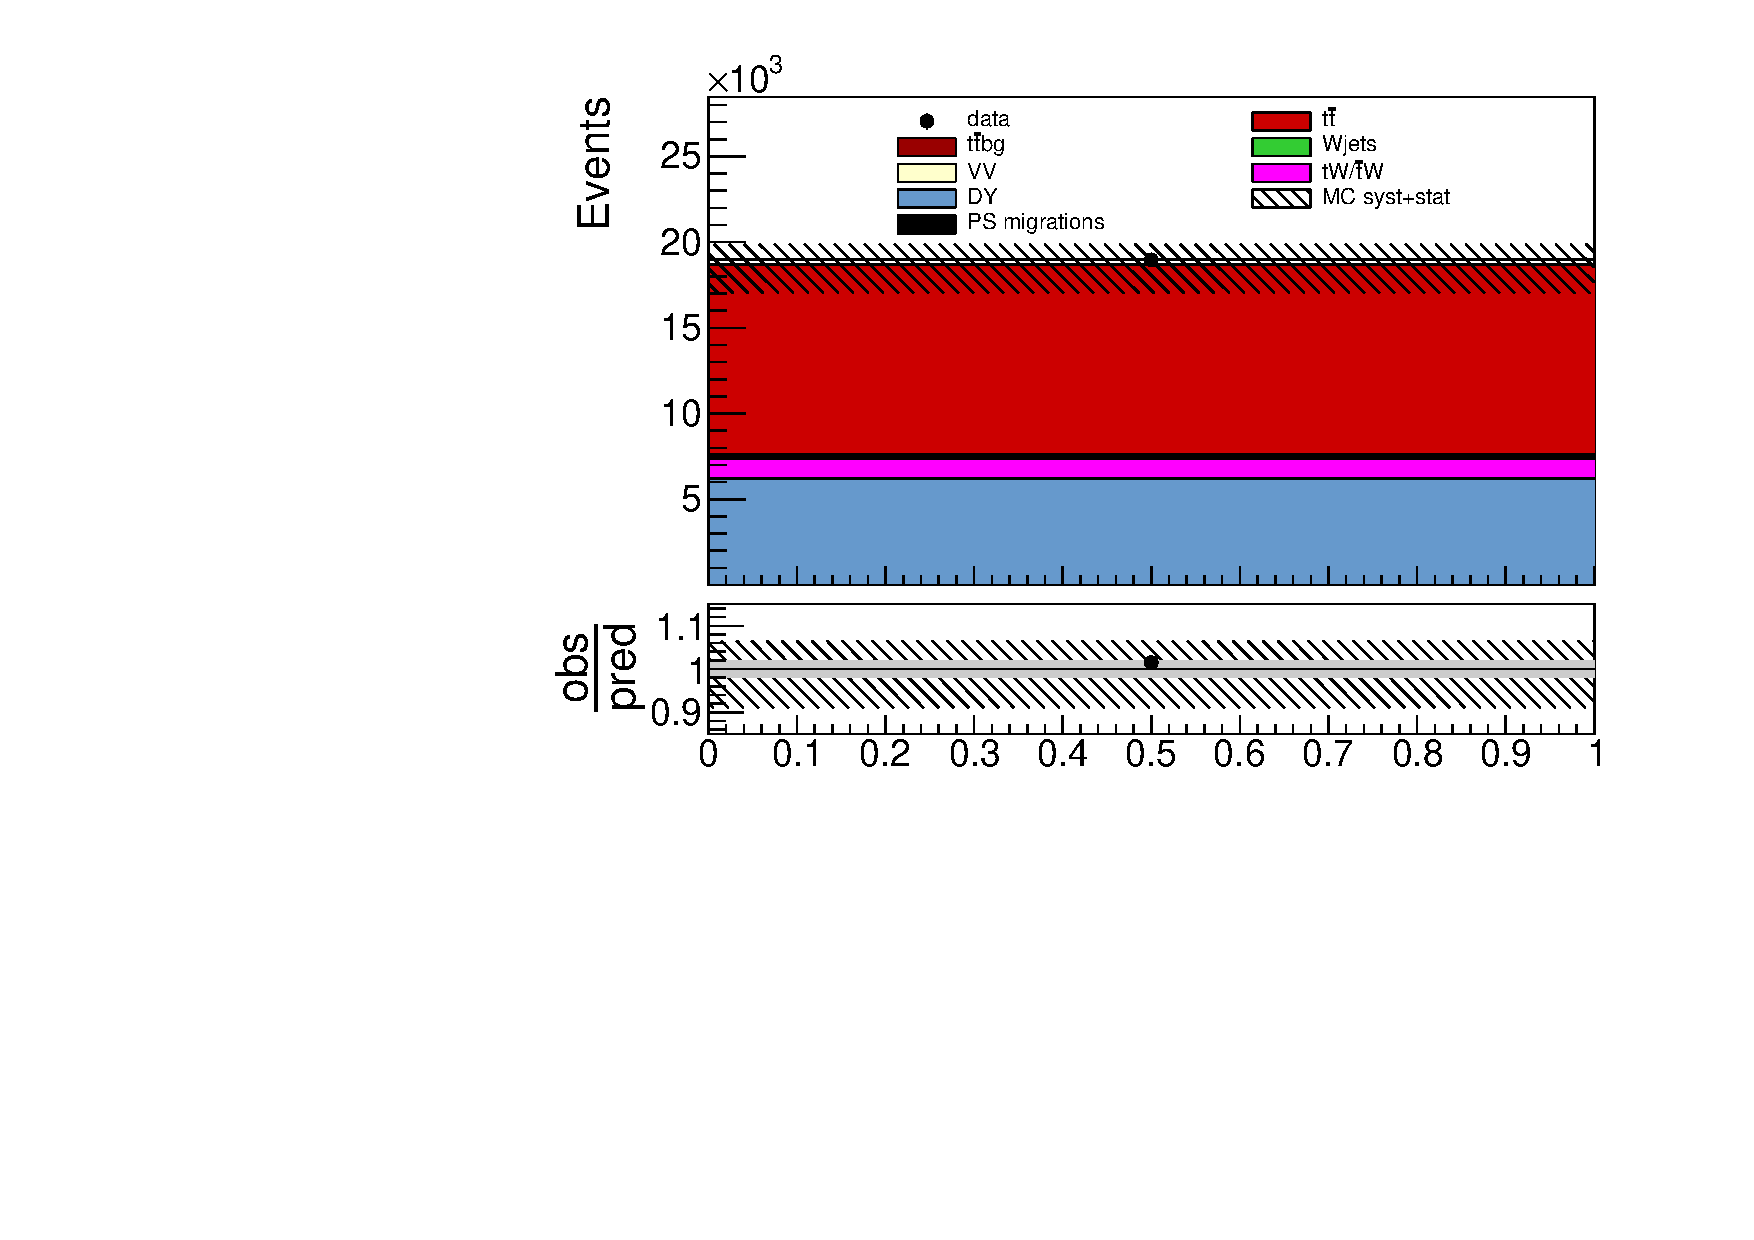
\includegraphics{CrossSection/Figures/ControlPlots/mumu_sysnom/total_1_0_b-jets_step_8.pdf}}
    \resizebox{0.240 \textwidth}{!}{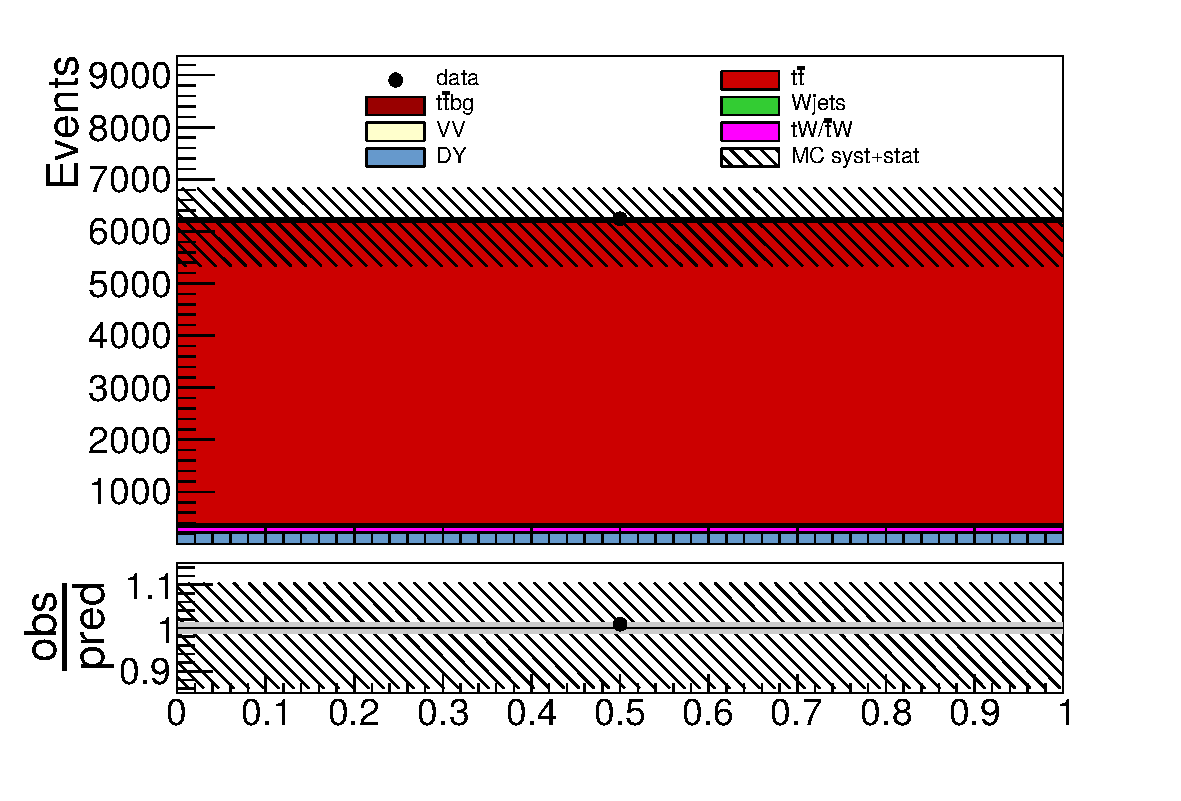
\includegraphics{CrossSection/Figures/ControlPlots/mumu_sysnom/total_2_0_b-jets_step_8.pdf}} \\

    \resizebox{0.40 \textwidth}{!}{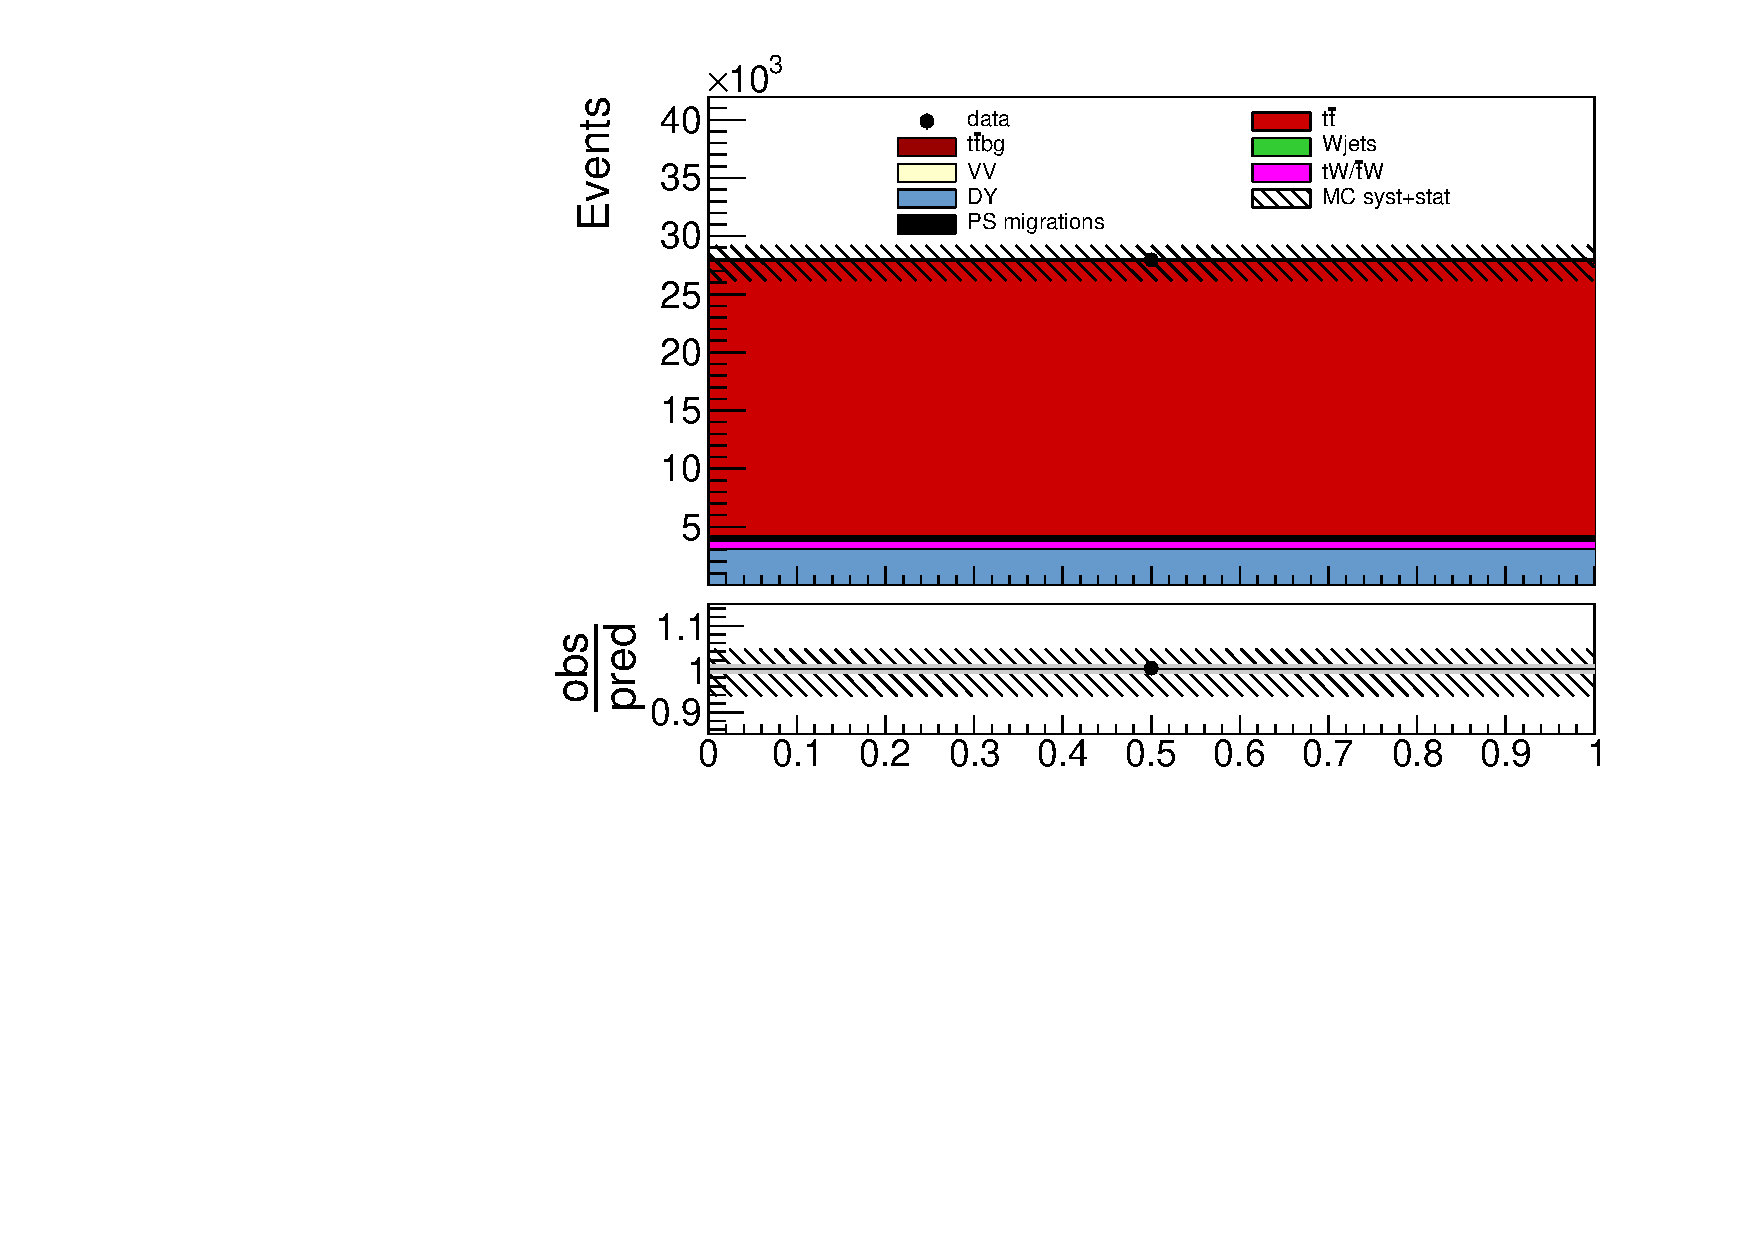
\includegraphics{CrossSection/Figures/ControlPlots/mumu_sysnom/total_1_1_b-jets_step_8.pdf}}
    \resizebox{0.40 \textwidth}{!}{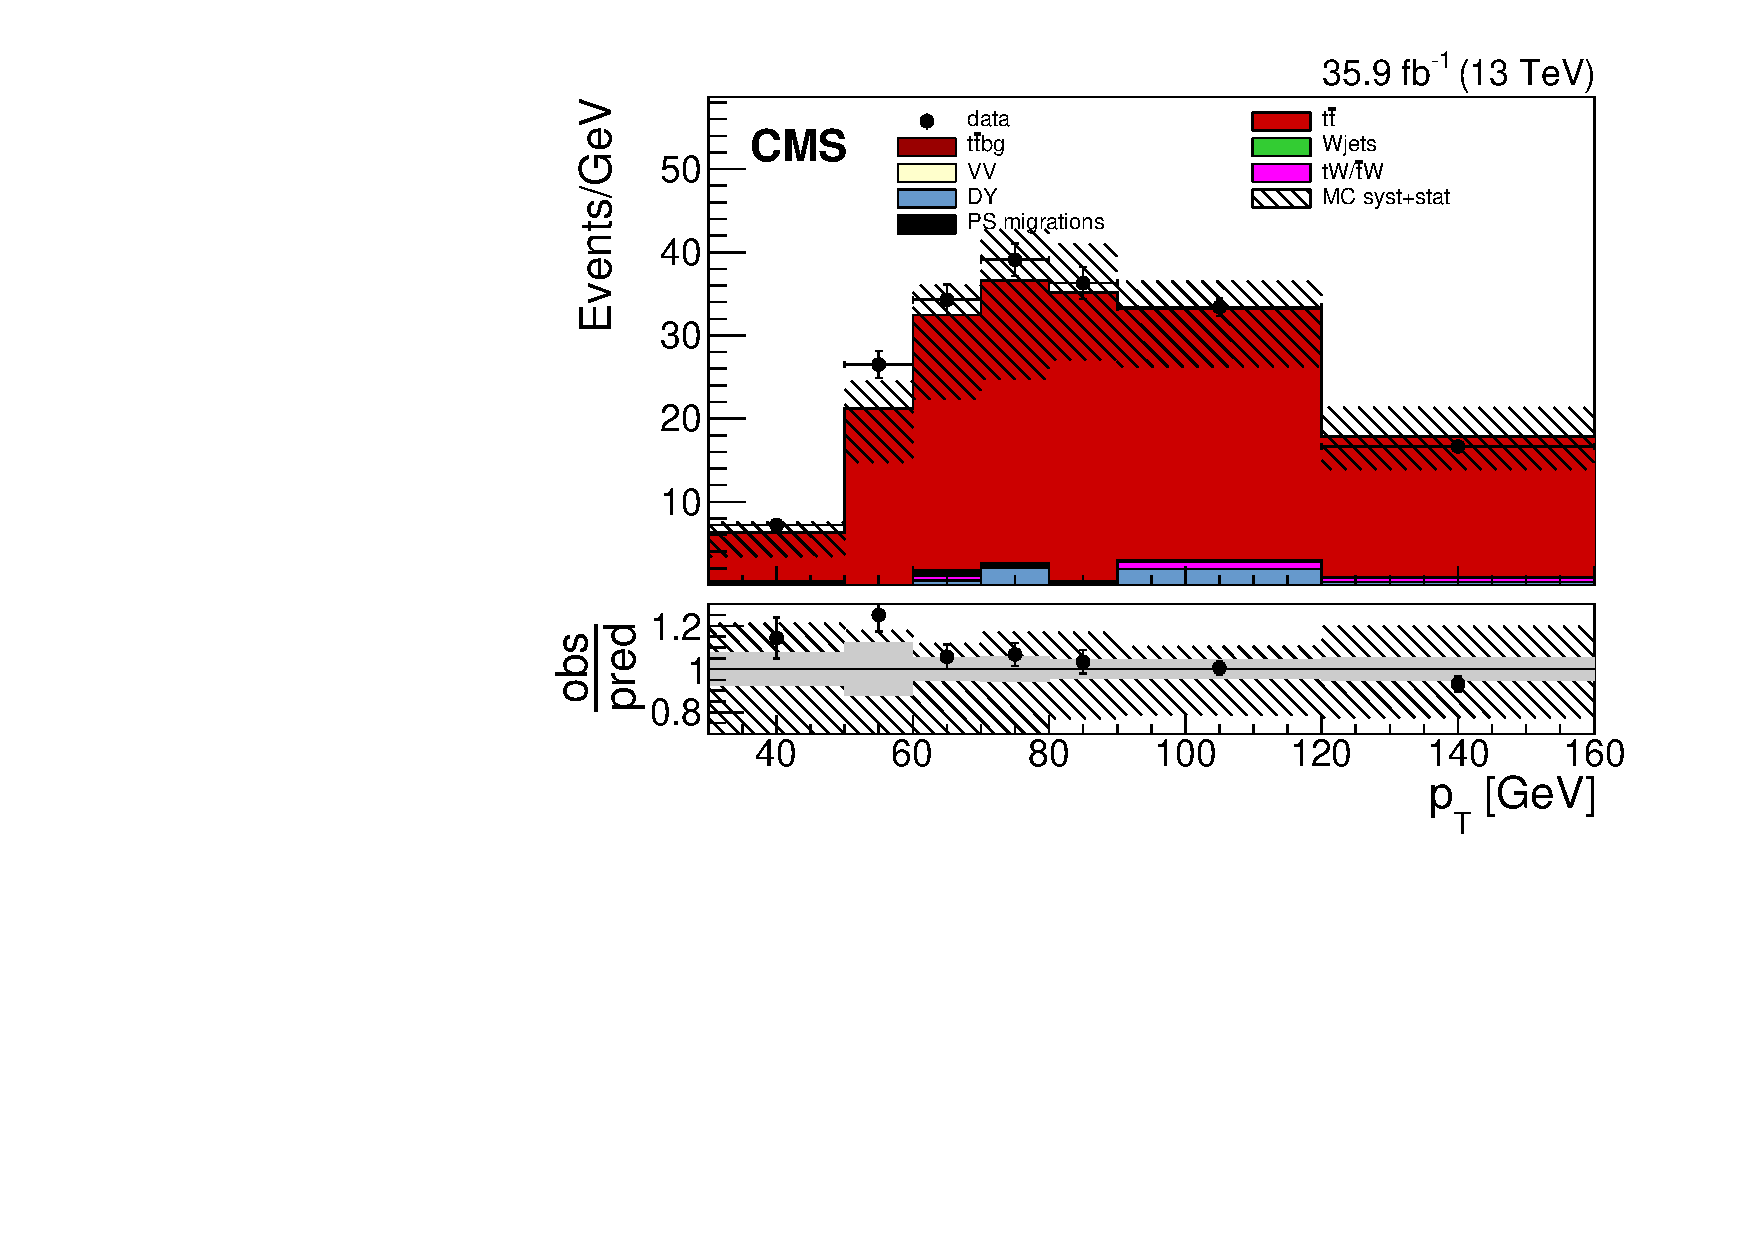
\includegraphics{CrossSection/Figures/ControlPlots/mumu_sysnom/lead_jet_pt_2_1_b-jets_step_8.pdf}}\\
        
    \resizebox{0.4 \textwidth}{!}{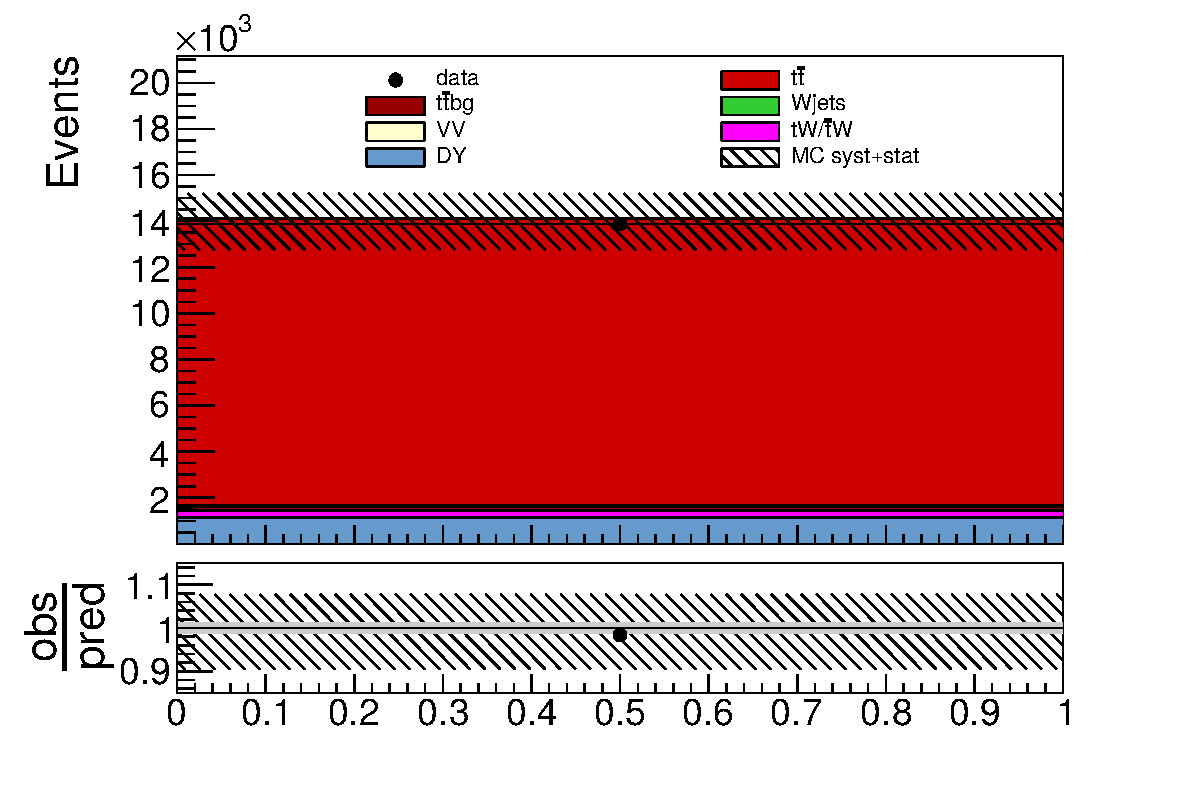
\includegraphics{CrossSection/Figures/ControlPlots/mumu_sysnom/total_1_2_b-jets_step_8.pdf}}
    \resizebox{0.4 \textwidth}{!}{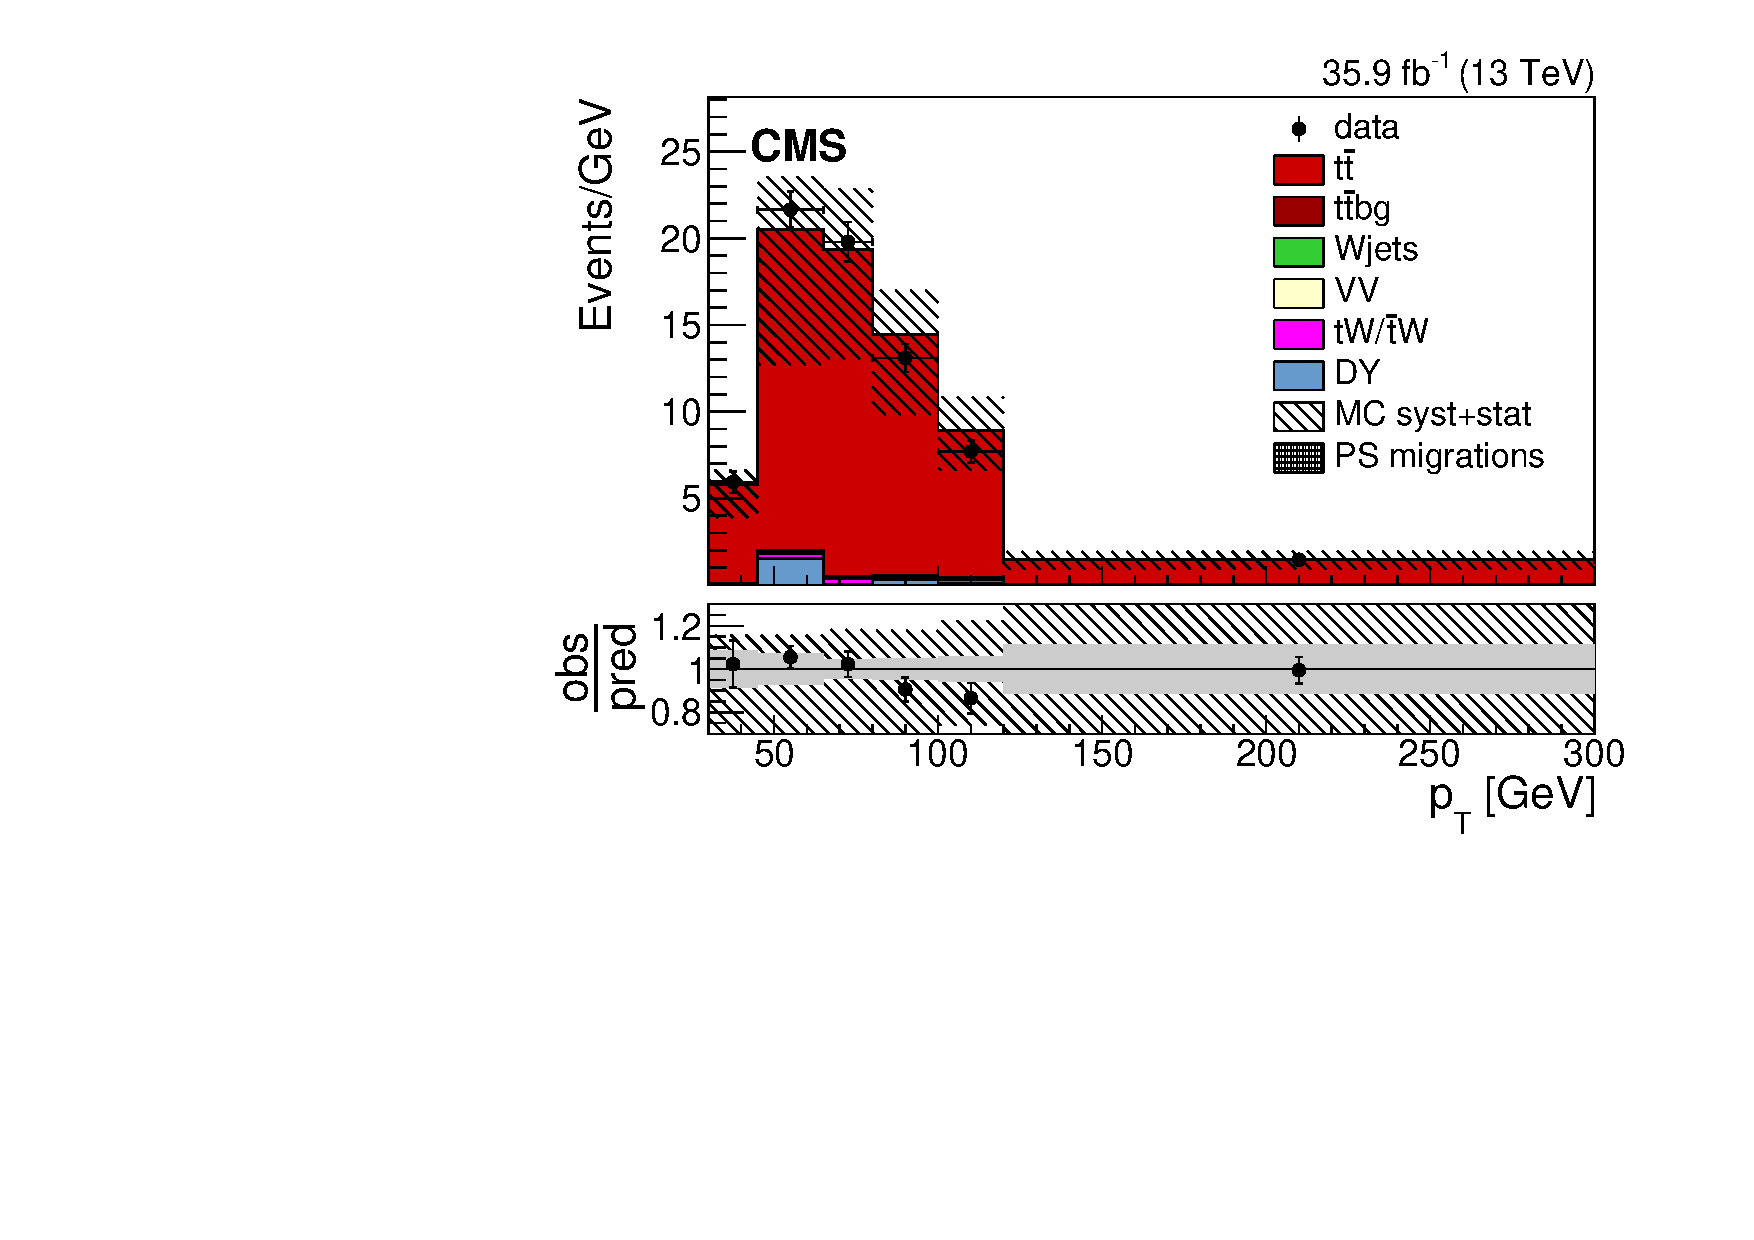
\includegraphics{CrossSection/Figures/ControlPlots/mumu_sysnom/second_jet_pt_2_2_b-jets_step_8.pdf}}\\

    \resizebox{0.4 \textwidth}{!}{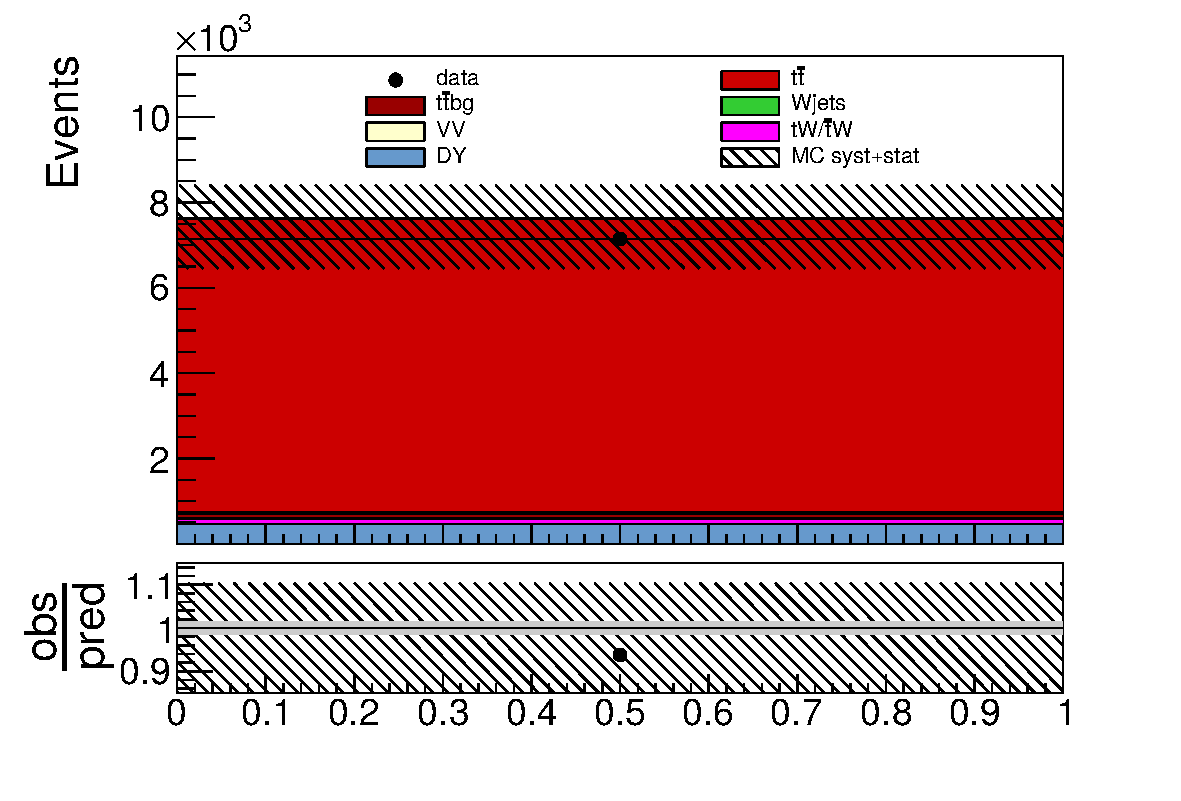
\includegraphics{CrossSection/Figures/ControlPlots/mumu_sysnom/total_1_3_b-jets_step_8.pdf}}
    \resizebox{0.4 \textwidth}{!}{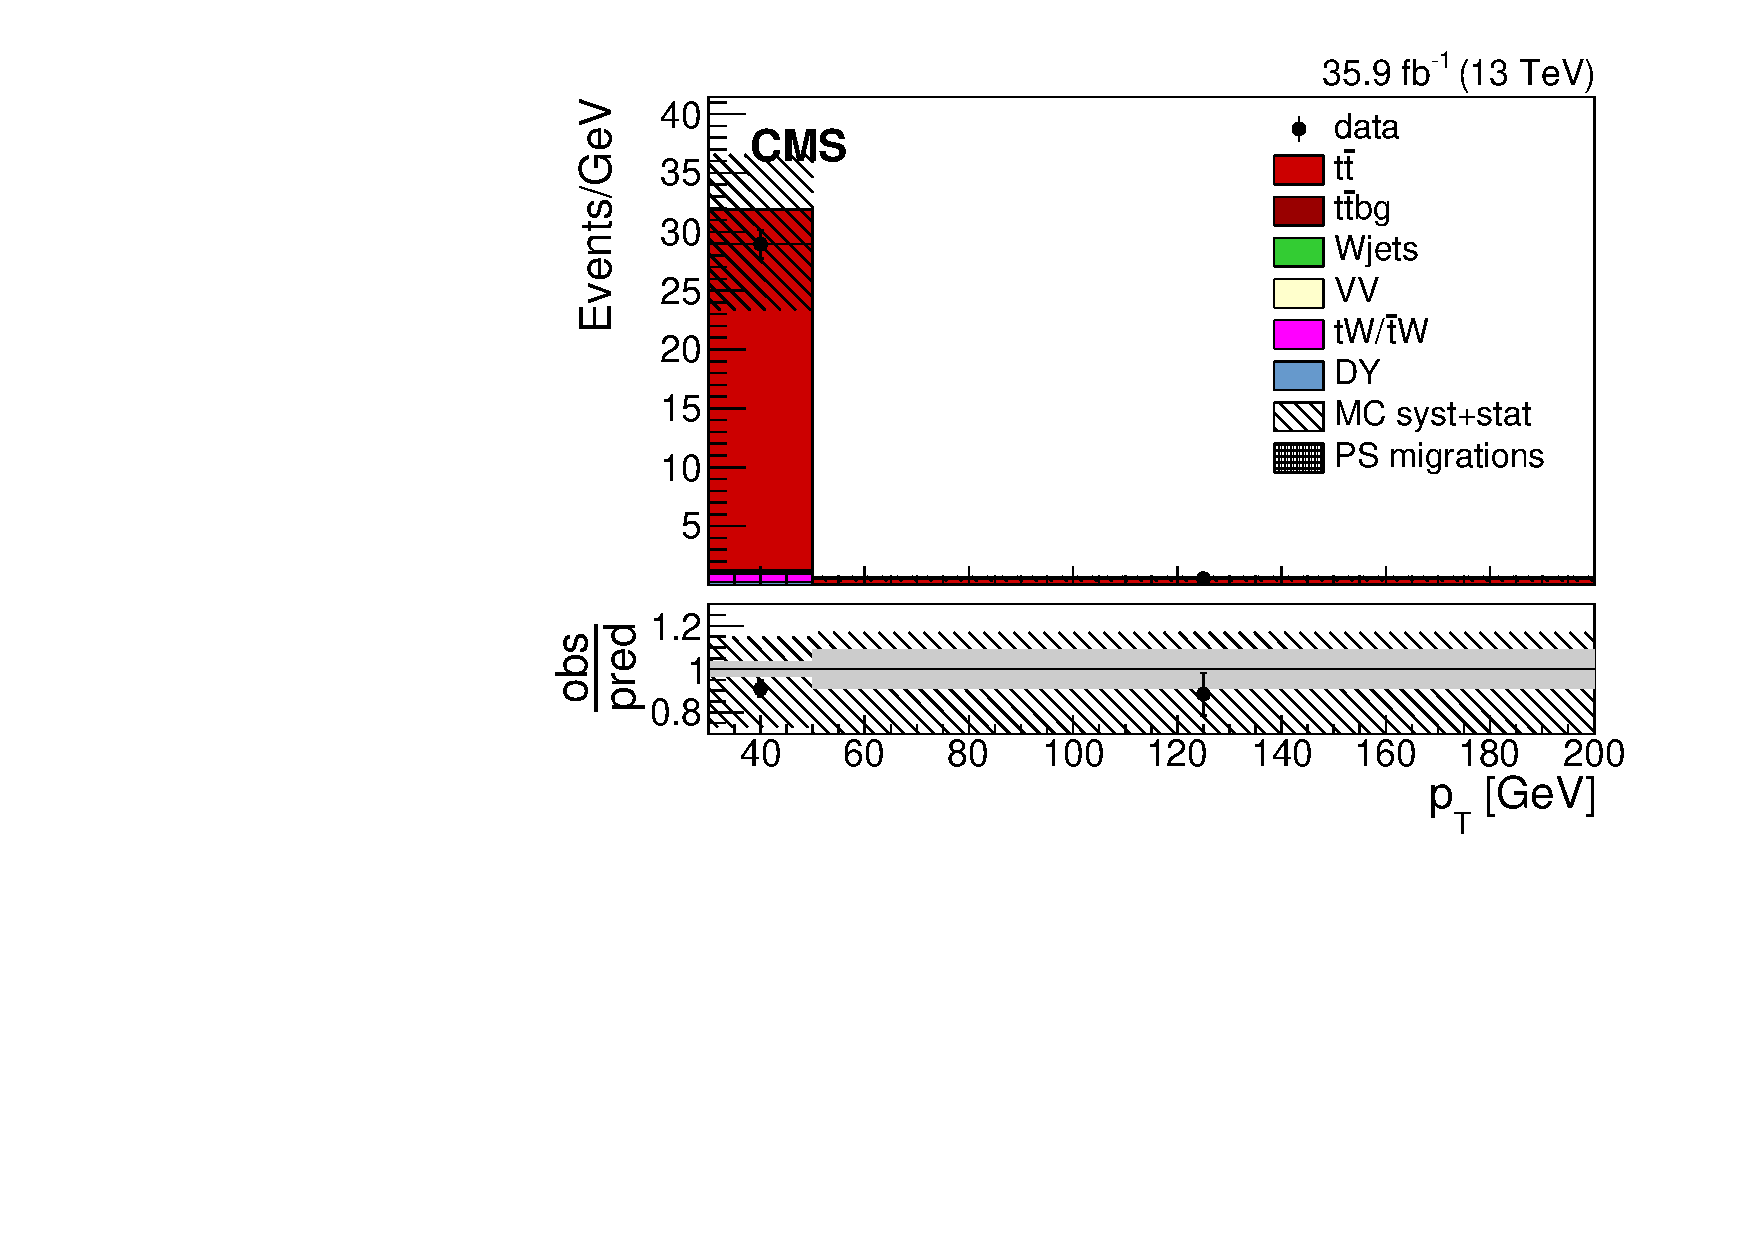
\includegraphics{CrossSection/Figures/ControlPlots/mumu_sysnom/third_jet_pt_2_3_b-jets_step_8.pdf}}  
\caption{Pre-fit distributions (\mumu channel): 
  The left column shows events with one b-tagged jet and the total event yield for events with zero (top), one (second from top)
  two (second from bottom) or three or more additional jets (bottom).
  The right column shows events with two b-tagged jets and the total yield for events with zero additional jets (top),
  the trailing jet pt for one (second from top),
  two (second from bottom) or three or more (bottom) additional jets.
  The hatched bands correspond to the total uncertainty on the sum of
  the predicted yields. The ratios of data to the sum of the
  predicted yields are shown at the bottom of each plot. Here, the solid
  gray band represents the contribution of the statistical uncertainty.  
       \label{fig:xsec_mumu_inputdistr}}
  \end{center}
\end{figure}

\begin{figure}[htbp!]
  \begin{center}
    \resizebox{0.24 \textwidth}{!}{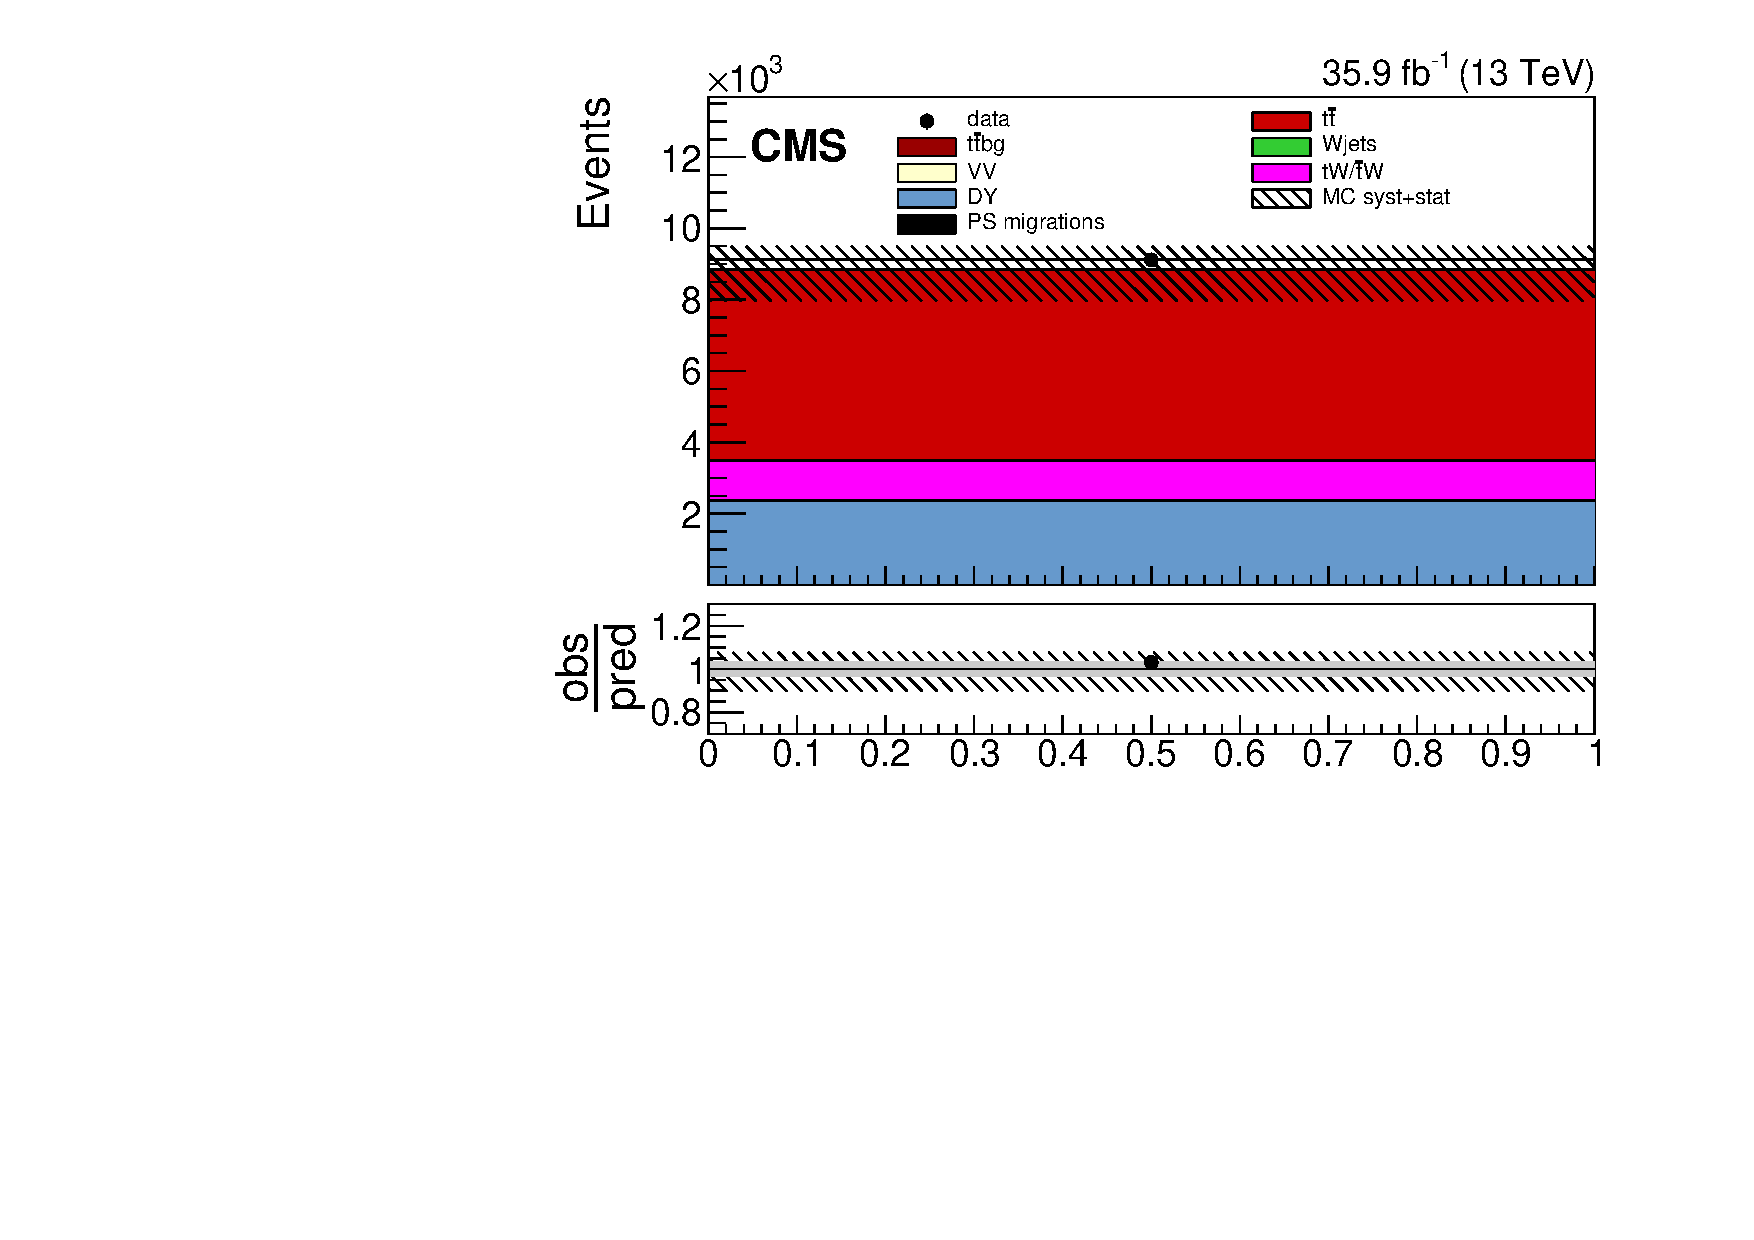
\includegraphics{CrossSection/Figures/ControlPlots/ee_sysnom/total_1_0_b-jets_step_8.pdf}}
    \resizebox{0.24 \textwidth}{!}{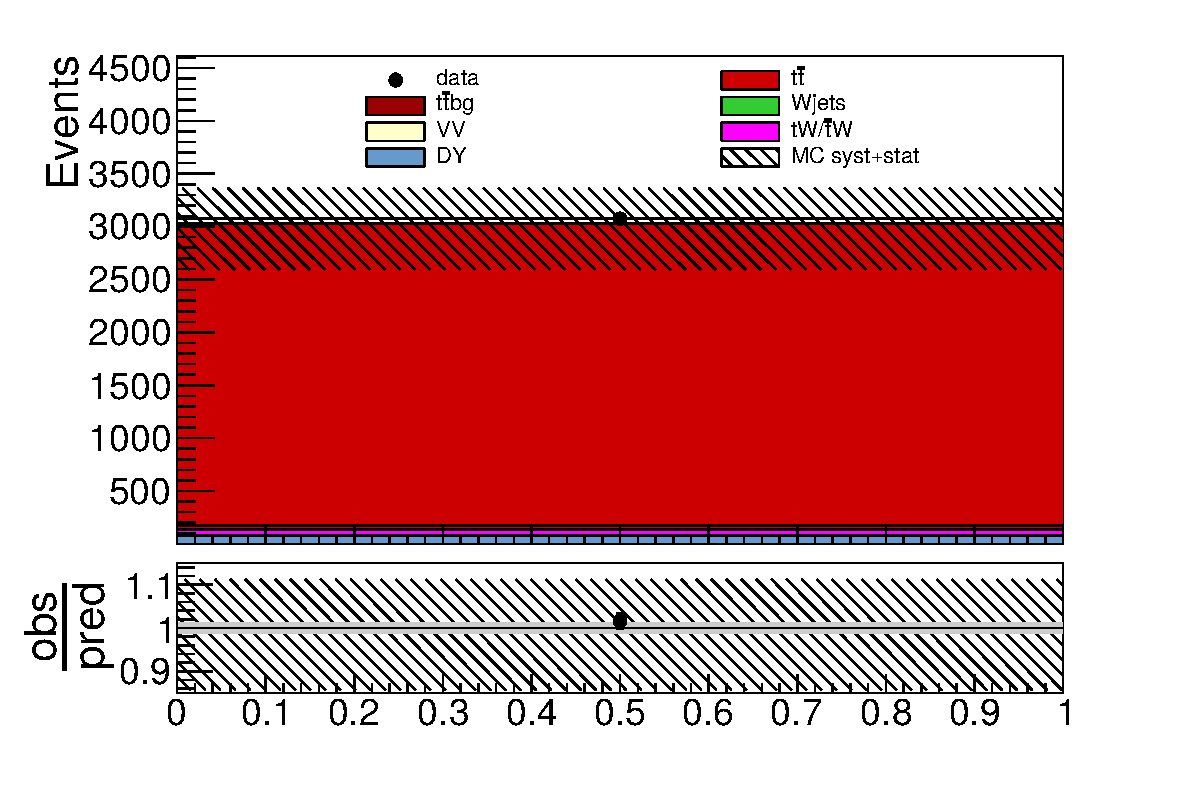
\includegraphics{CrossSection/Figures/ControlPlots/ee_sysnom/total_2_0_b-jets_step_8.pdf}}\\

    \resizebox{0.4 \textwidth}{!}{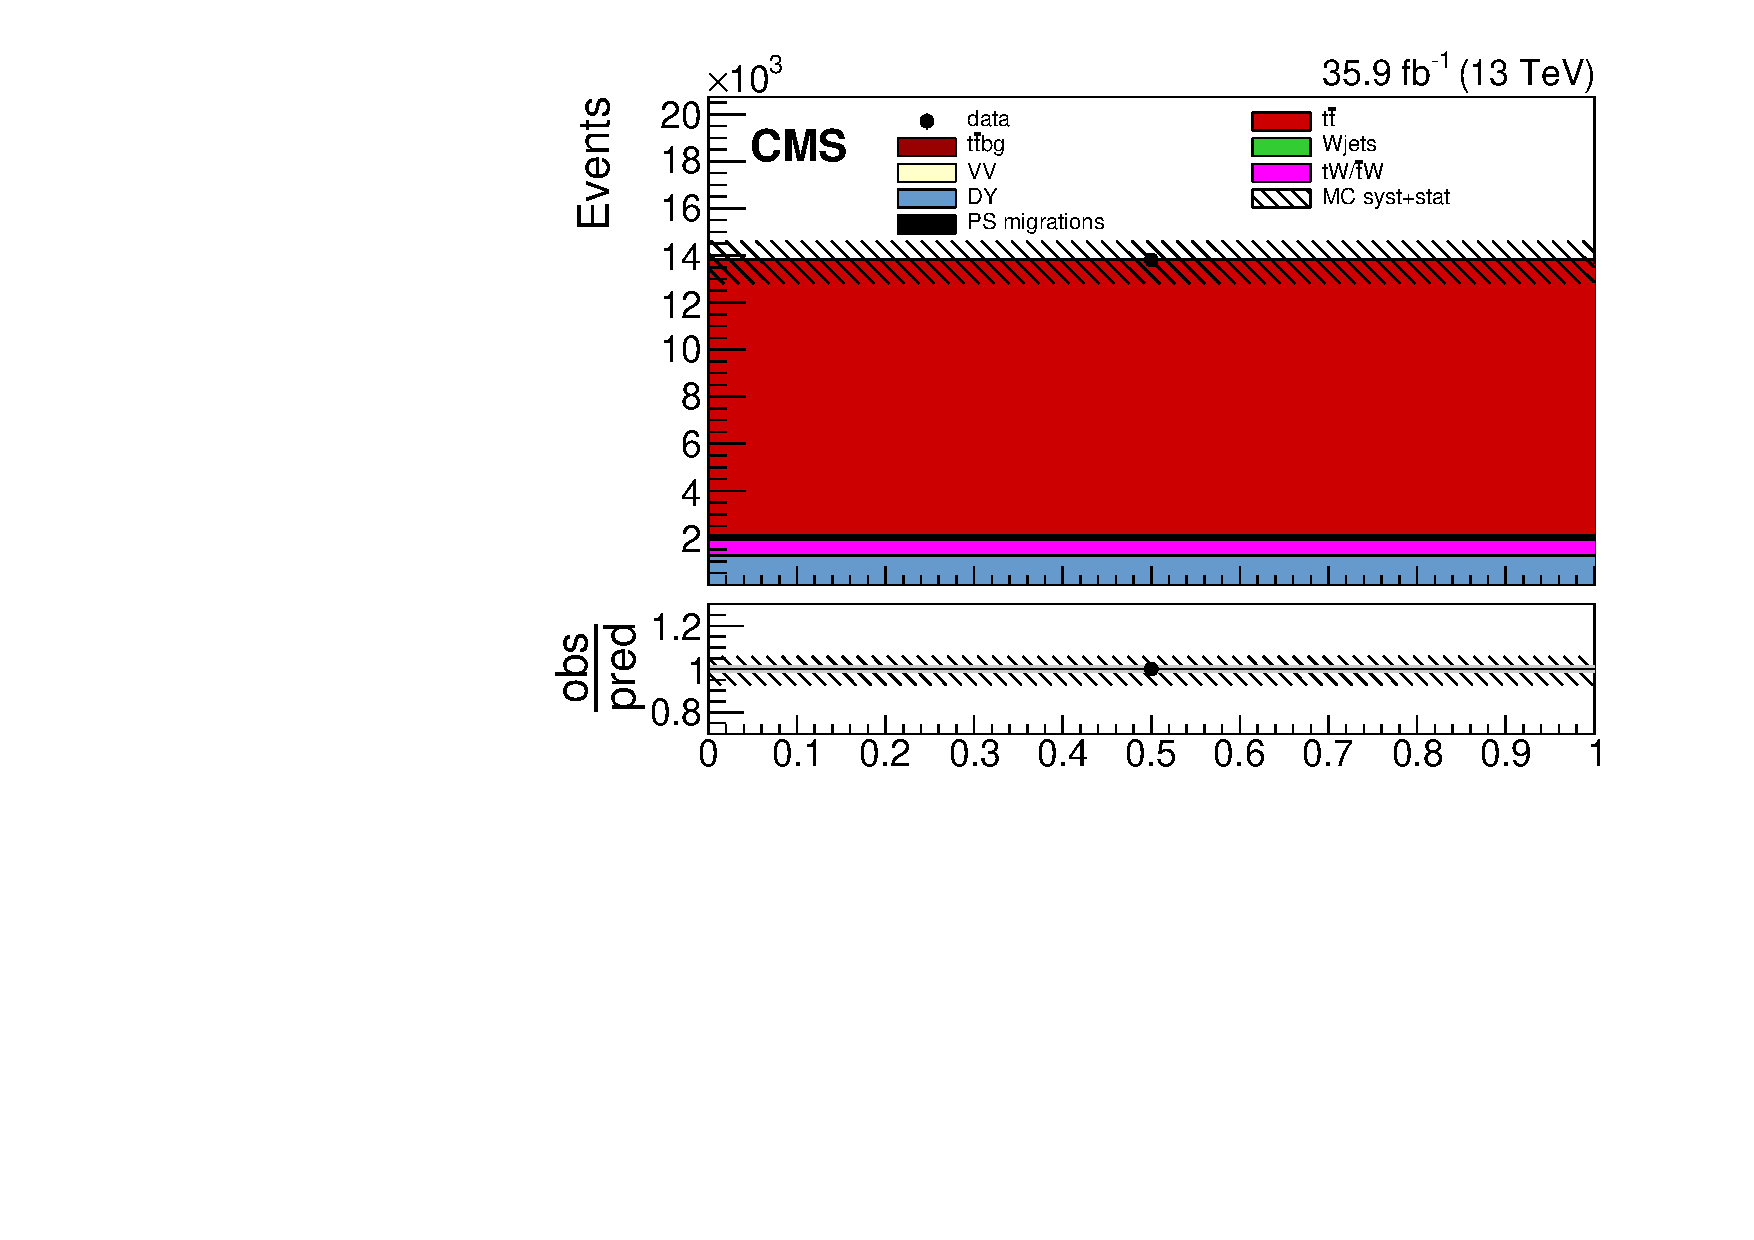
\includegraphics{CrossSection/Figures/ControlPlots/ee_sysnom/total_1_1_b-jets_step_8.pdf}}
    \resizebox{0.4 \textwidth}{!}{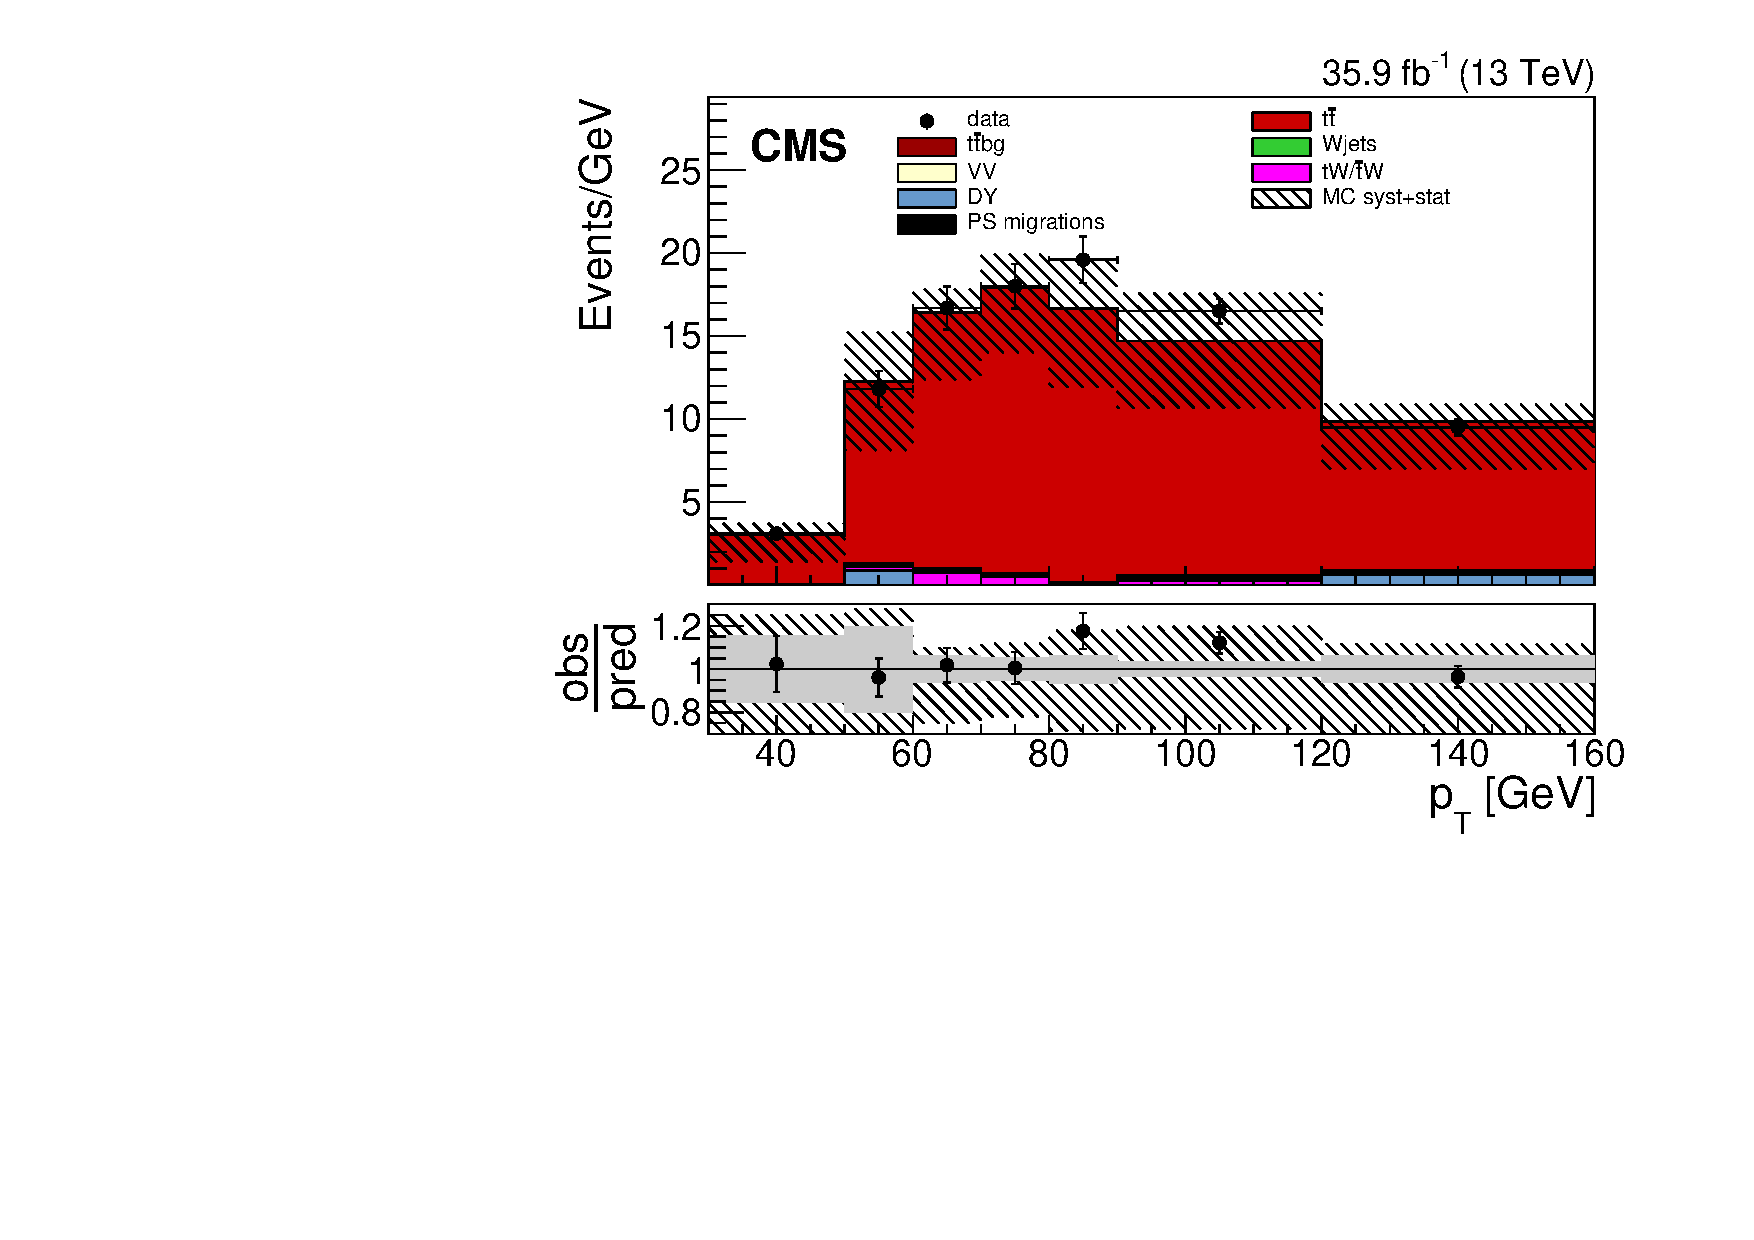
\includegraphics{CrossSection/Figures/ControlPlots/ee_sysnom/lead_jet_pt_2_1_b-jets_step_8.pdf}}\\
        
    \resizebox{0.4 \textwidth}{!}{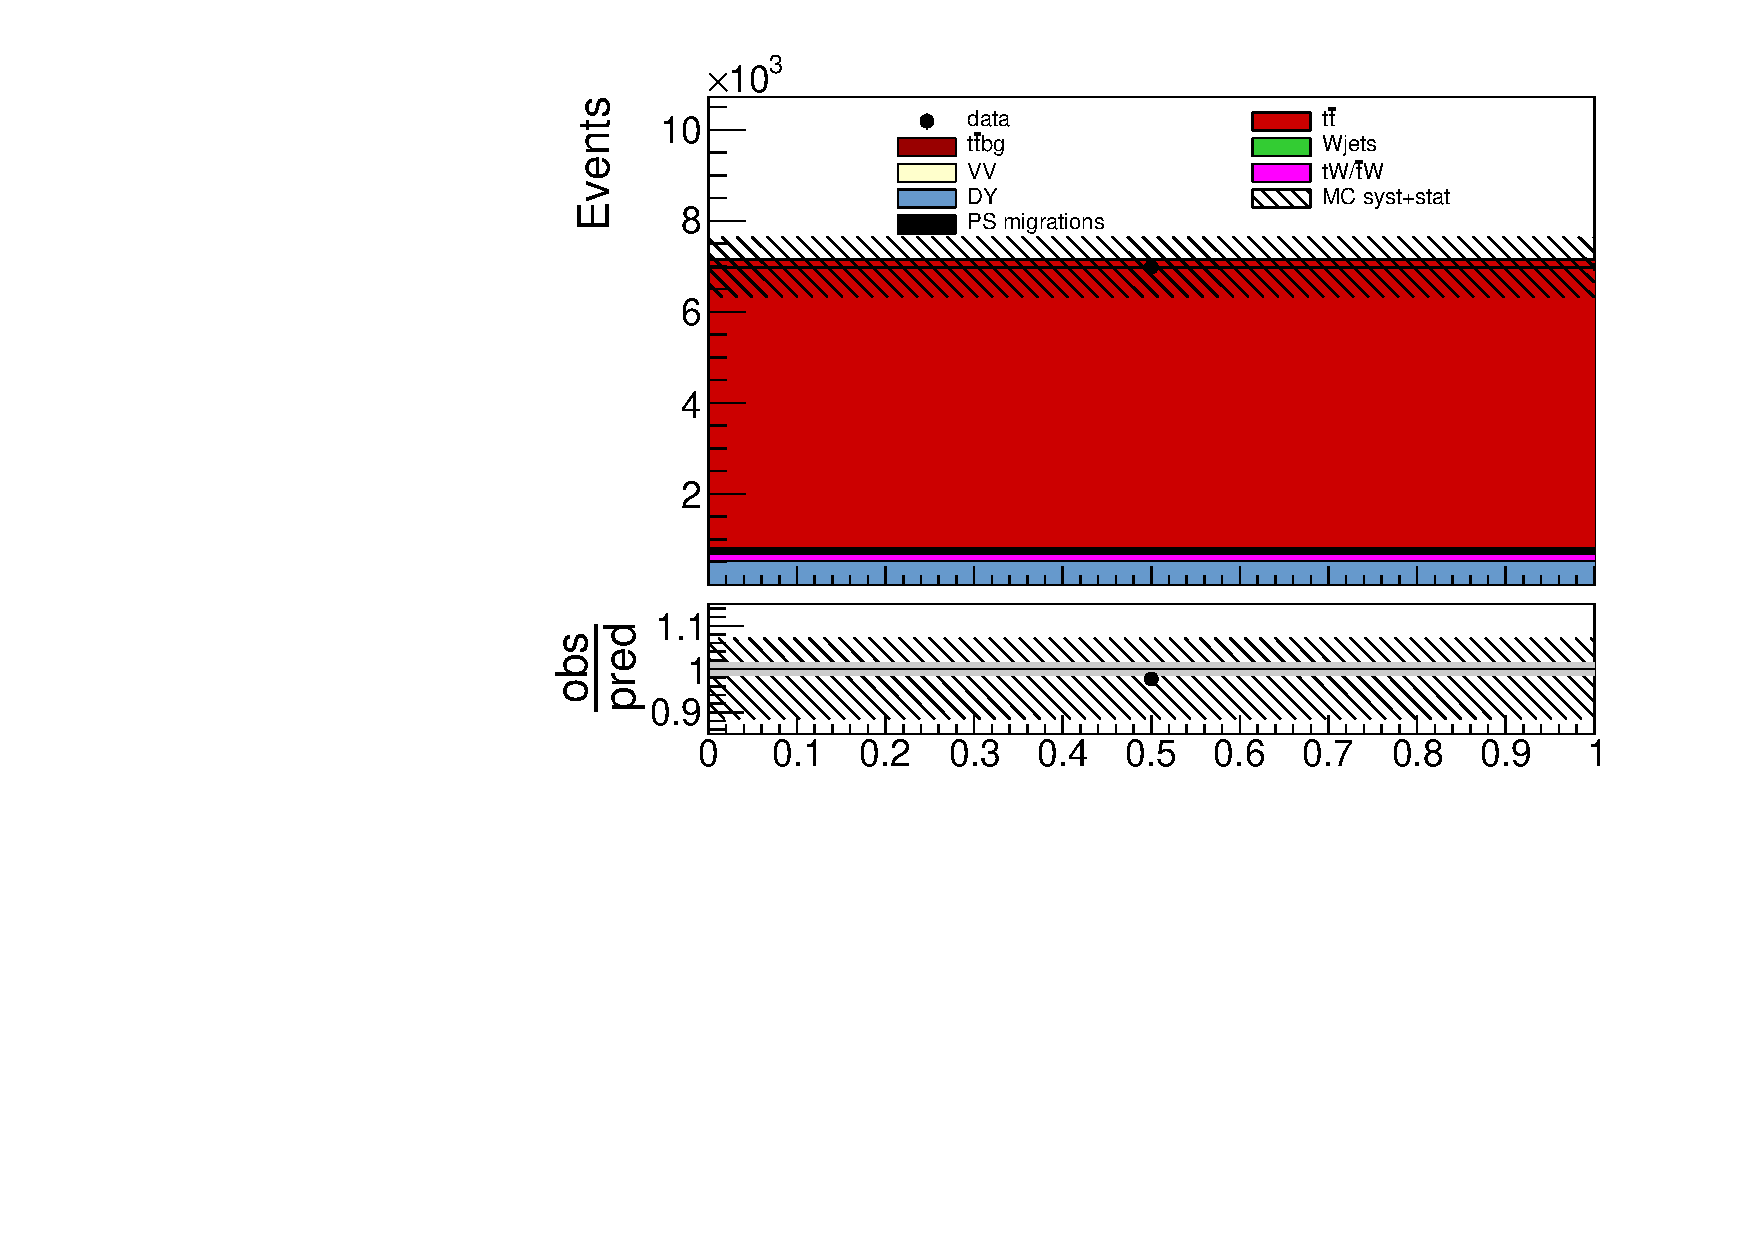
\includegraphics{CrossSection/Figures/ControlPlots/ee_sysnom/total_1_2_b-jets_step_8.pdf}}
    \resizebox{0.4 \textwidth}{!}{\includegraphics{CrossSection/Figures/ControlPlots/ee_sysnom/second_jet_pt_2_2_b-jets_step_8.pdf}}\\

    \resizebox{0.4 \textwidth}{!}{\includegraphics{CrossSection/Figures/ControlPlots/ee_sysnom/total_1_3_b-jets_step_8.pdf}}
    \resizebox{0.4 \textwidth}{!}{\includegraphics{CrossSection/Figures/ControlPlots/ee_sysnom/third_jet_pt_2_3_b-jets_step_8.pdf}} 
\caption{Pre-Fit distributions (\ee channel): 
  The left column shows events with one b-tagged jet and the total event yield for events with zero (top), one (second from top)
  two (second from bottom) or three or more additional jets (bottom).
  The right column shows events with two b-tagged jets and the total yield for events with zero additional jets (top),
  the trailing jet pt for one (second from top),
  two (second from bottom) or three or more (bottom) additional jets.
  The hatched bands correspond to the total uncertainty on the sum of
  the predicted yields. The ratios of data to the sum of the
  predicted yields are shown at the bottom of each plot. Here, the solid
  gray band represents the contribution of the statistical uncertainty.  
       \label{fig:xsec_ee_inputdistr}}
  \end{center}
\end{figure}


	
\subsection{The Fitting Procedure}
\label{sec:xsec_stat}

Following the description in Section \ref{sec:xsec_fit} a binned $\chi^2$ fit is used to extract the cross section and other free parameters.
The basic expression that is minimised can be expressed in the following way:

\begin{equation}
  \chi^2  = \sum_{i} \frac{(n_i-\mu_i)^2}{n_i + \delta_{\mu_i}^2} + \sum_{l} \pi(\omega_l) + \sum_{m} \pi(\lambda_m)
\label{eq:xsec_chisqfunct}
\end{equation}

Here the index $i$ represents a single bin, while $n_i$ is the number of measured events in data, whereas $\mu_i$ is the number
of expected events in simulation. The statistical uncertainty on the expected number of events is introduced in the term $\delta_{\mu_i}$ The terms $\omega_l$ denote the uncertainty on the normalisation of the background contribution and $\lambda_m$
denotes the penalty terms for nuisance parameters with gaussian priors. For these nuisance parameters a unit normal distribution is chosen as penalty term. Nuisance parameters with a uniform prior don't contribute to the penalty terms.
The number of expected events and its uncertainty both depend on the background normalization and all further nuisance parameters.

The events contain a signal as well as a background contribution so $\mu_i$ be written as:

\begin{equation}
\mu_i = s_i(\stt,\vec{\lambda}) 
+ \sum_{l} b_{l,i}(\omega_l,\vec{\lambda}),
\label{eq:xsec_expectev}
\end{equation} 

Here $i$ again denotes the bin, while $l$ denotes the background process. The number of signal events $s_i$ depends on the \ttbar cross section $\stt$ and the nuisance parameters $\vec{\lambda}$.
The number of background events for each background process $b_{l,i}$ also depends on the nuisance parameters and the normalisation of the respective background process $\omega_l$.
In general nuisance parameters related to the detector affect both background and signal, while uncertainties affecting the theory predictions only affect the respective background or signal prediction (see Section \todo{Link to systematics chapter}).


The number of background events as used in Equation \ref{eq:xsec_expectev} can be decomposed as :

\begin{equation}
b_{l,i} = b_{l,i}^{MC} \cdot (1 + \gamma_l \omega_l),
\label{eq:nbli}
\end{equation}

Here $b_{l,i}^{MC}$ denotes the expected number of events from the simulation of the respective background process and $\gamma_l$ denotes its uncertainty.

Following the principles given in Section \ref{sec:xsec_fit}  the number of signal events can be further devided according to the number of b-tagged jets.
Since each of the top quarks decays into a W boson and a b quark it can be assumed that every \ttbar event should contain two jets originating from a b quark.
Any decays of a top quark to a W boson and a light quark can be considered negligible.
It can therefore be assumed that selecting less than two b-tagged jets in a \ttbar event is a measure for the inefficiency of the selection of b-tagged jets.
Following this assumption the number of events in the categories for events with zero or more than two b-tagged jets $s_0$, for events with exactly one $s_1$ and for events with exactly two b-tagged jets $s_2$ can be described as shown in Equation \ref{eq:xsec_nb}. Only events in the \emu channel contribute to category $s_0$.

\begin{eqnarray}
s_0  &=& \mathcal{L}_{\rm int}\stt \epsilon_{ll} \cdot (1-2\epsilon_b(1-C_b\epsilon_b)-C_b\epsilon_b^2) \\
s_1  &=& \mathcal{L}_{\rm int} \stt \epsilon_{ll} \cdot 2 \epsilon_b(1-C_b\epsilon_b) \\
s_2  &=& \mathcal{L}_{\rm int} \stt \epsilon_{ll} \cdot   \epsilon_b^2 C_b 
\label{eq:xsec_nb}.
\end{eqnarray}

Here $\mathcal{L}_{\rm int}$ is the integrated luminosity, $\stt$ is the visible \ttbar cross section and $\epsilon_ll$ is the efficiency of the dilepton selection.
The b-tag efficiency $\epsilon_b$ includes both the efficiency of the kinematic cuts on the b-jet ($\pt > 30\; \GeV, |\eta|<2.4$) and the efficiency of the b-tagging algorithm.
It is generally assumed that the two b-jets can be identified independently of each other. Any remaining correlation is covered by the parameter $C_b$ that can also be written as
$C_b=4s_{ll}s_2/(s_1+2s_2)^2$ where $s_{ll}$ is the total number of selected events. 
The extrapolation to the full phase space using the acceptance will be described in the next section.

Within the fit, the MC simulated quantities $\epsilon_{ll}$, $b_{l,i}$ and $s_{i}$ are taken from simulation and depend on the nuisance parameters $\vec{\lambda}$.
This dependece is modeled with a second order polynomial which is constructed using the nominal and the two systematically varied values of each nuisance parameters $\lambda_m=0,1,-1$.
Some nuisance parameters are based on a one-sided variation so one systematically varied value exists. In these cases the dependence of the simulated quantities is modeled by a linear function.

The MINUIT~\cite{James:1975dr} algorithm is used to minimize the  $\chi^2$ term (see \ref{eq:xsec_chisqfunct} ) as function of the free fit parameters $\stt$, $\vec{\omega}$
and $\vec{\lambda}$. 

\todo{Describe stat model when its final}


\subsection{Extrapolation from the visible to the Full Phase Space}
\label{sec:xsec_extraction}

The previous explanation only dealt with the visible cross section in the visible phase space. In order to extrapolate that result to the full phase space the acceptance
needs to be considered.

The acceptance can be introduced by replacing the efficiency of the dilepton selection as follows:

\begin{equation}
\epsilon_{ll} = A_{ll} \epsilon^{vis}_{ll}.
\label{eq:epsacc}
\end{equation}

Here $A_{ll}$ is the acceptance and $\epsilon^{vis}_{ll}$ is the efficiency in the visible phase space, with both depending on the nuisance parameters $\vec{\lambda}$.
The acceptance is defined by the kinematic selection requirements on the leptons as given in Section \ref{sec:xsec_sel} applied on the simulation. Specifically the cuts are applied after the parton shower and before the simulation of the detector \todo{Link to simulation description}. There the two leptons are required to be part of the $t \rightarrow W b$ decay. They are further required to be within $|\eta|< 2.4$ with the 
leading lepton having $\pt > 25 \; \GeV$ and the trailing lepton $\pt > 20 \; \GeV$. The invariant mass of the dilepton system is required to be $\mll > 20 \; \GeV$.
These cuts correspond to the selection in the \emu decay channel.

Since the acceptance should only be constrained within the visible phase space, it should be unconstrained for the extrapolation.
This applies to uncertainties on the theory prediction which affect the fraction of events in the visible phase space, especially the variation
of parameters in the matrix element generation and in the parton shower.

Overall the following uncertainties need to be extrapolated: \todo{List of uncerts, with names from syst chamber}

The extrapolation of the uncertainties takes the fitted value of each relevant nuisance parameter as central value. Then the change of acceptance for the explicit $\pm 1 \sigma$ variation is considered as the $\pm 1 \sigma$ variation on the acceptance. These additional uncertainties are then added to the result from the fit in the fiducial phase space for each relevant nuisance parameter. These additional uncertainties are treated as uncorrelated and each is added in quadrature to the result in the fiducial phase space. This procedure can lead to assymetrical variations, even for originally symmetrical nuisance parameter in case the fitted value of the nuisance parameter is not the original central value.





